
\documentclass{gist}

\def\putepsf#1{\centering \parbox{14cm}{\epsfxsize = 14cm \epsfbox{#1}}}
\usepackage{graphicx}
\usepackage{array}
\usepackage{booktabs}
\usepackage{amsmath, amssymb}
\usepackage{tikz}
\usepackage{algorithmic}
\usepackage{bm}
\usepackage{float}
\usepackage{subcaption}  
\usepackage[dvipsnames]{xcolor}
\usepackage{hyperref}
\hypersetup{
  linkcolor  = black,
  citecolor  = olive,
  urlcolor   = black,
  colorlinks = true,
}

% yoon
\usepackage[ruled,vlined,linesnumbered]{algorithm2e}
\usepackage{etoolbox}
\AtBeginEnvironment{algorithm}{\setstretch{1.0}}
\usepackage[lofdepth=1]{subfig}
\usepackage[rightcaption]{sidecap}
\usepackage{multirow}
\usepackage{makecell}
\usepackage{url}
\usepackage{extpfeil}
\newcommand\etal{\textit{et~al.\ }}
\newcommand\eg{\textit{e.g.\ }}
\newcommand\ie{\textrm{i.e.\ }}
% yoon

\usepackage{theorem}
\usepackage{multirow}
\usepackage{setspace}
\usepackage{appendix}
\usepackage{url}

\newtheorem{theorem}{Theorem}[section]
\newtheorem{lemma}[theorem]{Lemma}
\newtheorem{corollary}[theorem]{Corollary}

\newenvironment{definition}[1][Definition]{\begin{trivlist}
\item[\hskip \labelsep {\bfseries #1}]}{\end{trivlist}}
\newenvironment{proof}[1][Proof]{\begin{trivlist}
\item[\hskip \labelsep {\bfseries #1}]}{\end{trivlist}}
\newenvironment{example}[1][Example]{\begin{trivlist}
\item[\hskip \labelsep {\bfseries #1}]}{\end{trivlist}}
\newenvironment{remark}[1][Remark]{\begin{trivlist}
\item[\hskip \labelsep {\bfseries #1}]}{\end{trivlist}}

\newcommand{\qed}{\nobreak \ifvmode \relax \else
      \ifdim\lastskip<1.5em \hskip-\lastskip
      \hskip1.5em plus0em minus0.5em \fi \nobreak
      \vrule height0.75em width0.5em depth0.25em\fi}

%-----------------------------------------------------------------------
% Department code list
% IC - Information and Communications
% IM - Information and Mechatronics
% EC - Electric Engineering and Computer Science
% MS - Materials Science and Engineering
% ME - Mechanical Engineering
% EN - Earth Science and Environmental Engineering
% LS - Life Science
% PH - Physics and Photon Science
% CH - Chemistry
% NA - Nanobio Materials and Electronics
% MD - Biomedical Science and Engineering
% ET - Integrated Technology 에너지 융합 학제
% CT - Integrated Technology 문화기술 융합 학제
% RT - Integrated Technology 지능로봇프로그램

% Department code
%\code{{BS/}{EC}}
\code{{MS/}{ME}} % 학위와 소속 코드, 초록 페이지에 나타남
%\code{{PhD/}{EC}}
%-----------------------------------------------------------------------
% Thesis title in English
% Insert \titlebreak where lines are to be separated.  Do not use the LaTeX command '\\'.

%\etitle{Study on Image Segmentation and Action Recognition in Computer Vision}

\etitle{Online Stator Flux Linkage Estimation of Synchronous Machines}

%\etitle{Study on Segmentation and Recognition for an Image Understanding}
%\etitle{Genetic Programming: \titlebreak New Optimization Tools for Real-World Applications}

%-----------------------------------------------------------------------
% Thesis title in Korean
% Insert \titlebreak where lines are to be separated.  Do not use the LaTeX command '\\'.
%\begin{spacing}{2.0}
\ktitle{동기전동기의 온라인 고정자 쇄교 자속 추정}
%\end{spacing}
%-----------------------------------------------------------------------
% Advisor's name in English without a position such as 'Prof.'.
\advisor{Kyunghwan Choi}

%-----------------------------------------------------------------------
% Advisor's name in Korean without a position such as 'Prof.'.
\kadvisor{최경환}

%-----------------------------------------------------------------------
% Co-advisor's name in English
% In case there is no co-advisor, comment out the following line with a "%" in the front.
%\coadvisor{My Co-advisor}

%-----------------------------------------------------------------------
% Name of the author in English
\ename{Seunghun Jang}

%-----------------------------------------------------------------------
% Name of the author in Korean seperated with '{}'.
\kname{{}{}{}{}{장}{승}{훈}} % 한글 이름 7글자까지 가능, 오른쪽 끝에 맞춰서 입력

%-----------------------------------------------------------------------
% Student ID of the author
\studentid{20221175}

%-----------------------------------------------------------------------
% The year of graduation (ex. 1999)
\coveryear{2024}

%-----------------------------------------------------------------------
% The date signed by the advisor.  The first is the month, second the date, and third the year.
\advisorsigndate{June}{12}{2024}

%-----------------------------------------------------------------------
% The date signed by the referees.  The first is the month, second the date, and third the year.
\refereesigndate{June}{12}{2024}

%-----------------------------------------------------------------------
% Names of the referees in English
% For Master's thesis, input the names of the three referees (refereeA thru referee C) in full.
% For Ph.D thesis, input the names of the five referees (refereeA thru referee E) in full.
% For most cases, refereeA is the same as the advisor.

\refereeA{Prof. Kyunghwan Choi.}
\refereeB{Prof. Pilwon Hur.}
\refereeC{Prof. Yongsoon Park.}

%-----------------------------------------------------------------------
% This is the beginning of the thesis.

%\dedication{Dedicated to my family.}

\begin{document}

%-----------------------------------------------------------------------
% Abstract of the thesis in English.
% Insert the abstract between \begin{eabstract} and \end{eabstract}.
% You can either write the abstract directly here or import a file using the \input command.

%%%%%%%%%%%%%%%%%%%%%%%%%%%%%%%%%%%%%%%%%%
% Abstract by English
%%%%%%%%%%%%%%%%%%%%%%%%%%%%%%%%%%%%%%%%%%

\begin{eabstract}
\begin{spacing}{2.0} % double spacing

%%%%%%%%%%%%%%%%%%%%%%%%%%%%%%%%%%%%%%
% Abstract of the thesis in English
%%%%%%%%%%%%%%%%%%%%%%%%%%%%%%%%%%%%%%
In this thesis, online flux linkage estimators for synchronous machines (SMs) are proposed. The proposed flux estimators are generally applicable to all types of synchronous machines and are designed to consider the nonlinearities caused by cross-coupling and magnetic saturation in the machines. Additionally, the estimators are designed without using filters designed in the frequency domain, thus avoiding phase and magnitude distortions in transient state. Existing estimators primarily determine their estimation performance in both transient and steady states based on the accuracy of the nominal parameters. However, the proposed estimators assume the nonlinear flux term as a ramp disturbance signal or estimate parameters online and update them to the actual values, thereby reducing the impact of parameter inaccuracies. This improves the flux estimation performance under various operating conditions. The validity of the proposed estimators is demonstrated through
comparisons with existing estimators with finite element method (FEM)-based simulations of a 35 kW Interior Permanent Magnet Synchronous Motor (IPMSM) provided
in MATLAB/Simulink.

\textbf{Keywords:} Synchronous machines (SMs), nonlinear flux linkage, online estimation, parameter update 

\end{spacing}
\end{eabstract}

%-----------------------------------------------------------------------
% Abstract of the thesis in Korean.
% Insert the abstract between \begin{kabstract} and \end{kabstract}.
% You can either write the abstract directly here or import a file using the \input command.

%%%%%%%%%%%%%%%%%%%%%%%%%%%%%%%%%%%%%%%%%%
% Abstract by Korean
%%%%%%%%%%%%%%%%%%%%%%%%%%%%%%%%%%%%%%%%%%

\begin{kabstract}
\begin{spacing}{2.0} % double spacing

%국문초록
%%%%%%%%%%%%%%%%%%%%%%%%%%%%%%%%%%%%%%
% Abstract of the thesis in Korean
%%%%%%%%%%%%%%%%%%%%%%%%%%%%%%%%%%%%%%
본 논문에서는 실시간으로 동기전동기(Synchronous Machines)의 비선형 쇄교 자속을 추정할 수 있는 추정기들을 제안한다. 제안된 자속 추정기들은 모든 동기기에 일반적으로 적용 가능하며, 동기기의 교차 결합 및 자기 포화로 인한 비선형성을 고려하여 설계되었다. 또한, 주파수 영역에서 설계된 필터를 사용하지 않고 추정기를 설계하여 과도 상태에서의 추정치에 위상 및 크기 왜곡이 발생하지 않는다. 기존의 추정기들은 공칭 파라미터의 정확성에 따라 과도 및 정상 상태에서의 추정 성능이 결정된다. 그러나 제안된 추정기들은 비선형 자속 항을 일정한 기울기를 가진 외란 신호로 가정하거나, 실시간으로 파라미터를 추정하여 실제 값으로 업데이트함으로써 파라미터 부정확성으로 인한 영향을 줄일 수 있으므로 이를 통해 다양한 운전 조건에서 자속 추정 성능을 향상시킨다. 제안된 추정기들은 매트랩/시뮬링크에서 제공하는 유한 요소법 기반의 35 kW IPMSM 시뮬레이션을 통해 기존의 추정 방식들과 비교 및 검증하여 그 타당성을 입증하였다.

\textbf{주요어:} 동기전동기, 비선형 쇄교자속, 실시간 추정, 파라미터 업데이트 


\end{spacing}
\end{kabstract}


%-----------------------------------------------------------------------
% Table of contents, list of tables and list of figures.
% Use the \makecontents command to automatically generate the table of content
\makecontents

% In case there is no table, comment out the following line.
\listtables

% In case there is no figure, comment out the following line.
\listfigures

% In case there is no algorithm, comment out the following line.
\listalgorithms
%-----------------------------------------------------------------------
% Input the thesis files written in LaTeX.
% The \begin{document} command is not necessary here.
% Refererence and vitae will folllow the main thesis text.
%-----------------------------------------------------------------------
% This is the beginning of the main thesis body.
% Insert Chapter or section or subsection as many as you need.

%%%%%%%%%%%%%%%%%%%%%
% Chapter 1 Introduction
%%%%%%%%%%%%%%%%%%%%%

%%%%%%%%%%%%%%%%%%%%%%%%%%%%%%%%%%%%%%
% DO NOT DELETE FOLLOWING TWO LINES! %
%%%%%%%%%%%%%%%%%%%%%%%%%%%%%%%%%%%%%%
\begin{spacing}{2.0} % double spacing
\pagenumbering{arabic}
\setcounter{page}{1}

% you start with the chapter 1


%%%%%%%%%%%%%%%%%%%%%%%%%%%%%%%%
% Chap 1. Introduction
%%%%%%%%%%%%%%%%%%%%%%%%%%%%%%%%

\chapter{Introduction}\label{chapter1}
\section{Motivation} \label{chap1:sec1}

Synchronous machines (SMs) have advantages such as high drive efficiency, output torque, power density, and excellent control performance \cite{c1_5},\cite{c2.1_1}. These advantages have led to their extensive use in various industries, including high-performance control applications such as servo systems \cite{c1_3} and home appliances \cite{c1_6}, as well as in renewable energy and eco-friendly sectors like wind power generators \cite{c1_4} and hybrid and electric vehicles \cite{c1_7},\cite{c1_8}.

Synchronous machines (SMs) are generally classified into three types: Permanent Magnet Synchronous Motor (PMSM), which has the same or different $d$-$q$ axis stator inductances and a rotor with embedded permanent magnets; Synchronous Reluctance Motor (synRM), which has different $d$-$q$ axis inductances due to the anisotropic rotor design that lacks permanent magnets and relies on rotor saliency for torque production; and Permanent Magnet-Assisted Synchronous Reluctance Motor (PMa-SynRM), which combines permanent magnets with a reluctance rotor to enhance torque production and efficiency. By appropriately utilizing the permanent magnets and the additional reluctance torque of these SMs, it is possible to maintain high output torque and efficiency over a wide operating range from low to high mechanical speeds. Therefore, due to these advantages, many automotive manufacturers have adopted SMs as traction motors for electric vehicles \cite{c1_7} (as shown in Table \ref{Table:1.1}).

\begin{table}[t]
\centering
\begin{tabular}{c|c|c|c|c|c}
\toprule
\hline
 & BMW i3 (2016) & Leaf2012 & Bosch SMG & Prius & McLaren\\
\hline
Motor type & IPM & IPM & PM & PM & SPM\\
\hline
Power density (kW/L) & 9.1 & 4.2 & 9.5 & 4.8 & -\\
\hline
Specific power (kW/kg) & 3.0 & 1.4 & 2.5 & 1.6 & 4.6\\
\hline
Max torque (Nm) & 250 & 207 & 198 & 207 & 130 \\
\hline
Max power (kW) & 125 & 80 & 80 & 60 & 120 \\
\hline
Max efficiency ($\%$) & 94 & 97 & 97 & 96 & 96 \\ 
\hline
\bottomrule
\end{tabular}
\caption{Specifications of EV traction motors in \cite{c1_7}.}
\label{Table:1.1}
\end{table}

In general, SMs generate torque through the interaction of the rotating magnetic fields produced by the stator and rotor, making stator flux linkage information crucial for controlling the torque of SMs. However, since flux cannot be directly measured by sensors, it is indirectly expressed using the machine parameters of the SMs (inductance, permanent magnet flux linkage) and the measurable stator current, allowing the SMs torque to be represented using these parameters and the current. 

These machine parameters of SMs are commonly used in fault diagnosis algorithms for detecting stator winding short circuits and demagnetization. These algorithms can enhance the reliability and efficiency of SMs by continuously monitoring them and predicting necessary maintenance tasks \cite{c1_9},\cite{c1_10},\cite{c1_11},\cite{c1_12},\cite{c1_13}. In addition, these parameters are also used in various optimal torque control strategies to minimize copper losses caused by the current in the stator windings, thereby increasing output efficiency and torque \cite{c1_2},\cite{c1_14}. In general, there are limitations to directly controlling the desired torque reference of SMs; it is necessary to convert the torque command into current references. However, since the output torque can be expressed as a bilinear function of the d- and q-axis currents, there are infinite combinations of d- and q-axis stator currents that can produce the same torque. Thus, these current combinations can be typically determined using the maximum torque per ampere (MTPA) control method, which maximizes torque per unit of current. However, when the mechanical speed of the synchronous machine exceeds the base speed, the increased back electromotive force (EMF) results in a limitation of the input voltage, making it impossible to maintain MTPA operation. Therefore, field weakening control is applied, which involves controlling the $d$-axis current to negative values to suppress the influence of the back EMF. Therefore, to optimally control the torque of the SMs and accurately implement these approaches, precise parameter information is ultimately essential. Moreover, the current references generated by the current reference generator can be optimally controlled through feedforward compensation-based current control or advanced optimal control based on model predictive control strategies \cite{c1_15},\cite{c1_16} such as Continuous Control Set Model Predictive Control (CCS-MPC) or Finite Control Set Model Predictive Control (FCS-MPC), for which accurate parameter or flux linkage information is necessary.

However, these parameters vary with the operating conditions of SMs, which are affected by the temperature of the stator windings, currents, and the temperature of the permanent magnets \cite{c1_17},\cite{c1_18}. To address these issues, several studies have presented adaptive-based methods for online estimation of multiple parameters \cite{c1_19},\cite{c1_20}, but these approaches fail to ensure estimation convergence. Some studies have suggested high-frequency current signal injection methods \cite{c2.3_3},\cite{c1_21} to temporarily resolve the rank deficiency issue and estimate parameters. Nevertheless, these approaches cause additional core losses reducing the efficiency of the synchronous machine, and fail to consider the inductance variation with $d$-$q$ axis current resulting in decreased accuracy of inductance estimation at the flux saturation region \cite{c1_22}. As a result of the absence of an accurate solution for online parameter estimation, the industry conventionally relies on 2-dimension lookup tables (LUTs) that list parameter information obtained through extensive experiments at all operating conditions \cite{c1_23},\cite{c1_25}. However using LUTs has several drawbacks because these tables require significant time and costly experimental resources, and interpolation must be used, which can degrade control performance due to errors with the actual parameters when operating the synchronous machine. Additionally, since LUTs are typically based on parameter information from a single motor sample, it is difficult to apply them uniformly to all synchronous machines due to parameter variations caused by manufacturing tolerances, aging, or temperature changes \cite{c1_24}.

In this background, a method for estimating parameters online without relying on LUTs is necessary to successfully operate SMs. As mentioned above, it is challenging to directly estimate the inductance and permanent magnet flux linkage parameters due to the rank deficiency of the estimation model. Instead of directly estimating these parameters, the stator flux linkage can be used, as it can be expressed as either the static inductance \cite{c2.1_3}, which has a linear relationship with the stator current, or the dynamic inductance \cite{c2.1_3},\cite{c1_26}, which has a nonlinear relationship with the stator current considering the magnetic saturation and cross-coupling effects. Thus, if the accurate stator flux linkage can be estimated online, it becomes possible to estimate these inductances online, making it necessary to first develop a high-performance stator flux linkage estimator.

\section{Research Objectives} \label{chap1:sec2}

Since the machine parameters of SMs continuously vary due to changes in temperature, speed, and current, a flux linkage estimator capable of online estimation of flux linkage or parameters is necessary to enhance the reliability and control performance of SMs. However, the estimation performance of existing flux estimators (especially transient estimation performance) is determined by the filters or nominal parameters used in the estimators. 

Therefore, the objectives of this study are (i) to develop an observable estimation model based on the stator flux linkage dynamics, (ii) to design a state observer in the time domain without relying on filters to improve estimation performance, and (iii) to develop a flux estimator that reduces dependence on nominal parameters to enhance estimation performance during transient states.

\section{Outline of the Thesis} \label{chap1:sec3}
This thesis is organized as follows: In Chapter \ref{chapter1}, the background and objectives of this study are discussed. In Chapter \ref{chapter2}, the mathematical modeling of synchronous machines (with interior permanent magnet synchronous machines as an exemplary model), optimal current control based on finite control set model predictive control, and existing research on flux linkage estimation are covered. In Chapter \ref{chapter3}, two flux estimators are proposed that can address the limitations of existing estimators by reducing parameter dependency and improving transient estimation performance. In Chapter \ref{chapter4}, the proposed flux estimators are validated through simulations and compared with the existing method. Finally, the conclusion of this study and future research are discussed in Chapter \ref{chapter5}, concluding the thesis.

\end{spacing}

%%%%%%%%%%%%%%%%%%%%%%%%%%%%%%%%%%%%
% Chapter 2 
%%%%%%%%%%%%%%%%%%%%%%%%%%%%%%%%%%%%

\begin{spacing}{2.0}

%%%%%%%%%%%%%%%%%%%%%%%%%%%%%%%%
% Chap 2. Related works of action recognition
%%%%%%%%%%%%%%%%%%%%%%%%%%%%%%%%

\chapter{Preliminaries}\label{chapter2}
%1차 수정 완료
Synchronous Machines (SMs) generate electrical torque through the continuous interaction of the two rotating magnetic fields, which are generated by the stator and the rotor, so it is important to analyze the physical behavior of the stator flux linkage. In Section \ref{chap2:2.1}, the basic physical characteristics and mathematical model of SM are briefly reviewed. In general, stator flux linkage can be expressed as a nonlinear function of stator current and machine parameters, so the voltage equation of SM can be represented by the dynamics of the stator current. Therefore, current control methods for SM based on stator current dynamics are briefly introduced in Section \ref{chap2:2.2}. To properly perform these methods, accurate parameter information, such as inductances and permanent magnet flux linkages, is required. However, these parameters vary nonlinearly with the stator current and the temperature of the stator windings and rotor, affecting the control performance of the SM. Thus, Section \ref{chap2:2.3} introduces conventional approaches for online stator flux linkage estimation, which is the first step in obtaining the parameters required for current control or optimal torque control.

\section{Mathematical Model of SM}\label{chap2:2.1}
\subsubsection{Modeling in the ($a$,$b$,$c$)-reference frame}
In SM, each stator winding in the ($a$,$b$,$c$)-reference frame is connected in a Y-connection structure, and according to Kirchhoff's law, the sum of all instantaneous stator currents is zero, i.e. 
\begin{equation}\label{eqn:2.1}
i^a_s(t)+i^b_s(t)+i^c_s(t)=0, \quad \forall t \geq 0    
\end{equation}
where the voltage applied to the three-phase stator windings of an SM consists of the voltage drop across the winding resistance and the induced voltage due to the time derivative of the stator flux linkage, as described by Faraday’s law. Therefore, the mathematical model of the SM can be expressed as
\begin{equation}\label{eqn:2.2}
\mathbf{u}^{abc}_s(t) = R_s \mathbf{i}^{abc}_s(t) + \frac{d}{dt}\underbrace{\bm{\psi}^{abc}_s \left( \mathbf{i}^{abc}_s(t),\theta_r(t)\right)}_{=:\bm{\psi}^{abc}_s(t)},
\end{equation}
\begin{equation}\notag
\left(
    \theta_r(t) := n_p(\theta_m(t) + \theta_{pm})=n_p\left( \int_0^t \omega_m(\tau)d\tau + \theta_{pm}\right)
    \right)
\end{equation}
\begin{figure}[t]
    \centering
    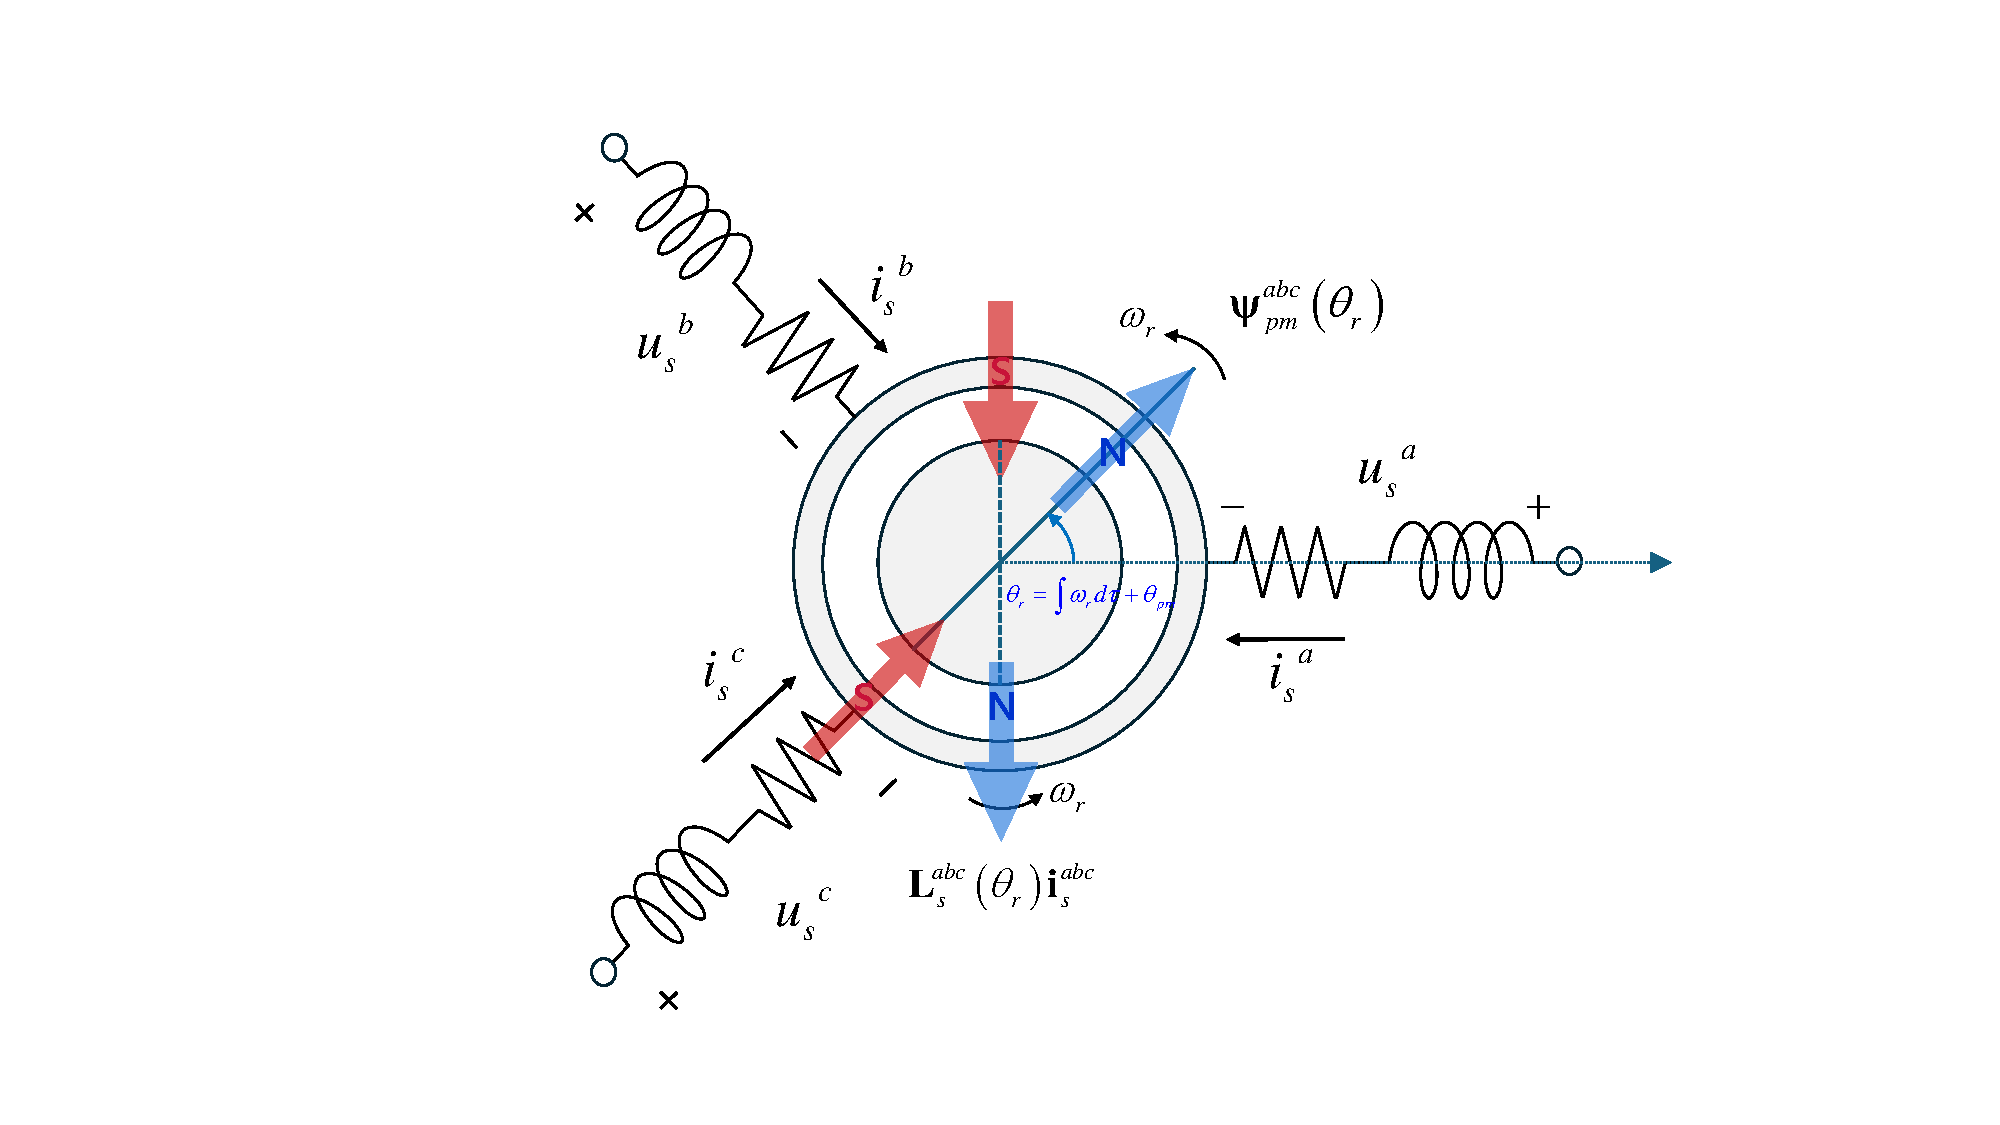
\includegraphics[scale=0.52]{chapters/Fig2.1.pdf}
    \caption{SM structure.}
    \label{Fig:2.1}
\end{figure}
where $R_s$ is the stator resistance, $\mathbf{u}^{abc}_{s} := (u^a_s, u^b_s, u^c_s)^\top$ $(\text{in } \mathbf{V} \cdot \mathbb{R}^3)$ and $\mathbf{i}^{abc}_s := (i^a_s, i^b_s, i^c_s)^\top$ $(\text{in } \mathbf{A} \cdot \mathbb{R}^3)$ denote the \emph{stator phase voltages} and \emph{stator phase currents} in the phase windings, respectively.  The linear combination of the magnetic fields produced by the phase currents and the permanent magnets in the rotor (if present) yields the \emph{overall stator flux linkages} $\boldsymbol{\psi}^{abc}_s:= (\psi^a_s, \psi^b_s, \psi^c_s)^\top$ $(\text{in } \mathbf{Wb} \cdot \mathbb{R}^3)$. $\theta_r$ and $\theta_m$ $(\text{in rad})$ denote the electrical and mechanical rotor position between the $d$-axis and the $as$-axis, which changes over time and $\theta_{pm}$ (in rad) is an orientation offset (constant) of the permanent magnets concerning the axis of phase $a$ (see Fig.\ref{Fig:2.1}). $\omega_m$ (in rad/s) is the mechanical angular velocity and  $n_p$ $(\in \mathbb{N})$ denotes the pole pair number.

As an exemplary model of a synchronous machine, the stator flux linkage vector of a synchronous machine with embedded permanent magnets in the rotor (interior permanent magnet synchronous machine, $\textbf{IPMSM}$) is given by (see Chap.5 in \cite{c2.1_1})
\begin{align}\notag
\boldsymbol{\psi}^{abc}_s\left( \mathbf{i}^{abc}_s,\theta_r\right) &= \underbrace{\begin{bmatrix}
    L^{aa}_s & L^{ab}_s & L^{ac}_s \\
    L^{ba}_s & L^{bb}_s & L^{bc}_s\\
    L^{ca}_s & L^{cb}_s & L^{cc}_s
\end{bmatrix}}_{=:\mathbf{L}^{abc}_s(\theta_r) \in \mathbb{R}^{3\times3}}\mathbf{i}^{abc}_{s} + \underbrace{\psi_{pm}\begin{bmatrix}
\cos \theta_r \\ \cos \left( \theta_r - \frac{2\pi}{3} \right) 
\\
\cos \left( \theta_r + \frac{2\pi}{3} \right)
\end{bmatrix}}_{=:\boldsymbol{\psi}^{abc}_{pm}(\theta_r)\in \mathbb{R}^{3}}\\\label{eqn:2.3}
&= \mathbf{L}^{abc}_s(\theta_r)\mathbf{i}^{abc}_{s}+\boldsymbol{\psi}^{abc}_{pm}(\theta_r),
\end{align}
in the ($a$,$b$,$c$)-reference frame with the stator inductance matrix
\begin{equation}\notag
\small
 \mathbf{L}^{abc}_s(\theta_r) := \begin{bmatrix}
L_{ls} + L_A - L_B \cos 2\theta_r & -\frac{1}{2} L_A + L_B \cos 2 \left( \theta_r - \frac{\pi}{3} \right) & -\frac{1}{2} L_A + L_B \cos 2 \left( \theta_r + \frac{\pi}{3} \right) \\
-\frac{1}{2} L_A + L_B \cos 2 \left( \theta_r - \frac{\pi}{3} \right) & L_{ls} + L_A - L_B \cos 2 \left( \theta_r + \frac{\pi}{3} \right) & -\frac{1}{2} L_A + L_B \cos 2\theta_r \\
-\frac{1}{2} L_A + L_B \cos 2 \left( \theta_r + \frac{\pi}{3} \right) & -\frac{1}{2} L_A + L_B \cos 2\theta_r & L_{ls} + L_A - L_B \cos 2 \left( \theta_r - \frac{\pi}{3} \right)
\end{bmatrix},    
\end{equation}
where $\mathbf{L}^{abc}_s$ (in $\mathbf{H=Vs/A} \cdot \mathbb{R}^{3\times3}$) is a position-dependent stator inductance matrix in the ($a$,$b$,$c$)-reference frame, where the diagonal elements denote the self-inductance, and the off-diagonal elements represent the mutual inductance. $\boldsymbol{\psi}^{abc}_{pm}$ (in $\mathbf{Wb} \cdot \mathbb{R}^{3}$) is a position-dependent \emph{permanent-magnet flux linkage vector} with a magnitude of $\psi_{pm}$. \(L_{ls}\) is the leakage inductance of the stator windings, \(L_A\) is the inductance independent of the rotor's position, and \(L_B\) is the maximum inductance that varies with rotation due to the salient rotor structure. The structure of SM and an example of the phase $as$ winding stator inductance in IPMSM are illustrated in Fig.\ref{Fig:2.1} and Fig.\ref{Fig:2.2}, respectively. 

According to equation (\ref{eqn:2.1}), if all physical signals of the three-phase winding are balanced, one physical quantity can be expressed in terms of the other two ($i^a_s(t)=-i^b_s(t)-i^c_s(t), \forall t \geq 0$). Consequently, using reference frame transformations with matrix equations, the physical quantities in the ($a$,$b$,$c$)-reference frame can be projected into either the stationary ($\alpha$,$\beta$)-reference frame or the synchronously rotating ($d$,$q$)-reference frame, which can simplify three physical quantities into two. Figure \ref{Fig:2.3} shows the reference frame transformation according to each frame.
\begin{figure}[t]
    \centering
    \begin{subfigure}[b]{0.45\textwidth}
        \centering
        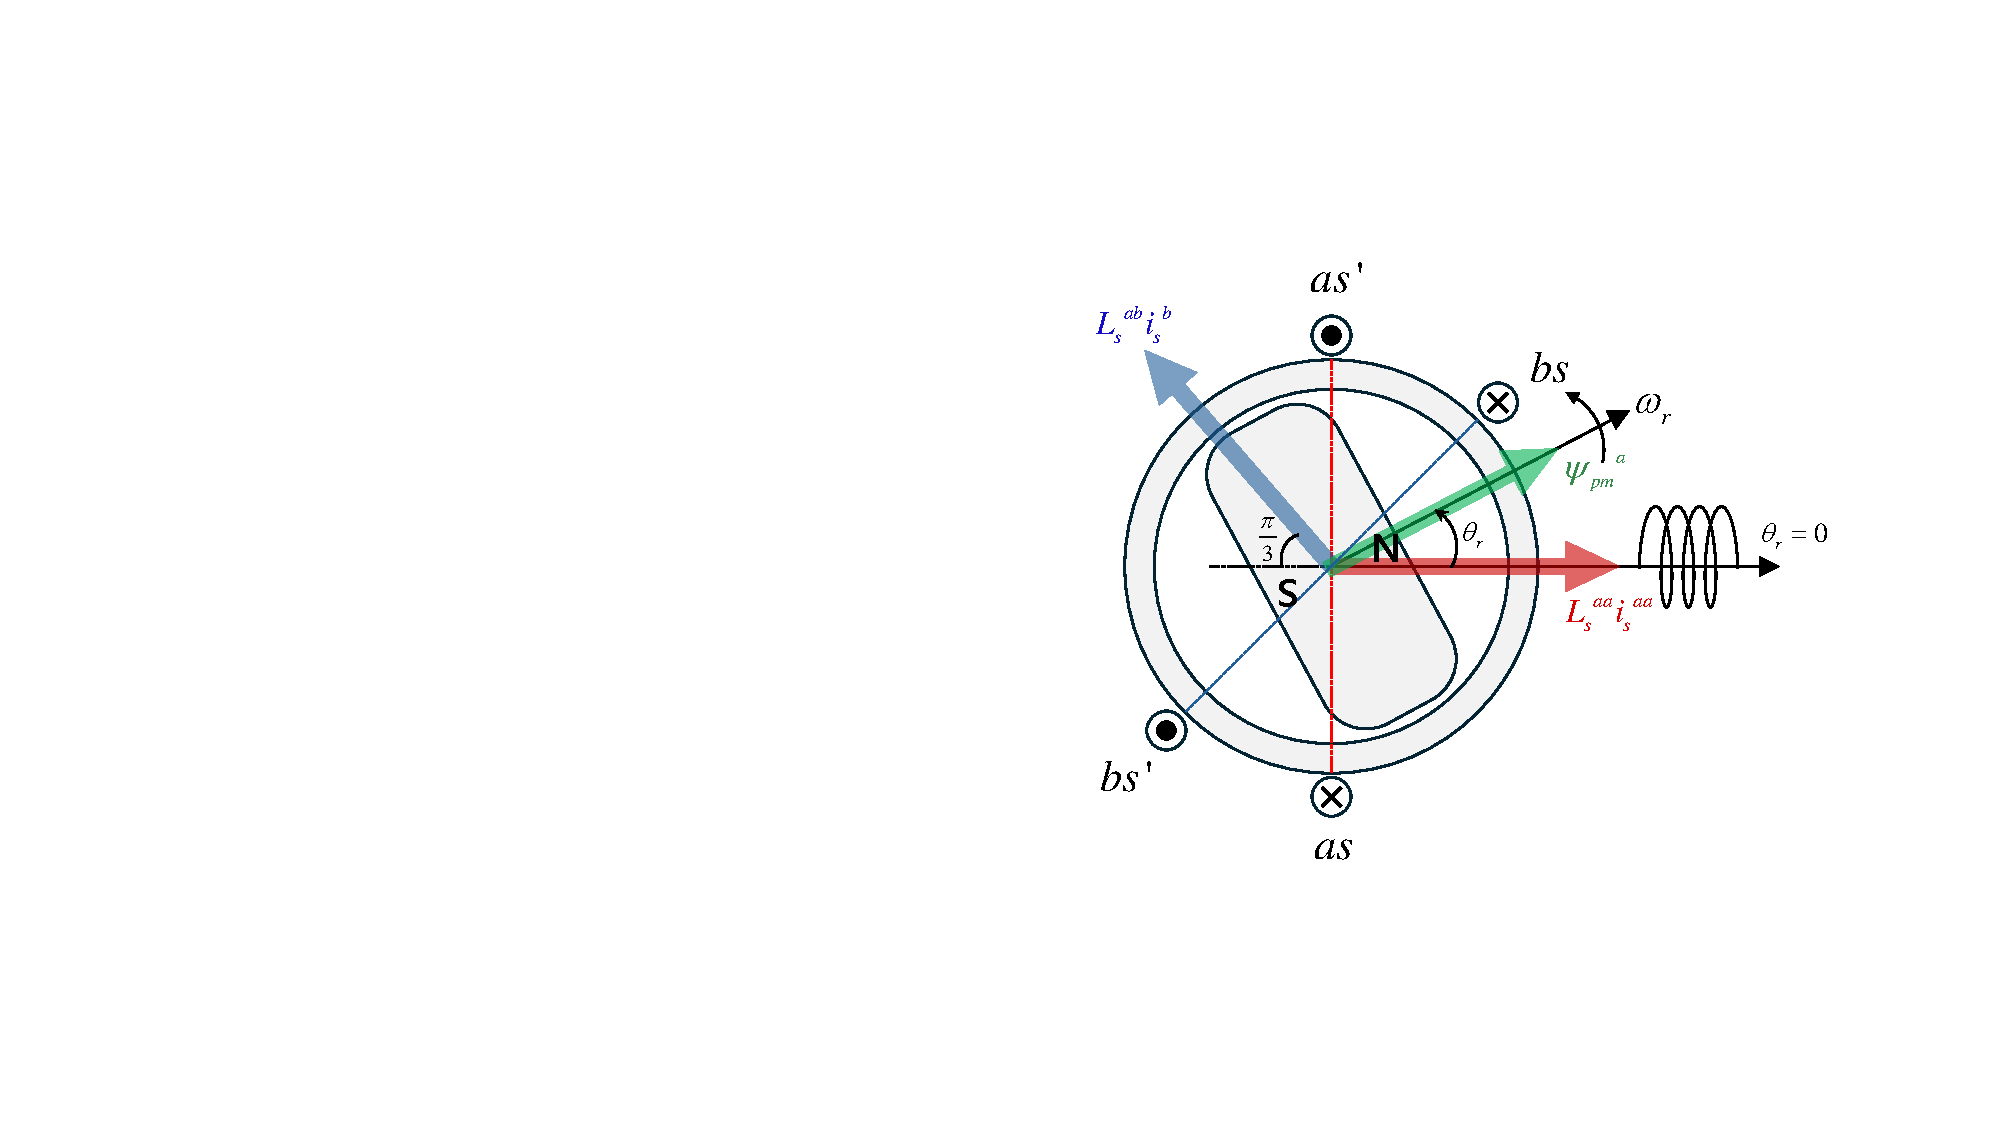
\includegraphics[scale=0.6]{chapters/Fig2.2a.pdf}
        \caption{}
        \label{Fig:2.2a}
    \end{subfigure}
    \hfill
    \begin{subfigure}[b]{0.45\textwidth}
        \centering
        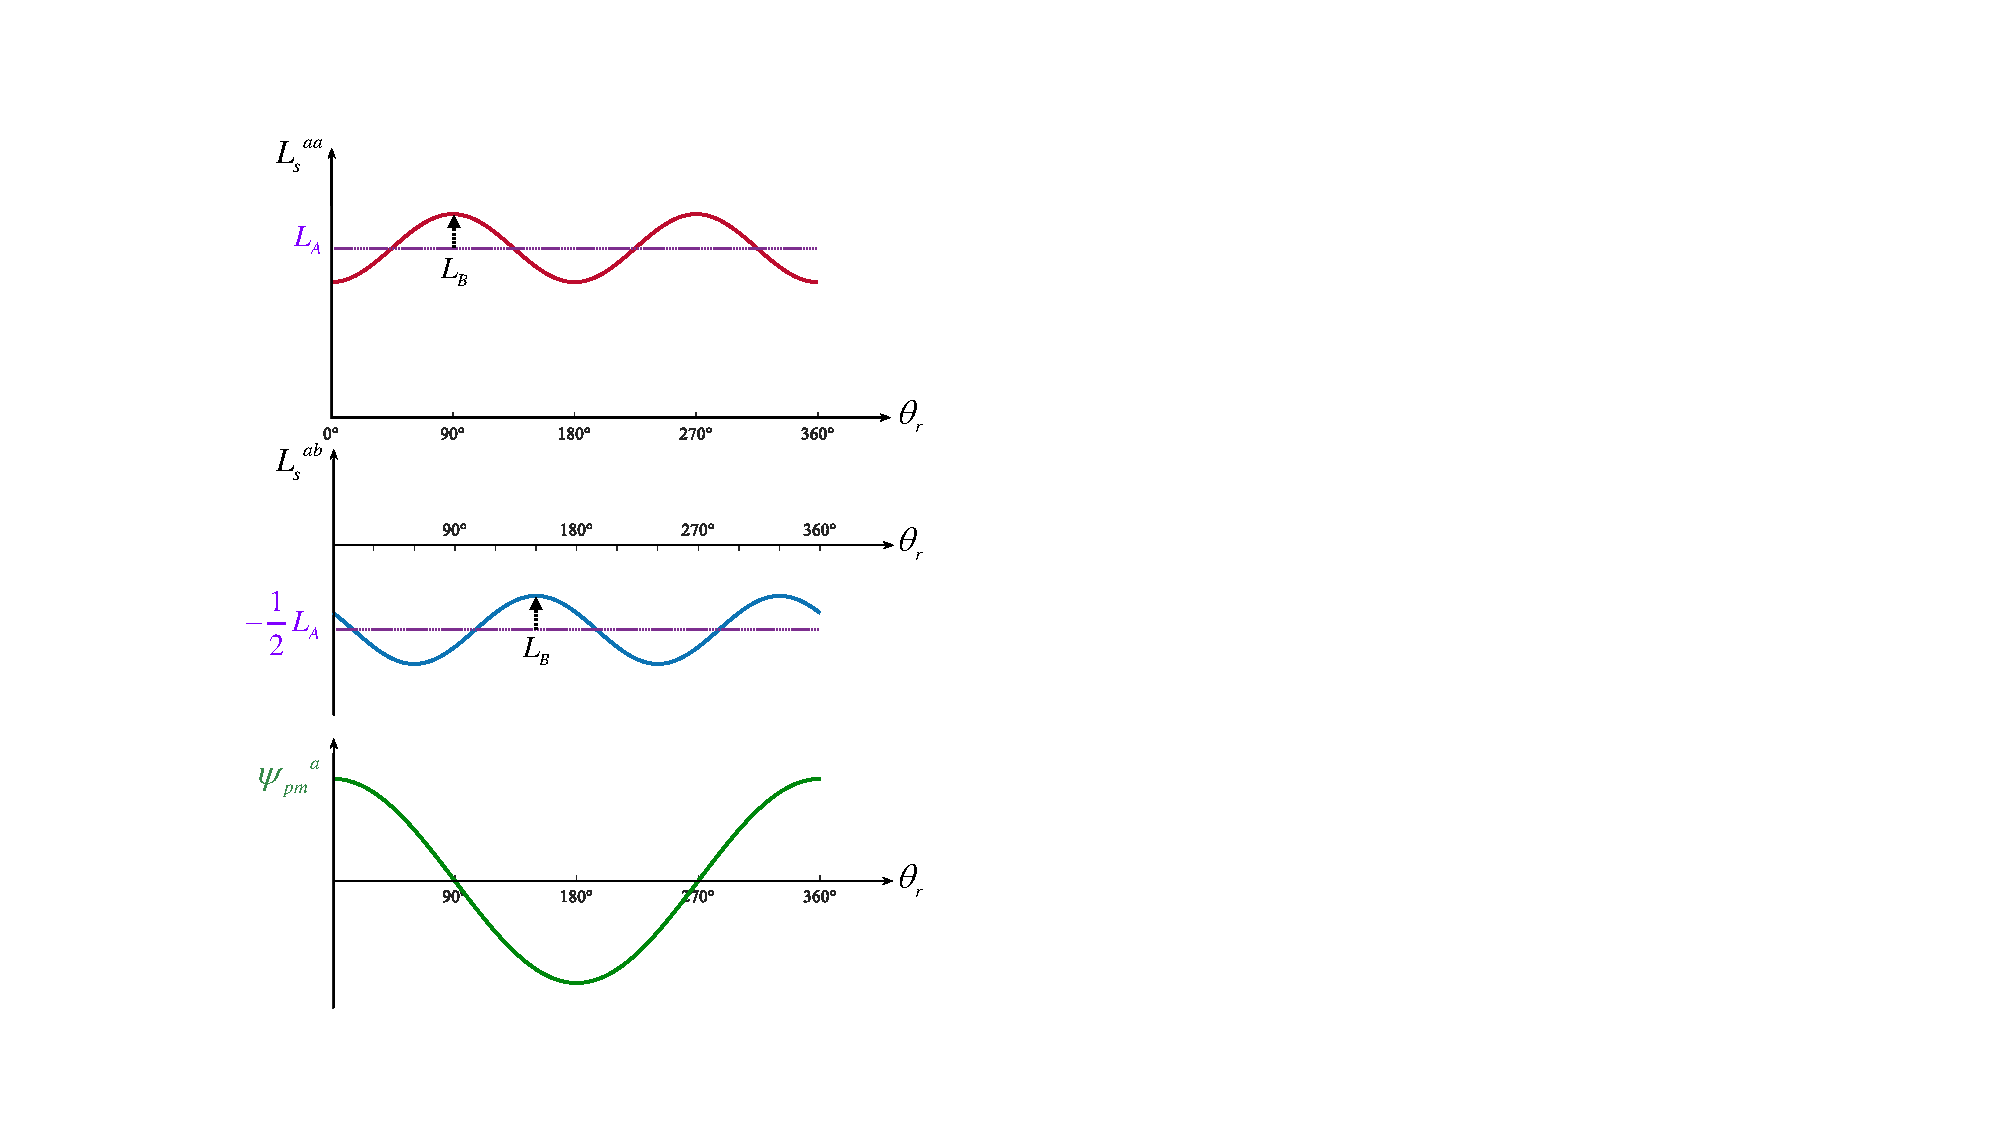
\includegraphics[scale=0.6]{chapters/Fig2.2b.pdf}
        \caption{}
        \label{Fig:2.2b}
    \end{subfigure}
    \caption{The stator inductance of phase $as$ winding for rotor positions. (a) magnetic equivalent rotor and flux linkages of an IPMSM. (b) in order, the self-inductance of the stator $as$ winding, the mutual inductance between $as$ and $bs$ phases, and the inductance between the stator $as$ winding and the magnet.}
    \label{Fig:2.2}
\end{figure}
\begin{figure}[t]
    \centering
    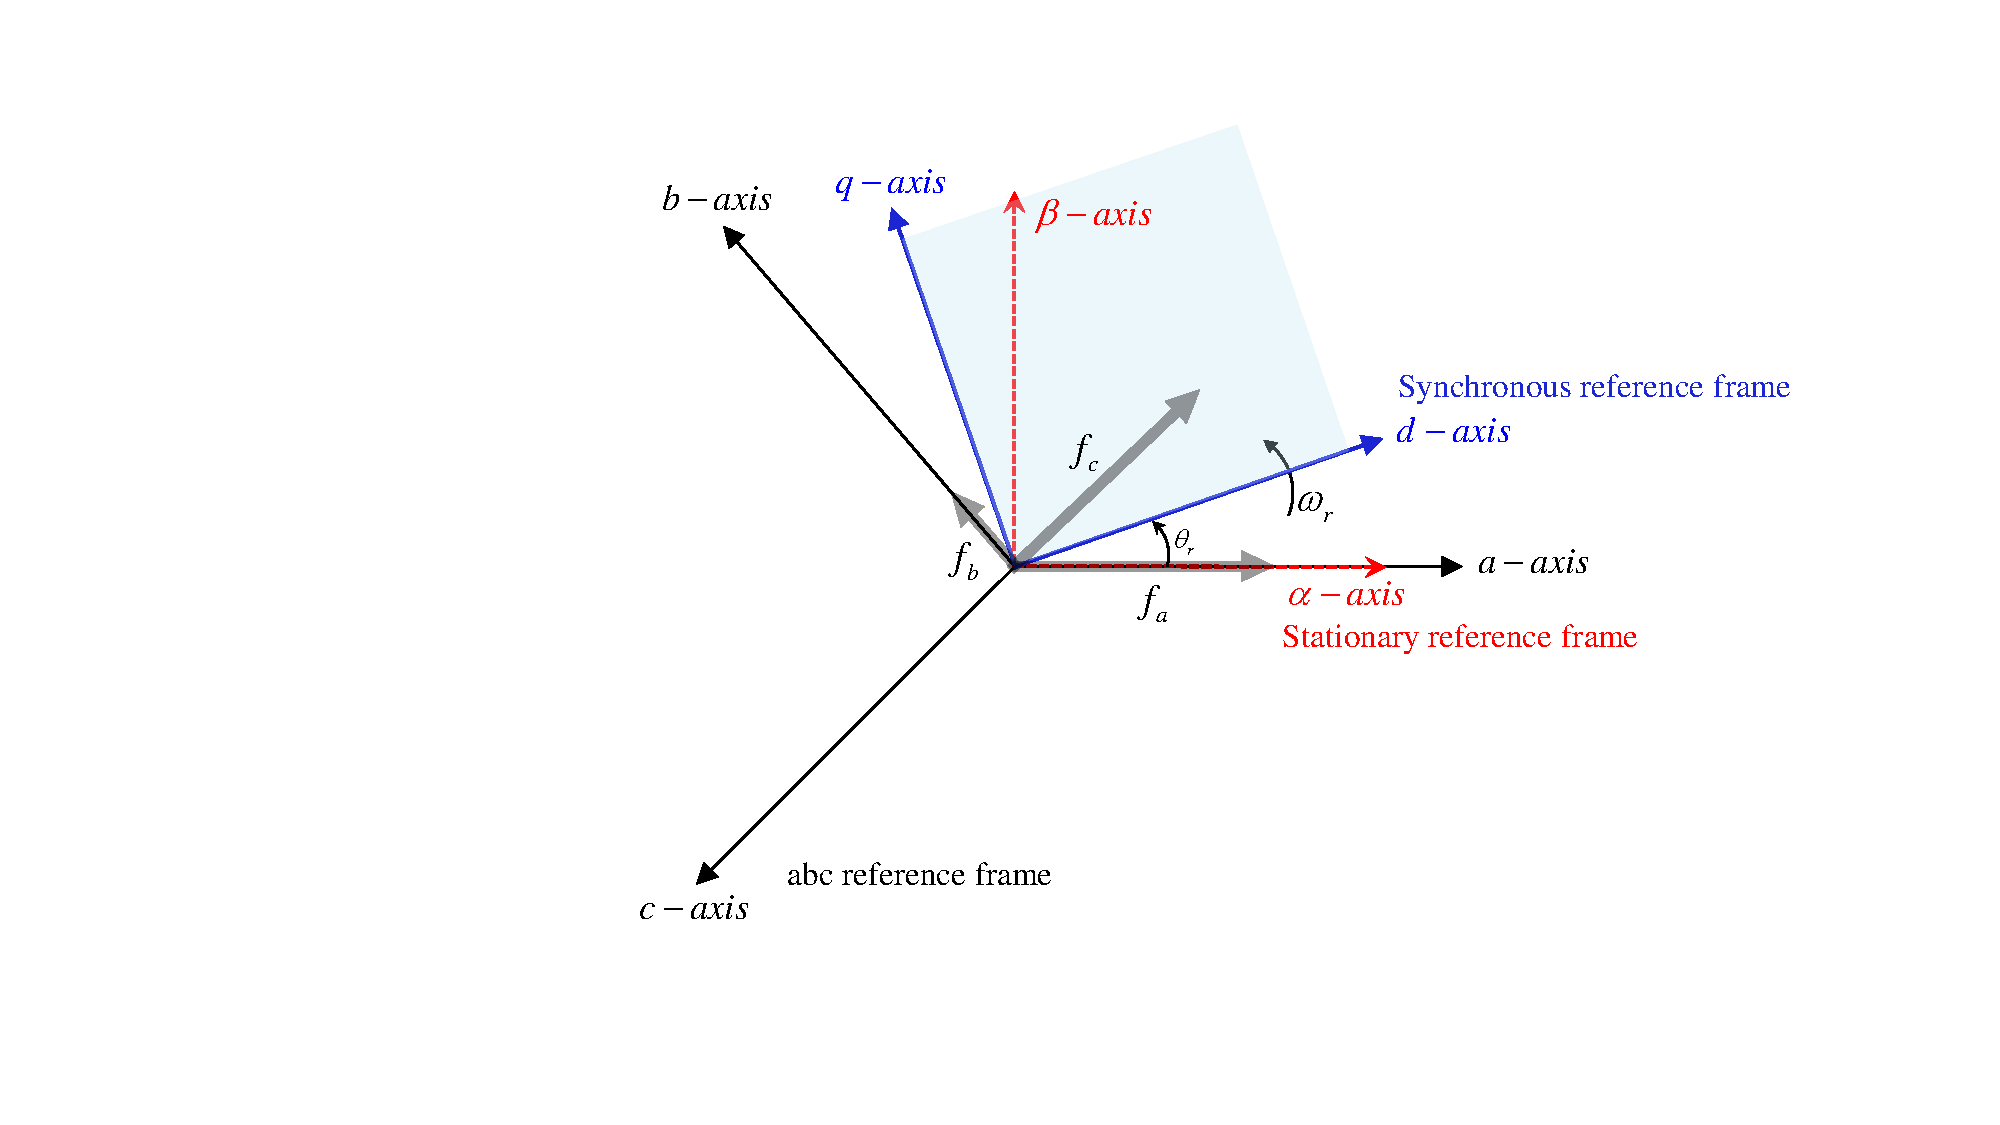
\includegraphics[scale=0.6]{chapters/Fig2.3.pdf}
    \caption{($a$,$b$,$c$)-reference frame, stationary ($\alpha$,$\beta$)-reference frame and rotating ($d$,$q$)-reference frame.}
    \label{Fig:2.3}
\end{figure}

\subsubsection{Modeling in the stationary  ($\alpha$,$\beta$)-reference frame}
The machine model (\ref{eqn:2.2}) can be expressed in the stationary ($\alpha$,$\beta$)-reference frame with orthogonal $\alpha$- and $\beta$-axes, where the zero-sequence component can be neglected due to the balanced three-phase signals in (\ref{eqn:2.1}). Such stator-fixed reference frame transformation for balanced signals can be simplified by using the transformation matrix
\begin{equation}\label{eqn:2.4}
\mathbf{T}(0) := \underbrace{\frac{2}{3} \begin{bmatrix}
1 & -\frac{1}{2} & -\frac{1}{2} \\
0 & \frac{\sqrt{3}}{2} & -\frac{\sqrt{3}}{2}\\
\frac{1}{2} & \frac{1}{2} & \frac{1}{2}
\end{bmatrix}}_{\mathbf{T}(0)\in \mathbb{R}^{3\times3}} \Rightarrow 
\mathbf{T}_c := \underbrace{\frac{2}{3} \begin{bmatrix}
1 & -\frac{1}{2} & -\frac{1}{2} \\
0 & \frac{\sqrt{3}}{2} & -\frac{\sqrt{3}}{2} 
\end{bmatrix}}_{\mathbf{T}_c\in \mathbb{R}^{2\times3}},
\end{equation}
where $\mathbf{T}(0)$ is called the \emph{Clarke transformation matrix} and $\mathbf{T}_c$ represents the \emph{simplified Clarke transformation matrix}, where the last row in $\mathbf{T}(0)$ can be neglected for balanced signals (see Chap.14 in \cite{c2.1_3}), reducing the three-phase signal vectors to two. By introducing the transformed quantities 
\begin{equation}\notag
\bm{u}_s^{\alpha\beta} := \mathbf{T}_c \bm{u}_s^{abc}, \quad \bm{i}_s^{\alpha\beta} := \mathbf{T}_c \bm{i}_s^{abc}, \quad \bm{\psi}_s^{\alpha\beta} := \mathbf{T}_c \bm{\psi}_s^{abc} \quad \text{and} \quad \mathbf{T}_c \frac{d}{dt} \bm{\psi}_s^{abc} = \frac{d}{dt} \bm{\psi}_s^{\alpha\beta}
\end{equation}
in the ($\alpha$,$\beta$)-reference frame and the machine dynamics in (\ref{eqn:2.2}) can be expressed as 
\begin{align}\label{eqn:2.5}\notag
\mathbf{u}^{\alpha\beta}_s(t) &= \mathbf{T}_c \mathbf{u}^{abc}_s(t) \\
&= R_s \mathbf{i}^{\alpha\beta}_s(t) + \frac{d}{dt}\underbrace{\bm{\psi}^{\alpha\beta}_s\left(\mathbf{i}^{\alpha\beta}_s(t),\theta_r(t) \right)}_{=:\bm{\psi}^{\alpha\beta}_s(t)},
\end{align}
where $\mathbf{u}^{\alpha\beta}_s := (u^\alpha_s, v^\beta_s)^\top$, $\mathbf{i}^{\alpha\beta}_s := (i^\alpha_s, i^\beta_s)^\top$ and $\bm{\psi}^{\alpha\beta}_s := (\psi^\alpha_s, \psi^\beta_s)^\top$ denote the stator voltage, current and flux linkage vectors in the ($\alpha$,$\beta$)-reference frame, respectively. 

Likewise, applying the simplified clarke transformation in (\ref{eqn:2.4}) to the stator flux linkage vector in (\ref{eqn:2.3}) yields the stator flux linkage vector
\begin{align}\label{eqn:2.7}\notag
\boldsymbol{\psi}^{\alpha\beta}_s\left(\mathbf{i}^{\alpha\beta}_s,\theta_r \right) &= \mathbf{T}_c\boldsymbol{\psi}^{abc}_s\left(\mathbf{i}^{abc}_s,\theta_r \right) \\\notag
&= \underbrace{\mathbf{T}_c\mathbf{L}^{abc}_s(\theta_r)\mathbf{T}^{-1}_c}_{=:\mathbf{L}^{\alpha\beta}_s(\theta_r)\in \mathbb{R}^{2\times2}}\mathbf{i}^{\alpha\beta}_s+\underbrace{\mathbf{T}_c\boldsymbol{\psi}^{abc}_{pm}(\theta_r)}_{=:\boldsymbol{\psi}^{\alpha\beta}_{pm}(\theta_r)\in \mathbb{R}^{2}}
\\
&= \mathbf{L}^{\alpha\beta}_s(\theta_r)\mathbf{i}^{\alpha\beta}_s
+ \boldsymbol{\psi}^{\alpha\beta}_{pm}(\theta_r)
\end{align}
in the ($\alpha$,$\beta$)-reference frame with the transformed stator inductance matrix $\mathbf{L}^{\alpha\beta}_s$ and permanent-magnet flux linkage vector $\boldsymbol{\psi}^{\alpha\beta}_{pm}$
\begin{align}\label{eqn:2.8}
&\hfil \quad \mathbf{L}^{\alpha\beta}_s(\theta_r) := 
\begin{bmatrix}
L_s + \Delta L_s \cos 2\theta_r & -\Delta L_s \sin 2\theta_r \\
-\Delta L_s \sin 2\theta_r & L_s - \Delta L_s \cos 2\theta_r 
  \end{bmatrix}, \boldsymbol{\psi}^{\alpha\beta}_{pm}(\theta_r):=\psi_{pm}\begin{bmatrix}
\cos \theta_r \\
\sin \theta_r 
  \end{bmatrix},
\\
&\hfil \left( L_d := L_{ls} + \frac{3(L_A - L_B)}{2},L_q := L_{ls} + \frac{3(L_A + L_B)}{2}, L_s := \frac{L_d+L_q}{2}, \Delta L_s := \frac{L_d-L_q}{2}\right)\notag
\end{align}
where the coefficients of the $\mathbf{L}^{\alpha\beta}_s$ and $\boldsymbol{\psi}^{\alpha\beta}_{pm}$ vary depending on the rotor positions. Consequently, there are still time-varying coefficients in \(\mathbf{L}^{\alpha\beta}_s\) and machine model (\ref{eqn:2.5}), by applying the rotating ($d$,$q$)-reference frame transformation, which rotates at the synchronous speed with the rotor, the time-varying elements can be eliminated.

\subsubsection{Modeling in the synchronously rotating ($d$,$q$)-reference frame}
The stator-fixed signal vector in the stationary ($\alpha$,$\beta$)-reference frame can be transformed into the synchronously rotating ($d$,$q$)-reference frame with the electrical angle $\theta_r$ by using the simplified transformation matrix
\begin{equation}\label{eqn:2.8}
\mathbf{T}_p(\theta_r) := 
    \underbrace{\begin{bmatrix}
     \cos(\theta_r) & \sin(\theta_r) & 0\\
     -\sin(\theta_r) & \cos(\theta_r) & 0\\
     0 & 0 & 1
    \end{bmatrix}}_{\mathbf{T}_p(\theta_r) \in \mathbb{R}^{3\times3}} \Rightarrow \mathbf{R}(\theta_r) := 
    \underbrace{\begin{bmatrix}
     \cos(\theta_r) & \sin(\theta_r)\\
     -\sin(\theta_r) & \cos(\theta_r)
    \end{bmatrix}}_{\mathbf{R}(\theta_r) \in \mathbb{R}^{2\times2}}, 
\end{equation}
where $\mathbf{T}_p(\theta_r)$ is called the \emph{Park transformation matrix} and $\mathbf{R}(\theta_r)$ represents the \emph{simplified Park transformation matrix}, where the last row and column in $\mathbf{T}_p(\theta_r)$ can be neglected for the balanced signals (see Chap.14 in \cite{c2.1_3}). By introducing the transformed quantities 
\begin{equation}\notag
 \bm{u}_s^{dq} := \mathbf{R}(\theta_r)\bm{u}_s^{\alpha\beta}, \quad \bm{i}_s^{dq} := \mathbf{R}(\theta_r) \bm{i}_s^{\alpha\beta}, \quad \text{and} \quad \bm{\psi}_s^{dq} := \mathbf{R}(\theta_r) \bm{\psi}_s^{\alpha\beta}
\end{equation}
in the ($d$,$q$)-reference frame and the machine dynamics in (\ref{eqn:2.5}) can be expressed as 
\begin{align}\label{eqn:2.9}\notag
\mathbf{u}^{dq}_s(t) &= \mathbf{R}(\theta_r)\mathbf{u}^{\alpha\beta}_s(t) \\\notag
&= R_s\mathbf{i}^{dq}_s(t) + \underbrace{\mathbf{R}(\theta_r)\frac{d\left( \mathbf{R}^{-1}(\theta_r)\boldsymbol{\psi}^{dq}_s\right)}{dt}}_{=:\frac{d}{dt}\boldsymbol{\psi}^{dq}_s + \omega_r \mathbf{J}\boldsymbol{\psi}^{dq}_s} \\
&= R_s \mathbf{i}^{dq}_s(t) +\omega_r(t)\mathbf{J}\boldsymbol{\psi}^{dq}_s(t) + \frac{d}{dt}\underbrace{\boldsymbol{\psi}^{dq}_s\left(\mathbf{i}^{dq}_s(t),\theta_r(t) \right)}_{=:\boldsymbol{\psi}^{dq}_s(t)}, \quad \mathbf{J} :=  
  \begin{bmatrix}
    0 & -1\\1 & 0
  \end{bmatrix}, 
\end{align}
where $\mathbf{u}^{dq}_s := (u^d_s, u^q_s)^\top$, $\mathbf{i}^{dq}_s := (i^d_s, i^q_s)^\top$ and $\boldsymbol{\psi}^{dq}_s := (\psi^d_s, \psi^q_s)^\top$ denote the stator voltage, current, and flux linkage vectors in the ($d$,$q$)-reference frame, where all physical variables become constant with respect to time. $\omega_r$ represents the electrical velocity of the rotor.

Similarly, applying the simplified Park transformation in (\ref{eqn:2.8}) to the stationary reference frame flux linkage in  (\ref{eqn:2.7}) results the stator flux linkage vector
\begin{align}\notag
\boldsymbol{\psi}^{dq}_s(\mathbf{i}^{dq}_s) 
&=\underbrace{\mathbf{R}(\theta_r)\mathbf{L}^{\alpha\beta}_s(\theta_r)\mathbf{R}(\theta_r)^{-1}}_{=:\mathbf{L}^{dq}_s(\mathbf{i}^{dq}_s)=\mathbf{L}^{dq}_s(t)}\mathbf{i}^{dq}_s
+ \underbrace{\mathbf{R}(\theta_r)\boldsymbol{\psi}^{\alpha\beta}_{pm}(\theta_r)}_{=:\boldsymbol{\psi}^{dq}_{pm}(\mathbf{i}^{dq}_s)=\boldsymbol{\psi}^{dq}_{pm}(t)}
\\\label{eqn:2.10}
&= \mathbf{L}^{dq}_s(\mathbf{i}^{dq}_s)\mathbf{i}^{dq}_s + \boldsymbol{\psi}^{dq}_{pm}(\mathbf{i}^{dq}_s),
\end{align}
in the ($d$,$q$)-reference frame with the static inductance matrix $\mathbf{L}^{dq}_s$ considering the cross-coupling effects and magnetic saturation \cite{c2.1_2} and permanent-magnet flux linkage vector $\boldsymbol{\psi}^{dq}_{pm}$ 
\begin{align}\label{eqn:2.11}
\mathbf{L}^{dq}_s(\mathbf{i}^{dq}_s) = \begin{bmatrix}
L^d_s(i^d_s,i^q_s) & 0 \\
0 & L^q_s(i^d_s,i^q_s) \\
\end{bmatrix}, \quad {\boldsymbol{\psi}^{dq}_{pm} = \psi_{pm}(i^d_s,i^q_s) \begin{bmatrix}
1 \\
0
\end{bmatrix}}.
\end{align}
Due to the choice of $\theta_r(\cdot)$ in (\ref{eqn:2.8}) (i.e., the so-called permanent-magnet flux linkage orientation or, simply, field orientation), the stator flux linkage vector $\bm{\psi}^{dq}_s(\bm{i}^{dq}_s)$ does not depend on the electrical or the mechanical angle anymore (constant). Moreover, the permanent-magnet flux linkage simplifies to the constant $d$-component $\psi_{pm}$. Figure \ref{Fig:2.4} shows an example of the static inductances ($L^d_s$, $L^q_s$) and the permanent magnet flux linkage ($\psi_{pm}$) for the $d$- and $q$-axis currents of an IPMSM obtained through extensive experiments.

In general, the flux linkage vector in (\ref{eqn:2.10}) can be expressed as a linear relationship between the $d$- and $q$-axis stator currents, the constant inductances ($L^d_s$, $L^q_s$), and the permanent magnet flux linkage ($\psi_{pm}$), when the stator currents are small. Thus, substituting (\ref{eqn:2.10}) for the constant parameters into (\ref{eqn:2.9}) leads the current dynamics as scalar equations, i.e.
\begin{align}\label{eqn:2.12}
L^d_s \frac{d}{dt}i^d_s(t) &= -R_s i^d_s(t) + \omega_r(t) L^q_s i^q_s(t) + u^d_s(t), \\\label{eqn:2.13}
L^q_s \frac{d}{dt}i^q_s(t) &= -R_s i^q_s(t) - \omega_r(t) (L^d_s i^d_s(t) + \psi_{pm}) + u^q_s(t).
\end{align}

Accordingly, the machine torque 
\begin{align}\notag
T_e(\mathbf{i}^{dq}_s,\bm{\psi}^{dq}_{s}) &= \frac{3}{2}n_p \bm{\psi}^{dq}_{s}(\mathbf{i}^{dq}_s) \times \bm{i}^{dq}_s \\\label{eqn:2.14}
&= \frac{3}{2}n_p  \left( \psi_{pm} + (L^d_s - L^q_s) i^d_s\right)i^q_s
\end{align}
in the ($d$,$q$)-reference frame can be derived. 

\begin{figure}[t]
    \centering
    \begin{subfigure}[b]{0.30\textwidth}
        \centering
        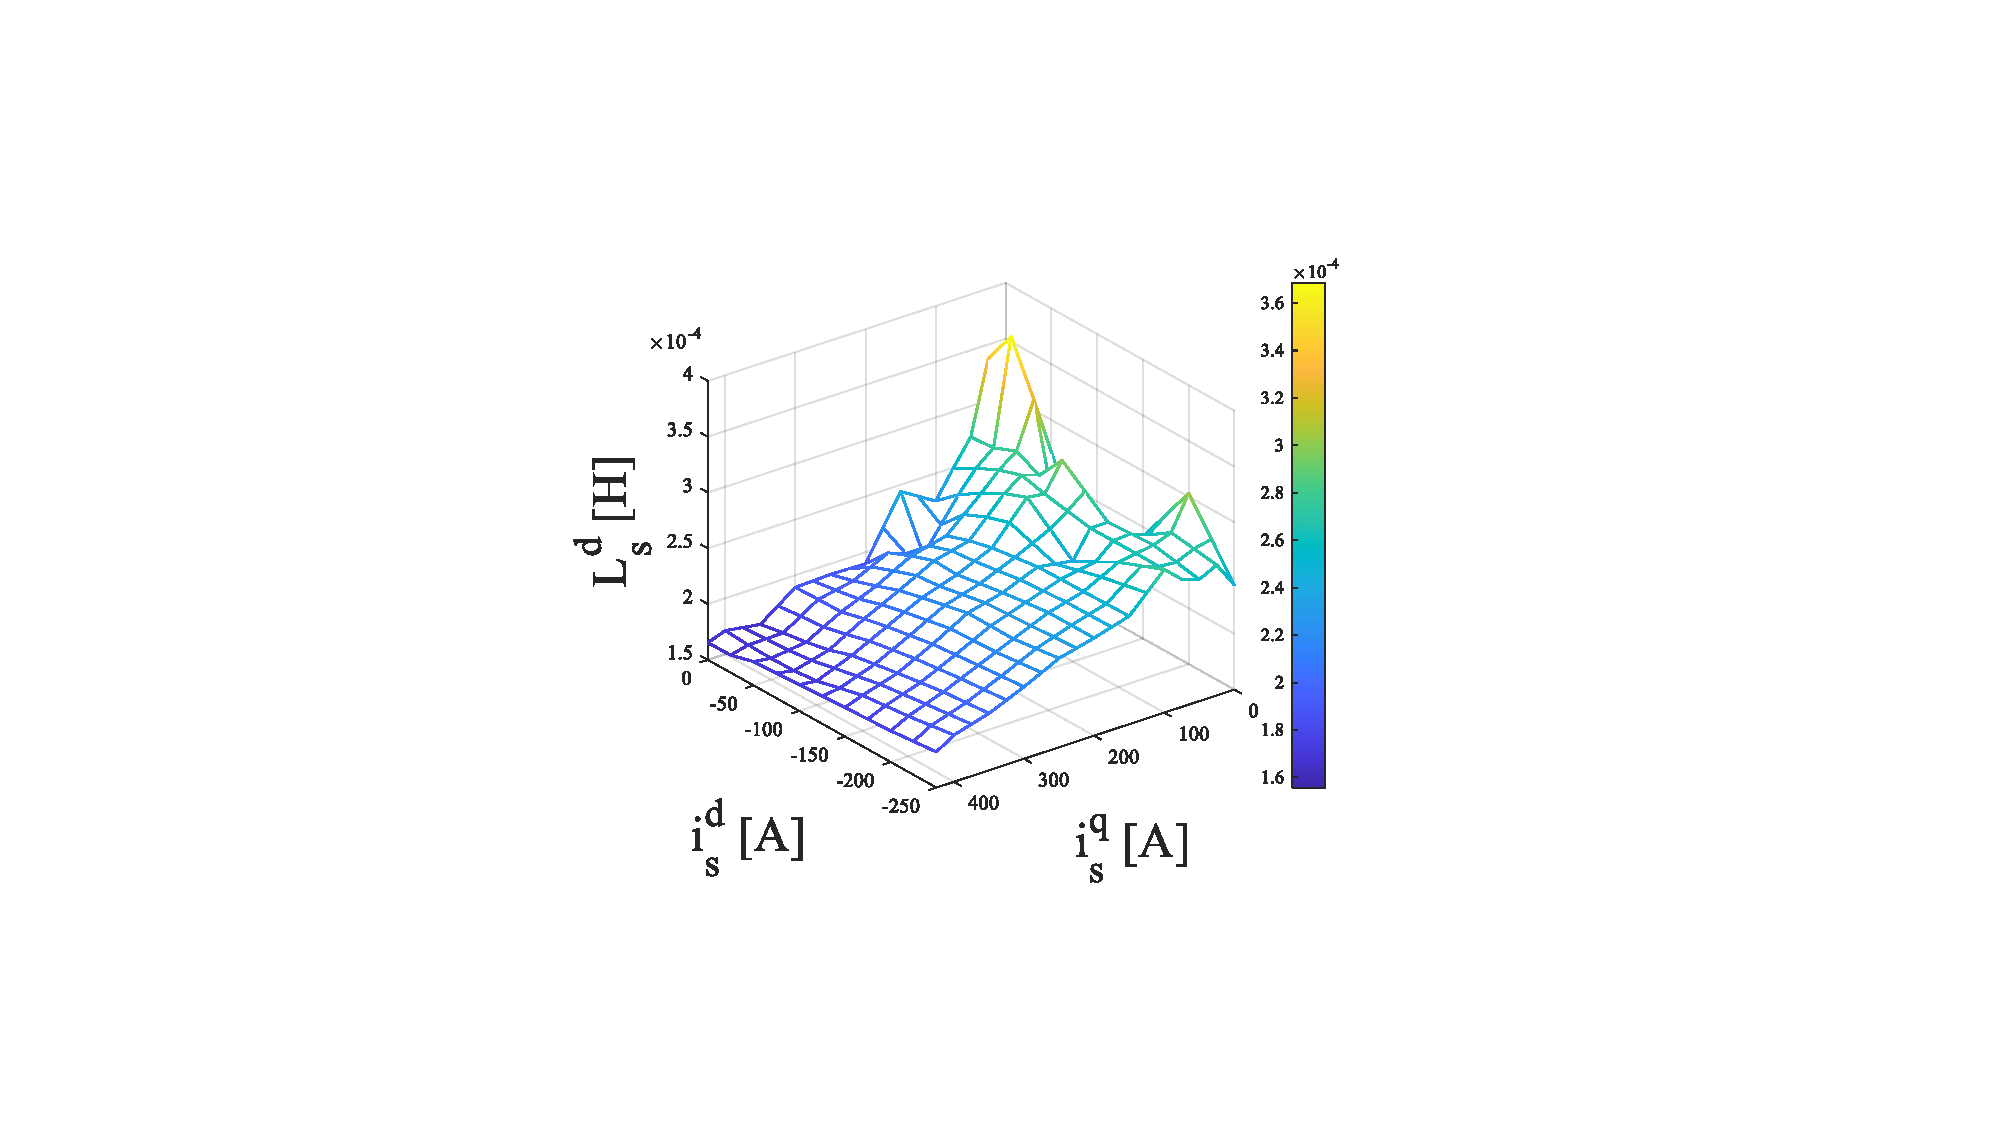
\includegraphics[scale=0.4]{chapters/Fig2.4a.pdf}
        \caption{}
        \label{Fig:2.4a}
    \end{subfigure}
    \hfill
    \begin{subfigure}[b]{0.30\textwidth}
        \centering
        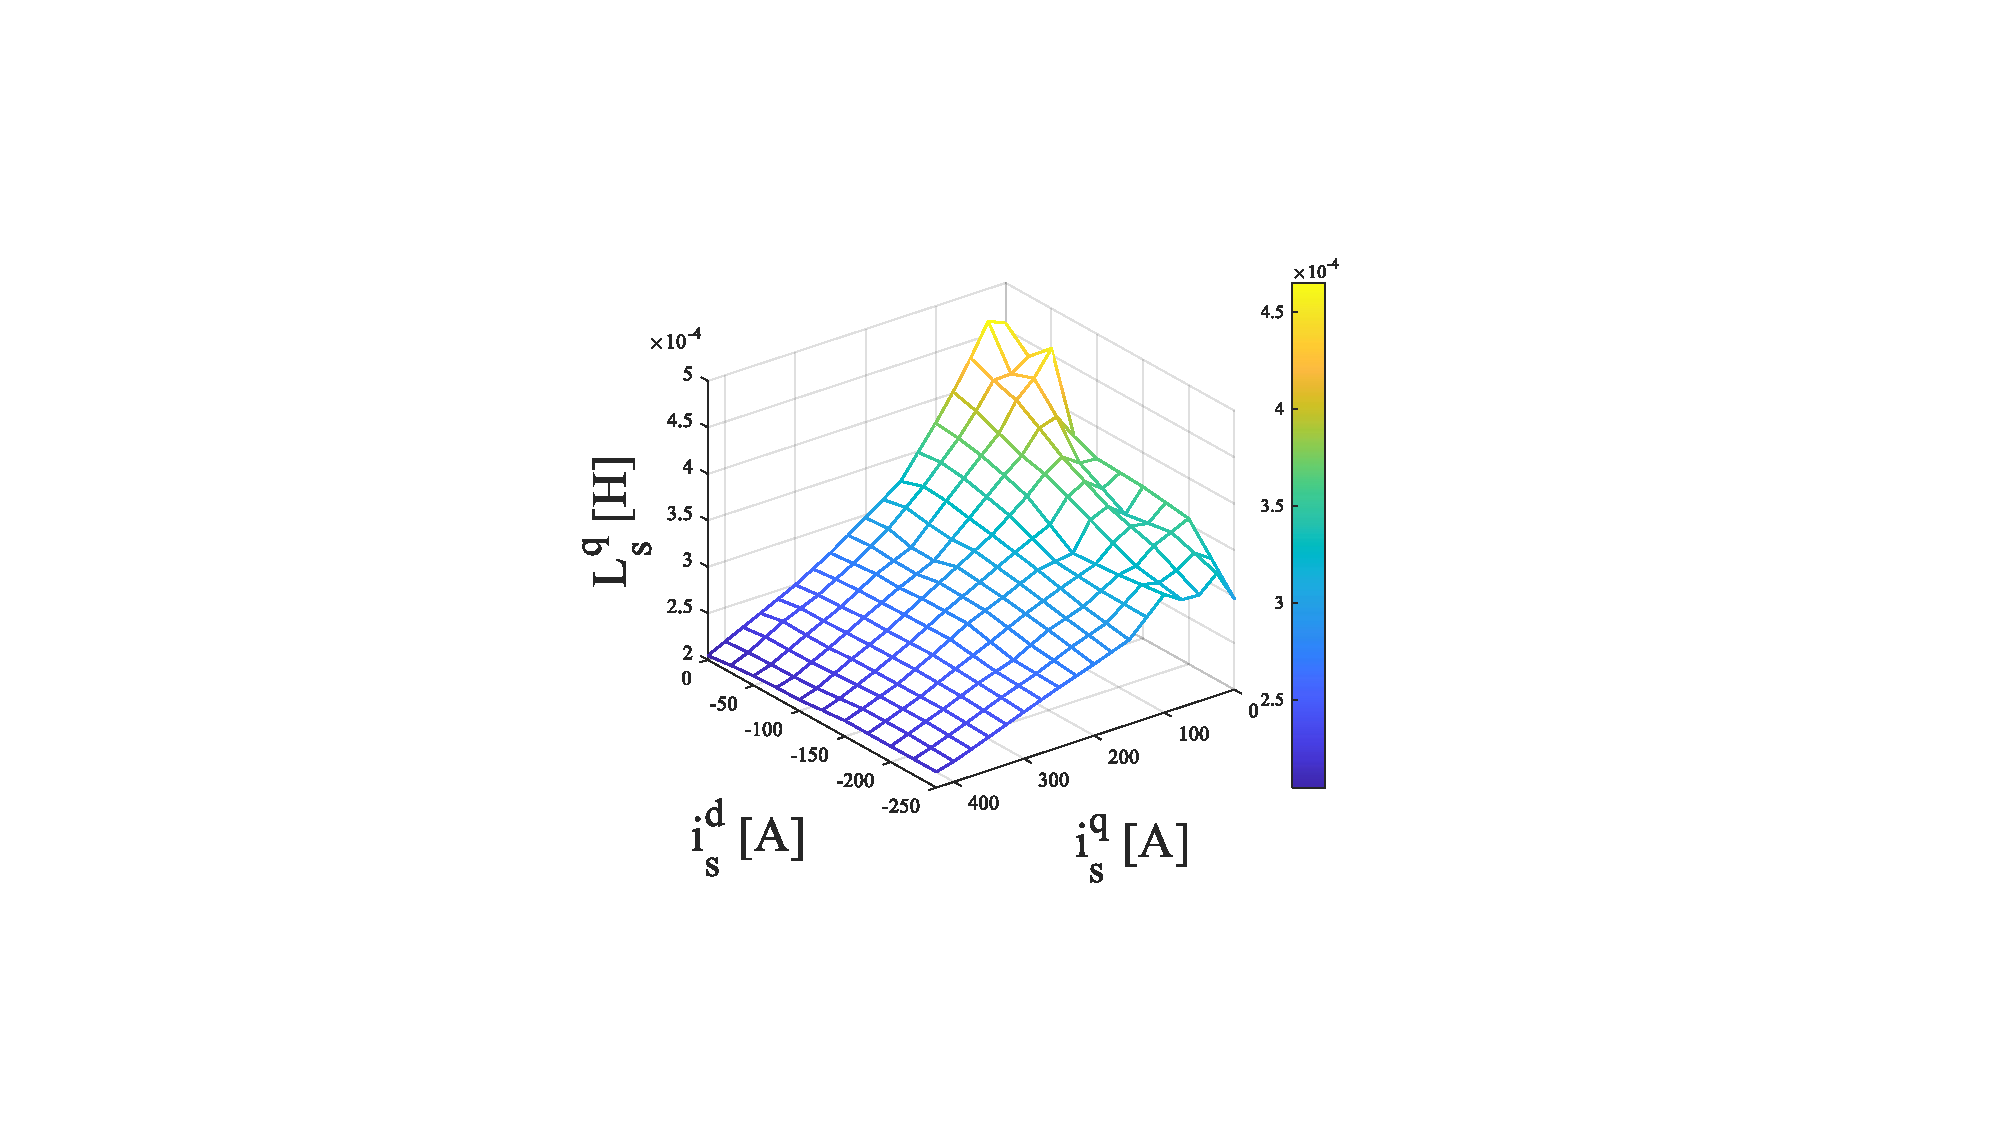
\includegraphics[scale=0.4]{chapters/Fig2.4b.pdf}
        \caption{}
        \label{Fig:2.4b}
    \end{subfigure}
    \hfill
    \begin{subfigure}[b]{0.30\textwidth}
        \centering
        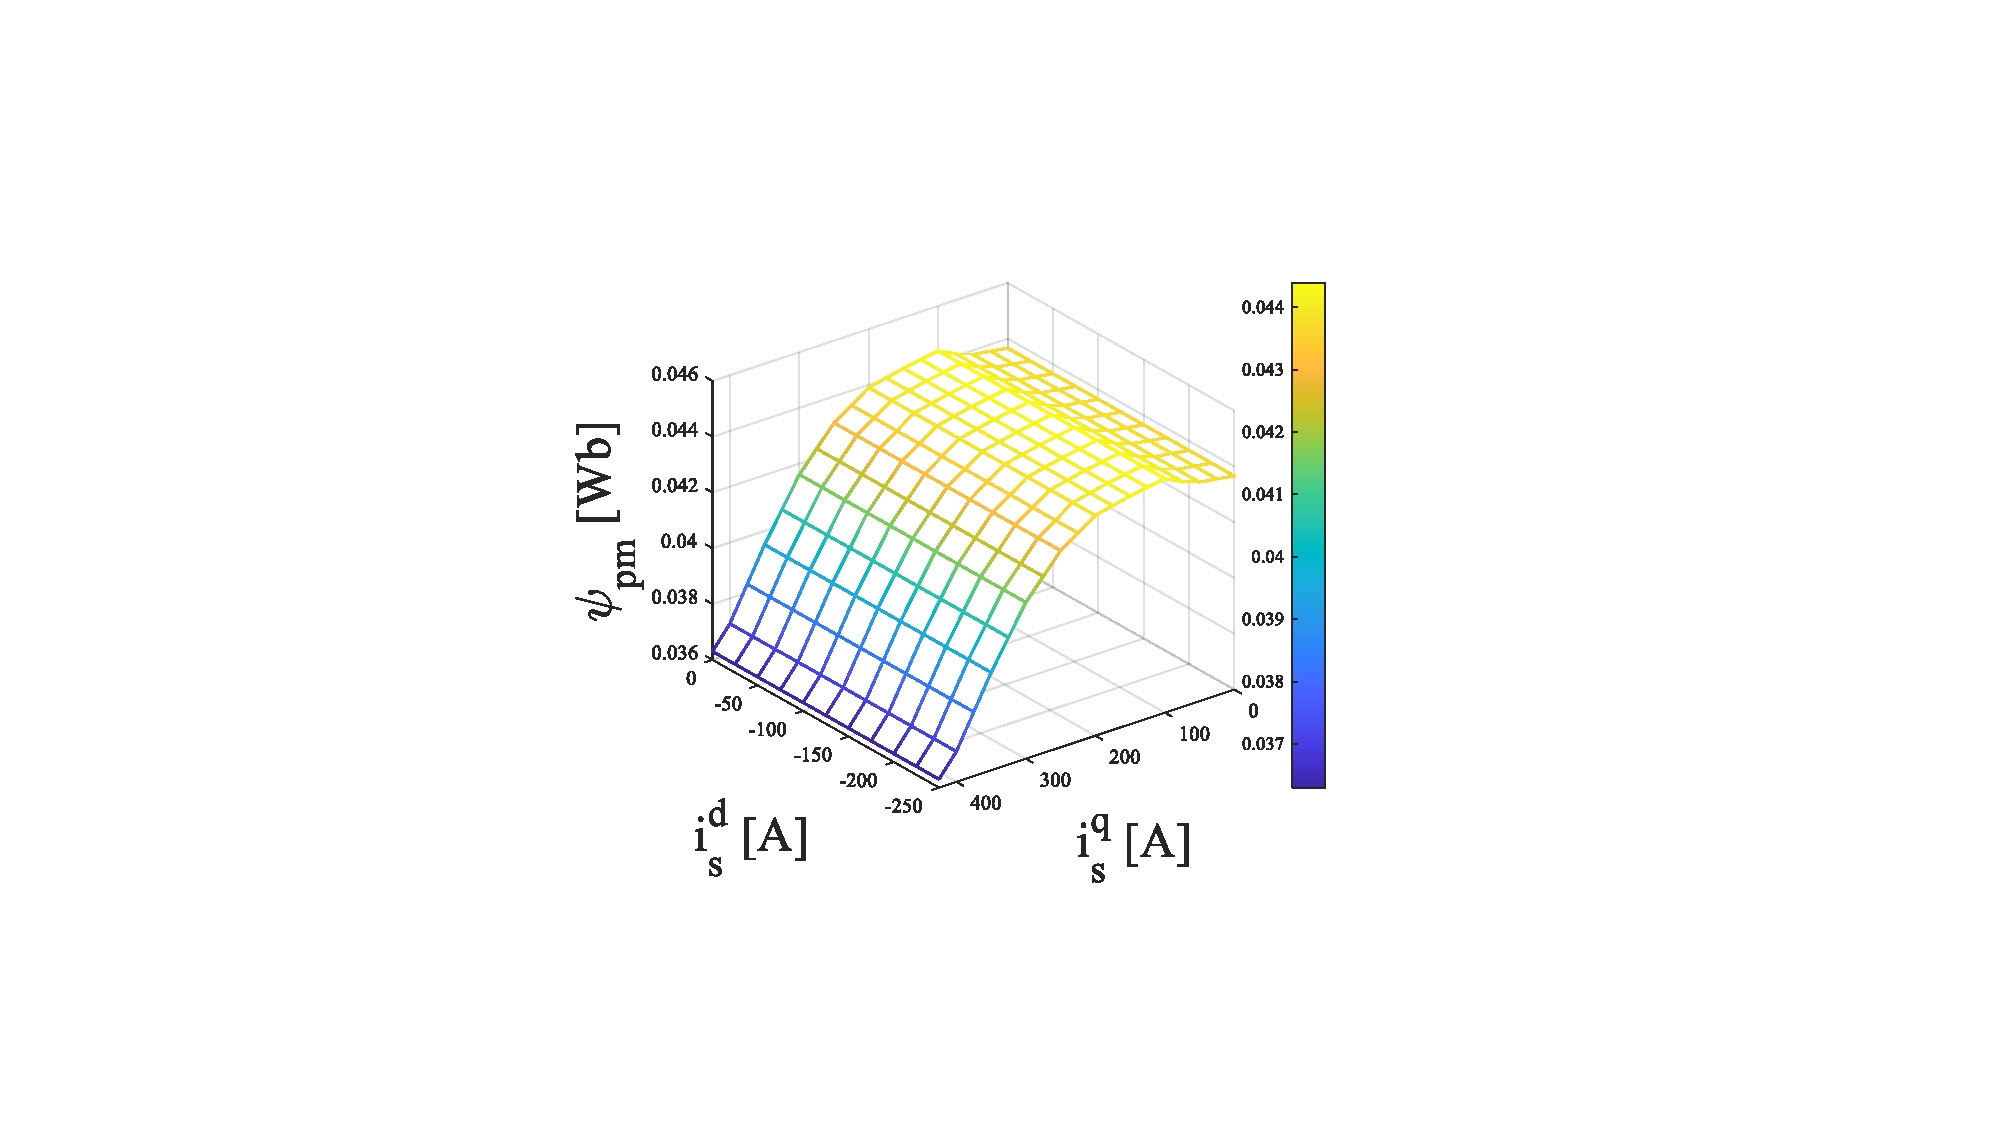
\includegraphics[scale=0.4]{chapters/Fig2.4c.pdf}
        \caption{}
        \label{Fig:2.4c}
    \end{subfigure}
    \caption{Stator inductance and permanent magnetic flux linkage of a PMSM versus $d-$ and $q$-axes currents. (a) d-axis inductance. (b) q-axis inductance. (c) permanent magnetic flux linkage.}
    \label{Fig:2.4}
\end{figure}

Practically, the machine parameters ($L^d_s$, $L^q_s$, $\psi_{pm}$) are highly influenced by the temperature of the cores (stator, rotor), permanent magnets in the rotor and stator winding, which degrades the permeability of the cores and reduces their ability to magnetize \cite{k1},\cite{k2}. Ultimately, due to continuous changes in parameters caused not only by the behavior of the stator current but also by temperature variations in the rotor and stator windings, it is necessary to develop methods for online estimation of these parameters to improve the operating performance of the SMs.

\section{Optimal Control Strategy for SM}\label{chap2:2.2} 
Model Predictive Control (MPC) offers a more flexible optimal control solution compared to conventional feedforward-based PI regulators that determine the switch mode operation of power switch devices through PWM (Pulse Width Modulation), by evaluating an appropriate cost function that allows to selection of the possible switching states as control inputs from either a Continuous Control Set (CCS) or a Finite Control Set (FCS). This approach offers the advantage of optimizing several control conditions such as switching frequency, switching losses, and machine torque ripple minimization while considering the constraints of the SM. However, to achieve these optimizations, a significant computation burden is required, especially because the CCS-MPC method determines control inputs within a continuous control set range, necessitating complex and computationally intensive optimization \cite{c2.2_5},\cite{c2.2_6}. In contrast, the FCS-MPC method considers control inputs within a finite control set, simplifying the optimization process and reducing the computational burden compared to CCS-MPC. Moreover, FCS-MPC has the advantages of intuitive concept, easy handling of nonlinear constraints, and realization of multivariable control \cite{c2.2_1},\cite{c2.2_2}.
Additionally, the calculation burden of the optimal solutions for MPC-based methods has been improved by the development of cost-effective and efficient microprocessors, allowing for extensive computations at low cost \cite{c2.2_3}. Therefore, with accurate parameter information of the SMs model, the FCS-MPC method is an excellent alternative to PI regulator. This section focuses on introducing the FCS-MPC method for the current control of IPMSM.

\subsubsection{Finite Control Set Model Predictive Current Control} \label{sec2:2-2}
Finite Control Set Model Predictive Current Control (FCS-MPCC) is an FCS-MPC-based optimal current control method that defines the objective function as the error between the predicted current and the reference current, based on discrete-time model dynamics. The switching states (one of the eight switching states of a 2-level inverter) corresponding to the minimum value of this objective function are determined as the control inputs. Therefore, it has the advantage of easily designing and evaluating objective functions to optimize control conditions such as switching and power loss minimization while considering the voltage and current limits of the synchronous machine.

Typically, to obtain the predicted currents, the derivative of the $d$-$q$ axis currents with respect to discrete time can be expressed using a \emph{forward Euler approximation} \cite{c2.2_3} as follows.
\begin{equation}\label{eqn:2.15}
\frac{d\mathbf{i}^{dq}_s}{dt} \approx \frac{\mathbf{i}^{dq}_s(k+1) - \mathbf{i}^{dq}_s(k)}{T_s},
\end{equation}
Here, \( T_s \) is the sampling time. 

By substituting the discrete-time current dynamics in (\ref{eqn:2.15}) into the scalar equations (\ref{eqn:2.12}) and (\ref{eqn:2.13}) respectively, the prediction of the future currents in the ($d$,$q$)-reference frame at the \( k+1 \) time can be expressed as 
\begin{align}\label{eqn:2.16}
i^{d,p}_s(k + 1) &= \left( 1 - \frac{R_s T_s}{L^d_s} \right) i^{d}_s(k) + \frac{T_s}{L^d_s}\left( \omega_r(k) L^q_s i^{q}_s(k) + {u_{s}^q}^*(k)  \right),  \\\label{eqn:2.17} 
i^{q,p}_s(k + 1) &= \left( 1 - \frac{R_s T_s}{L^q_s} \right) i^{q}_s(k) - \frac{T_s}{L^q_s}\left( \omega_r(k) L^d_s i^d_s(k) + \omega_r(k) \psi_{pm}  - {u_{s}^d}^*(k) \right),
\end{align}
where $i^{d,p}_s$ and $i^{q,p}_s$ represent the predicted $d$- and $q$-axis stator currents. Here, the possible voltage references in the ($d$,$q$)-reference frame as control inputs (${u_{s}^d}^*$,${u_{s}^q}^*$) are composed of a finite control set (8 switching states). Accordingly, to determine the control inputs (${u_{s}^d}^*$,${u_{s}^q}^*$), the three-phase voltage references in the ($a$,$b$,$c$)-reference frame can be expressed using the switching functions as follows
\begin{align}\label{eqn:2.18}
{u_{s}^a}^*(n) &= \frac{U_{dc}}{3}\left(2S_a(n) - S_b(n) - S_c(n)\right), \\\label{eqn:2.19}
{u_{s}^b}^*(n) &= \frac{U_{dc}}{3}\left(2S_b(n) - S_a(n) - S_c(n)\right), \\\label{eqn:2.20}
{u_{s}^c}^*(n) &= \frac{U_{dc}}{3}\left(2S_c(n) - S_b(n) - S_a(n)\right), \\
\bm{S}(n) &= \left(S_a(n),S_b(n),S_c(n)  \right), 
\end{align}
where \( U_{dc} \) is the input voltage, and \( {u_{s}^a}^* \), \( {u_{s}^b}^* \), and \( {u_{s}^c}^* \) denote the voltage references in the ($a$,$b$,$c$)-reference frame, respectively. \( S_a \), \( S_b \), and \( S_c \) represent the switching states of each phase, where $1$ indicates the switch is ON and $0$ indicates the switch is OFF, operating complementarily within each phase's switch leg and \(\bm{S}\) denotes the switching state vector, including each phase. Table \ref{Table:2.1} and Fig.\ref{Fig:2.8} show all possible combinations of the switching states, space voltage vectors, and cost functions. 

\begin{table}[t]
\centering
\setlength{\tabcolsep}{5pt}
\begin{tabular}{    c|
    c|
    c|c|c|c
}
\toprule
\hline
\multicolumn{1}{c|}{Cost Function} & \multicolumn{1}{c|}{Switching States} & \multicolumn{3}{c}{Phase Voltages} & \multicolumn{1}{|c}{Space Voltage Vectors} \\
\hline
$g$ &$\mathbf{S}(n)$ = ($S_a$,$S_b$,$S_c$) & $u^a_{s}$ & $u^b_{s}$ & $u^c_{s}$ & $\mathbf{U}_n(n =0-7)$\\  
\hline
$g_0$ & $\mathbf{S}(0)$ = ($0$,$0$,$0$) & $0$ & $0$ & $0$ & $\mathbf{U}_0 =0\angle 0^\circ$ \\
$g_1$ &  $\mathbf{S}(1)$ = ($1$,$0$,$0$) & $\frac{2}{3}U_{dc}$ & $-\frac{1}{3}U_{dc}$ & $-\frac{1}{3}U_{dc}$ & $\mathbf{U}_1 =\frac{2}{3}U_{dc}\angle 0^\circ$\\
$g_2$ &  $\mathbf{S}(2)$ = ($1$,$1$,$0$) & $\frac{1}{3}U_{dc}$ & $\frac{1}{3}U_{dc}$ & $-\frac{2}{3}U_{dc}$ & $\mathbf{U}_2 =\frac{2}{3}U_{dc}\angle 60^\circ$\\
$g_3$ & $\mathbf{S}(3)$ = ($0$,$1$,$0$) & $-\frac{1}{3}U_{dc}$ & $\frac{2}{3}U_{dc}$ & $-\frac{1}{3}U_{dc}$ & $\mathbf{U}_3 =\frac{2}{3}U_{dc}\angle 120^\circ$ \\
$g_4$ & $\mathbf{S}(4)$ = ($0$,$1$,$1$) & $-\frac{2}{3}U_{dc}$ & $\frac{1}{3}U_{dc}$ & $\frac{1}{3}U_{dc}$ & $\mathbf{U}_4 =\frac{2}{3}U_{dc}\angle 180^\circ$ \\
$g_5$ & $\mathbf{S}(5)$ = ($0$,$0$,$1$) & $-\frac{1}{3}U_{dc}$ & $-\frac{1}{3}U_{dc}$ & $\frac{2}{3}U_{dc}$ & $\mathbf{U}_5 =\frac{2}{3}U_{dc}\angle 240^\circ$\\
$g_6$ &  $\mathbf{S}(6)$ = ($1$,$0$,$1$) & $\frac{1}{3}U_{dc}$ & $-\frac{2}{3}U_{dc}$ & $\frac{1}{3}U_{dc}$ & $\mathbf{U}_6 =\frac{2}{3}U_{dc}\angle 300^\circ$\\
$g_7$ &  $\mathbf{S}(7)$ = ($1$,$1$,$1$) & $0$ & $0$ & $0$ & $\mathbf{U}_7 =0\angle 0^\circ$\\
\hline
\bottomrule
\end{tabular}
\caption{Switching states, phase 
 voltages and space voltage vector with a cost function.}\label{Table:2.1}
\end{table}
\begin{figure}[t]
    \centering
    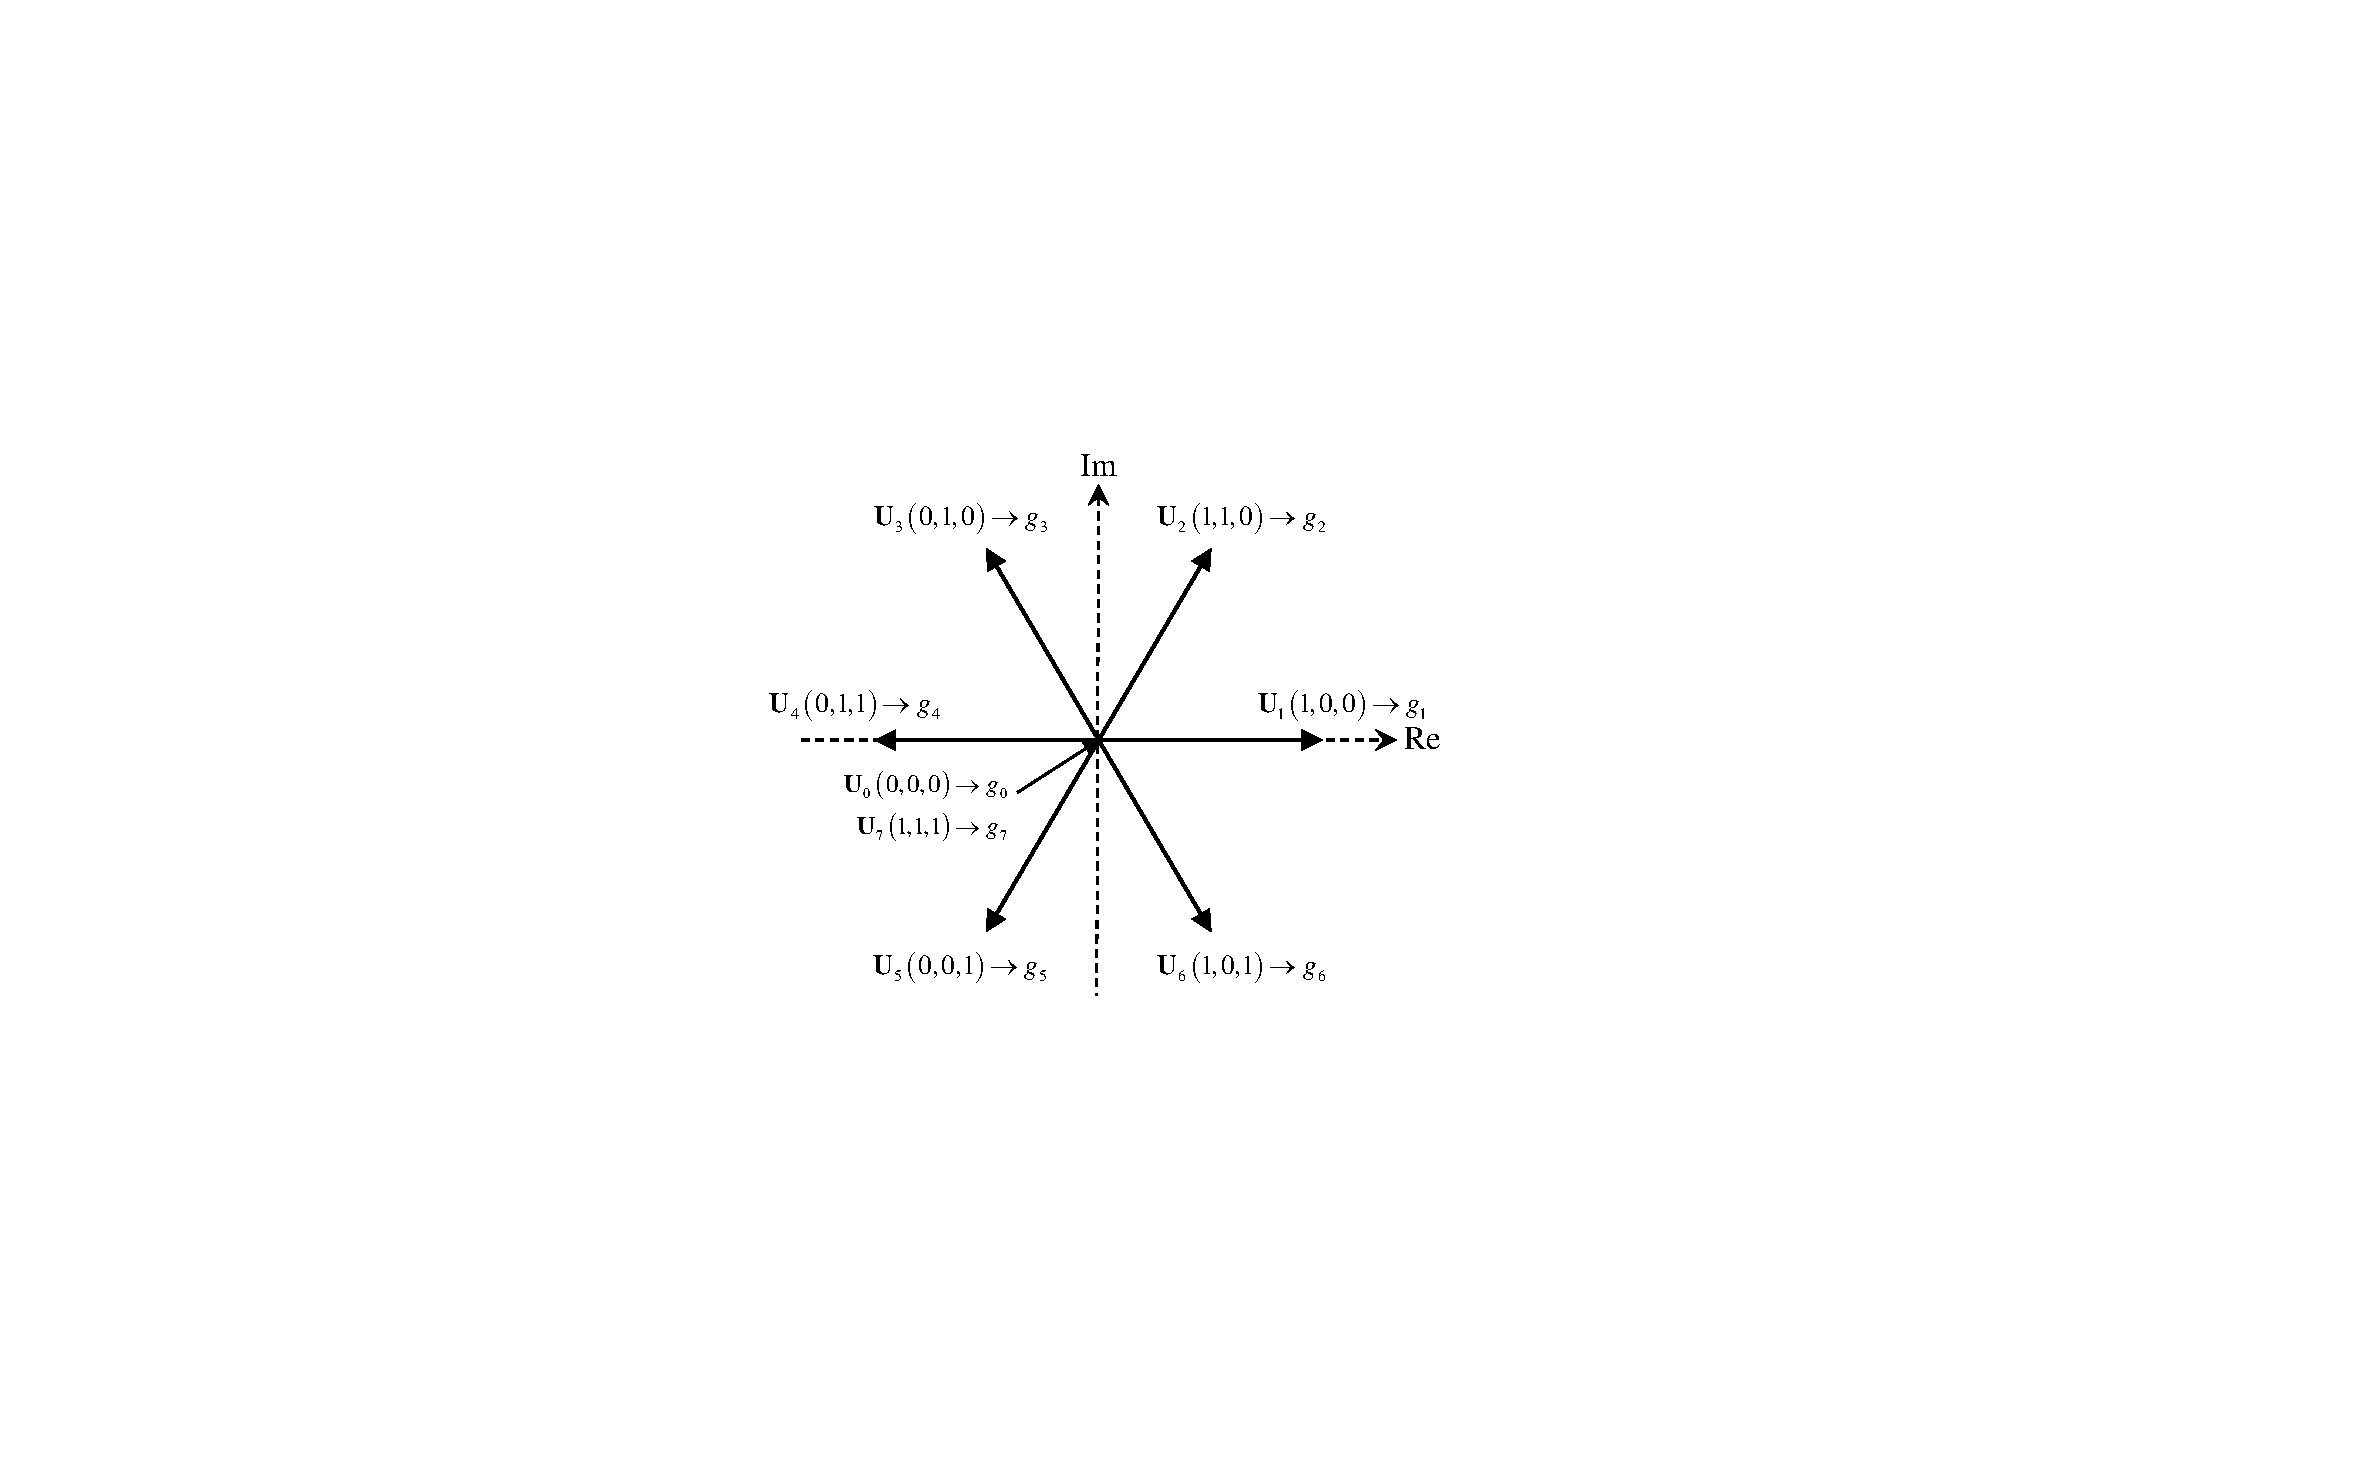
\includegraphics[scale=0.70]{chapters/Fig2.8.pdf}
    \caption{Voltage vectors and corresponding cost function in the complex plane.}
    \label{Fig:2.8}
\end{figure}

Transforming the voltage references in the ($a$,$b$,$c$)-reference frame (${u_{s}^a}^*$,${u_{s}^b}^*$,${u_{s}^c}^*$) to the ($d$,$q$)-reference frame (${u_{s}^d}^*$,${u_{s}^q}^*$) results as follows
\begin{align}\label{eqn:2.22}
{u_{s}^d}^*(k) &= \frac{2}{3} \left( {u_{s}^a}^* \cos\left(\theta_r\right) + {u_{s}^b}^* \cos\left(\theta_r - \frac{2\pi}{3}\right) + {u_{s}^c}^* \cos\left(\theta_r + \frac{2\pi}{3}\right) \right), \\\label{eqn:2.23}
{u_{s}^q}^*(k) &= -\frac{2}{3} \left( {u_{s}^a}^* \sin\left(\theta_r\right) + {u_{s}^b}^* \sin\left(\theta_r - \frac{2\pi}{3}\right) + {u_{s}^c}^* sin\left(\theta_r + \frac{2\pi}{3}\right) \right),
\end{align}
whereby substituting the voltage references in (\ref{eqn:2.22}) and (\ref{eqn:2.23}) calculated from the three-phase stator voltage references (${u_{s}^a}^*$,${u_{s}^b}^*$,${u_{s}^c}^*$) for the 8 switching states into the predicted current dynamics in (\ref{eqn:2.16}) and (\ref{eqn:2.17}), all the predicted currents can be obtained. Therefore, to determine the voltage references in the ($d$,$q$)-reference frame that minimizes the errors between the current references and the predicted currents, the objective function can be derived and evaluated, which the switching state of minimum cost functions $g$ for 8 all switching states are determined as the control input voltages. The operating principle of predictive current control for the implementation is shown in Algorithm \ref{Algorithm:2.1} and Fig \ref{Fig:2.6} shows the control scheme based on the FCS-MPC current controller. 

\begin{figure}[t]
    \centering
    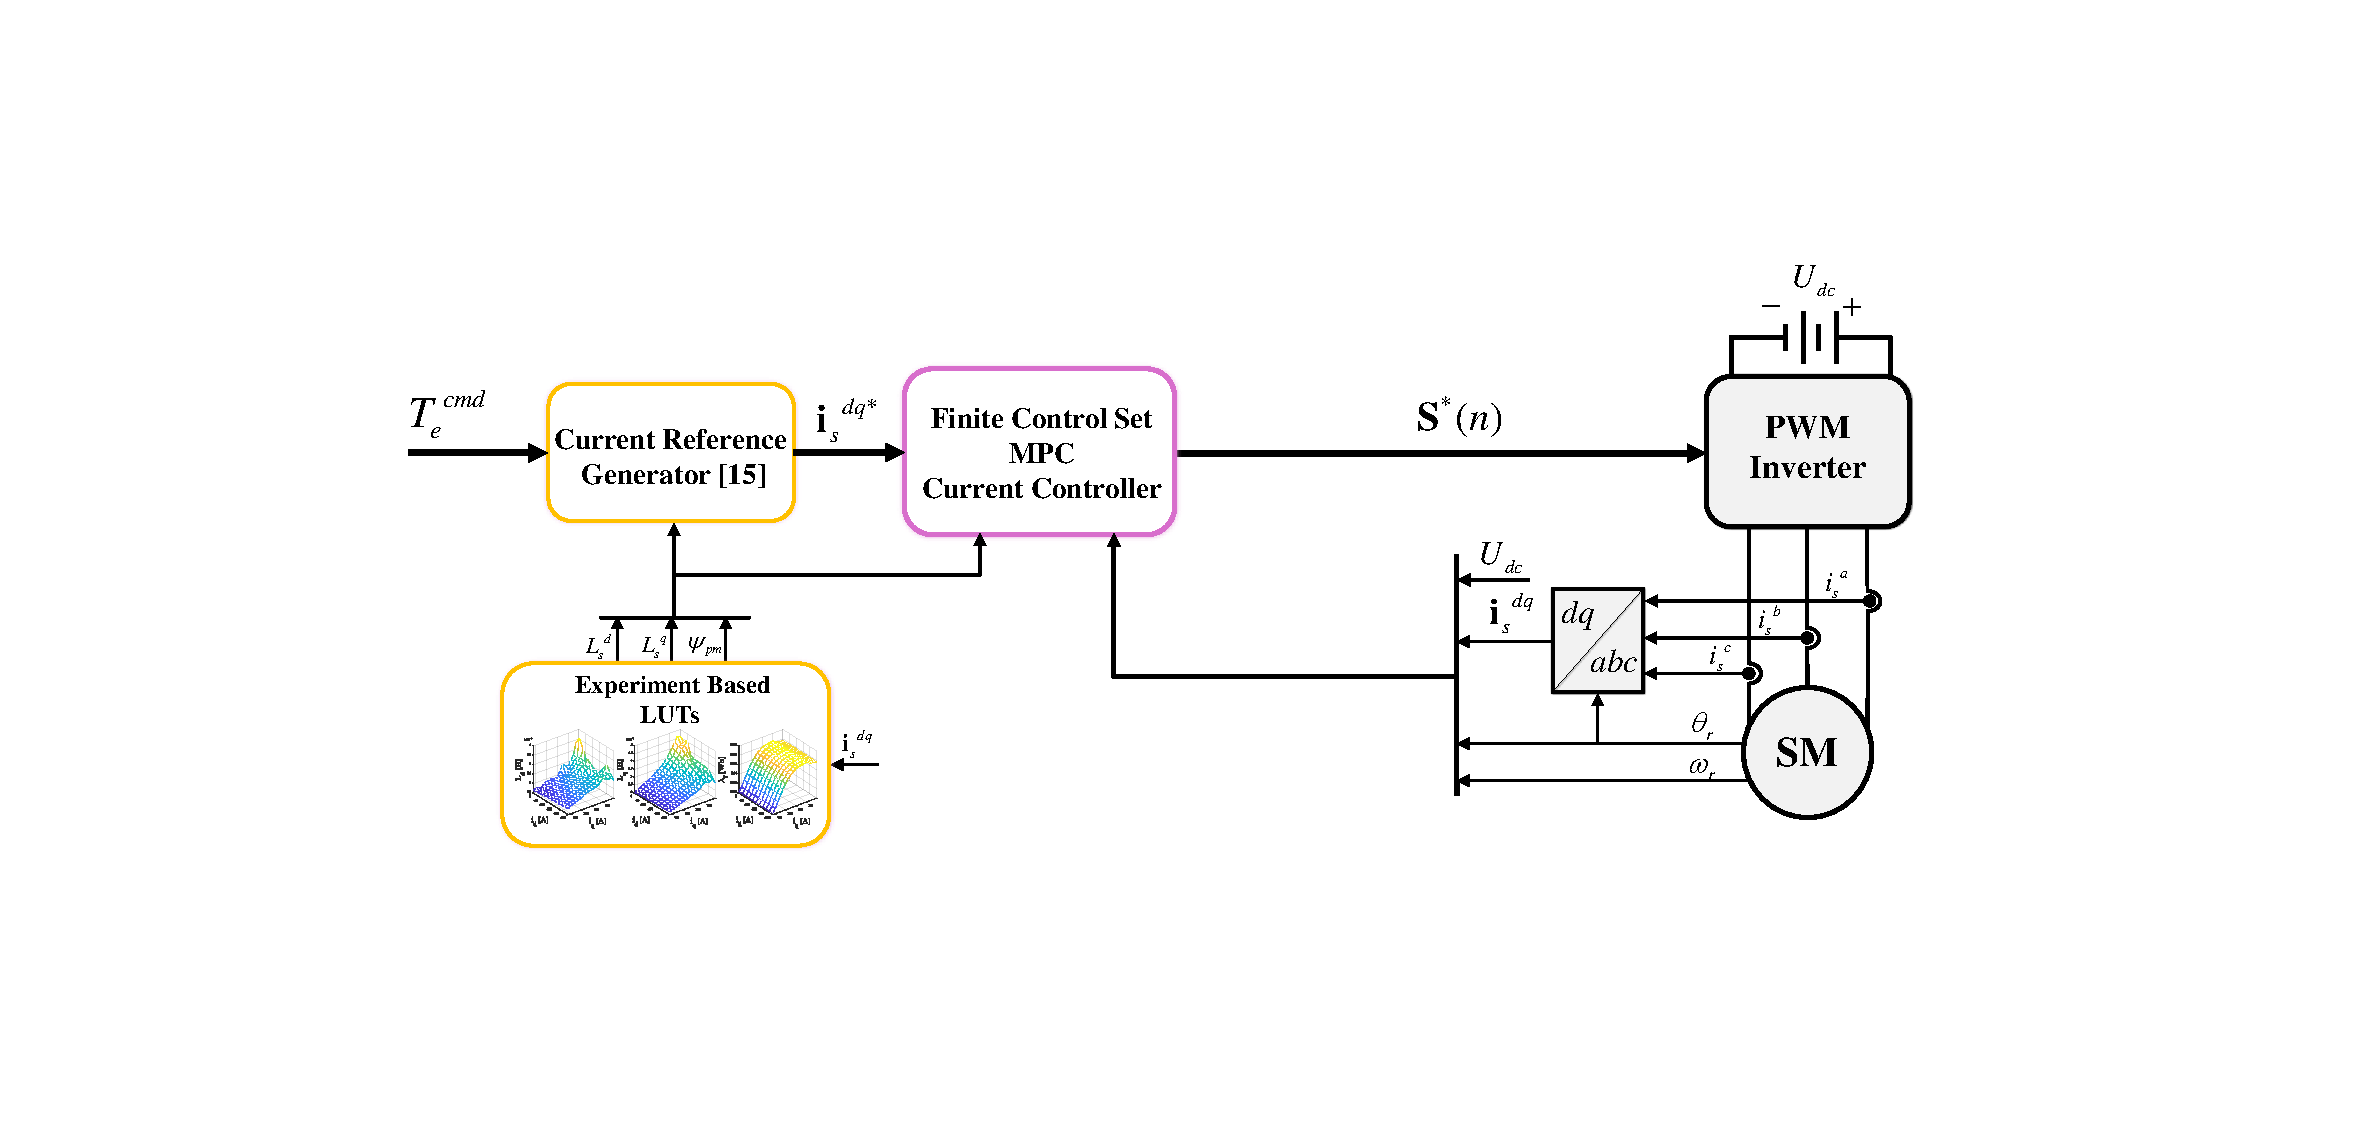
\includegraphics[scale=0.6]{chapters/Fig2.6.pdf}
    \caption{Control scheme using FCS-MPC current controller.}
    \label{Fig:2.6}
\end{figure}
\begin{algorithm}[!]
\caption{Predictive current control algorithm}
\begin{algorithmic}[1]
\STATE \textbf{Startup}
\STATE Measure $i_{dq}(k)$ and $\omega_r(k)$
\STATE $n = 0$
\FOR{$n \leq 7$}
\STATE $n = n + 1$
\STATE Calculate $\mathbf{u}^*_{dq}(k) \leftarrow {u_{s}^a}^*(n),{u_{s}^b}^*(n),{u_{s}^c}^*(n)$ using (\ref{eqn:2.18})$-$(\ref{eqn:2.20})
\STATE Predict $\mathbf{i}_{dq}(k+1)$ using (\ref{eqn:2.16}) and (\ref{eqn:2.17})
\STATE Evaluate cost function $g = |i_{d}^* - i_{d}^p| + |i_{q}^* - i_{q}^p|$
\STATE Store optimal values for $g$
\ENDFOR
\IF{$n = 7$}
    \STATE Apply the optimal space voltage vector $\mathbf{u}^*_n$ for minimum $g$
\ENDIF
\RETURN $\mathbf{u}^*_{dq}(k)$
\STATE Wait for next sampling instant
\end{algorithmic}\label{Algorithm:2.1}
\end{algorithm}
\begin{equation}\label{eqn:2.24}
g = \left| i_{d}^* - i_{d}^p \right| + \left| i_{q}^* - i_{q}^p \right|
\end{equation}

The accuracy of the predicted currents through FCS-MPCC is highly influenced by the machine parameters (inductance, stator, and permanent magnet flux linkages) \cite{c2.2_4}. However, as previously mentioned, machine parameters are not only nonlinear functions of stator currents but also very sensitive to temperature changes in the stator and rotor cores, as well as the stator windings and permanent magnets. Therefore, for robust control of FCS-MPCC, it is essential to develop a flux estimator or parameter identifier that can estimate and update the mismatched parameters in the prediction model online, thereby improving the accuracy of the predicted model.

\section{Existing Flux Linkage Estimators}\label{chap2:2.3} 
As mentioned above, online information on the machine parameters is essential not only for improving the operating performance of SMs (such as SM fault diagnosis, MTPA, etc.) but also for achieving robust optimal control of the predictive model, especially the FCS-MPCC method. However, it is extremely challenging to directly estimate all machine parameters using only the two current dynamics in (\ref{eqn:2.12}) and (\ref{eqn:2.13}) due to rank deficiency in the model equations (to estimate more than three parameters with only two equations) \cite{c2.3_3}. Therefore, instead of directly estimating the machine parameters, the stator flux linkage is first estimated \cite{c1_1},\cite{c2.3_4},\cite{c2.3_5},\cite{c2.3_6}, and then machine parameter identification is conducted online \cite{c2.3_1} or offline \cite{c2.3_2}. This section introduces existing methods for stator flux linkage estimation as a preliminary step for machine parameters estimation.

\subsection{Steady-State Assumption-based Flux Linkage Estimator} \label{sec2:2.3.1}
The machine dynamic model in (\ref{eqn:2.9}) can be rearranged as a flux-based dynamic model
\begin{align}\label{eqn:2.25}
\frac{d}{dt} \bm{\psi}^{dq}_s(t) = \mathbf{u}^{dq}_s(t) - R_s \mathbf{i}^{dq}_s(t) - \omega_r(t) \mathbf{J} \bm{\psi}^{dq}_s(t),
\end{align}
where the $d$-$q$ axis flux linkage vectors are constant in steady state, making the time derivative of the flux vector zero. Therefore, based on the steady-state assumption, the flux estimate vector can be simplified as
\begin{align}\label{eqn:2.26}
\bm{\hat \psi}^{dq}_s(s) = \frac{1}{\omega_r} \mathbf{J}^{-1} \left( \mathbf{u}^{dq*}_{s}(s) - \hat{R}_s \mathbf{i}^{dq}_s(s) \right),
\end{align}
where \(\hat{R}_s\) is the estimated stator resistance, which is a nonlinear function of the stator winding temperature but is assumed to be accurately estimable, and \(\bm{\hat{\psi}}^{dq}_s\) represents the estimate of the flux linkage vector. The electrical angular velocity \(\omega_r\) can be assumed to be constant because it is sufficiently slow compared to the electrical signals. The control input voltages \( u^{dq*}_{s} \) obtained from FCS-MPCC in (\ref{eqn:2.22}) and (\ref{eqn:2.23}) contain significant switching frequency components, so a low pass filter (LPF) is applied to filter out these high-frequency components, resulting in the flux estimate vector
\begin{align}\label{eqn:2.27}
\bm{\hat \psi}^{dq}_{s,\text{LPF}}(s) = \frac{\omega_\text{LPF}}{s + \omega_\text{LPF}} \bm{\hat \psi}^{dq}_s(s),
\end{align}
where \( \omega_\text{LPF} \) is the LPF cutoff frequency. 

This approach allows for the easy derivation of \(d\)- and \(q\)-axis flux estimates based on the steady state, so it is commonly used in many industries to obtain the parameters needed to create experiment-based lookup tables (LUTs). However, during transient states, this method produces significant estimation errors resembling spikes, distorts the magnitude and phase due to the cut-off frequency of the LPF, and is especially unsuitable for low-speed regions \cite{c2.3_7}, \cite{c2.3_8}, making it inappropriate for online estimation.

\subsection{Voltage and Current Model-based Flux Linkage Estimator} \label{sec2:2.3.2}
\subsubsection{Voltage Model}
The machine dynamic model in (\ref{eqn:2.5}) can be rearranged as a flux-based dynamic model
\begin{align}\label{eqn:2.28}
\frac{d}{dt}\bm{\psi}^{\alpha\beta}_s(t) = \mathbf{u}^{\alpha\beta}_s(t) - R_s \mathbf{i}^{\alpha\beta}_s(t),
\end{align}
which is defined as the \emph{voltage model} \cite{c2.1_1} for the flux linkage estimation. By purely integrating the voltage model in (\ref{eqn:2.28}), the flux estimate vector can be derived as follows 
\begin{align}\label{eqn:2.29}
\bm{\psi}^{\alpha\beta}_{s,\text{int}}(t) = \int_{0}^{t} \left( \bm{u}^{\alpha\beta*}_{s}(\tau) - \hat R_s \bm{i}^{\alpha\beta}_s(\tau) \right) d\tau + \bm{\psi}^{\alpha\beta}_{s,\text{int}}(0),
\end{align}
where \(\bm{{\psi}}^{\alpha\beta}_{s,{\text{int}}}:=({\psi}^{\alpha}_{s,{\text{int}}},{\psi}^{\beta}_{s,{\text{int}}})^\top\) is the integration result of the voltage model and \(\bm{{\psi}}^{\alpha\beta}_{s,{\text{int}}}(0):=({\psi}^{\alpha}_{s,{\text{int}}}(0),{\psi}^{\beta}_{s,{\text{int}}}(0))^\top\) is the flux estimate vector of the current model is the initial value of the flux vector. However, if there are errors in the input voltages $\bm{u}^{\alpha\beta*}_{s}$ and initial value $\bm{\psi}^{\alpha\beta}_{s,\text{int}}(0)$, or if sensor biases or inverter nonlinearities are present, the flux estimate obtained from simple integration will contain estimation errors (DC offset). 

To filter out the low-frequency DC offset components, a high-pass filter (HPF) is commonly applied to the flux estimate vector
\begin{align}\notag
\bm{\hat{\psi}}^{\alpha\beta}_{s,v}(s) &= \frac{s}{s + \omega_\text{HPF}} \times \frac{1}{s}\times\left[  \bm{u}^{\alpha\beta*}_{s}(s) - \hat{R}_s \bm{i}^{\alpha\beta}_{s}(s)\right]\\\label{eqn:2.37}
&= \frac{1}{s + \omega_\text{HPF}} \times \left[  \bm{u}^{\alpha\beta*}_{s}(s) - \hat{R}_s \bm{i}^{\alpha\beta}_s(s)\right]
\end{align}
in the S-domain \cite{c2.3_9}, \cite{c2.3_10}, where \(\bm{\hat{\psi}}^{\alpha\beta}_{s,{v}}:=(\hat{\psi}^{\alpha}_{s,{v}},\hat{\psi}^{\beta}_{s,{v}})^\top\) is the flux estimate vector of the voltage model and \(\omega_{\text{HPF}}\) is the cutoff frequency of the HPF.

While this approach performs well at high speeds (only in steady state), it becomes sensitive to filter gain settings near the cutoff frequency of the HPF, especially in low-speed regions, significantly distorting the magnitude and phase of the estimates.

\subsubsection{Current Model}
The flux linkage model in (\ref{eqn:2.10}) is defined as the \emph{current model} \cite{c2.1_1} and this flux vector is represented by the nominal inductance $\mathbf{{L}}^{dq}_{s,0}$ and permanent flux $\bm{{\psi}}^{dq}_{pm,0}$
\begin{align}\label{eqn:2.31}
\bm{\hat{\psi}}^{dq}_{s,i} &= \mathbf{{L}}^{dq}_{s,0}\mathbf{i}^{dq}_s
+ \bm\psi_{pm,0}, \quad 
 \mathbf{{L}}^{dq}_{s,0} = \begin{bmatrix}
{L}^d_{s,0} & 0 \\
0 & {L}^q_{s,0} \\
\end{bmatrix}, {\bm{{\psi}}^{dq}_{pm,0} = \begin{bmatrix}
{\psi_{pm,0}} \\
0
\end{bmatrix}},
\end{align}
where \(\bm{\hat{\psi}}^{dq}_{s,{i}}:=(\hat{\psi}^{q}_{s,{i}},\hat{\psi}^{q}_{s,{i}})^\top\) is the flux estimate vector of the current model in the ($d$,$q$)-reference frame.

This approach provides relatively robust flux estimation in low-speed and low-current regions. However, it cannot deal with the inaccuracies of machine parameters caused by magnetic saturation and temperature variations in permanent magnets, resulting in estimation errors.

\subsubsection{Hybrid Model}\begin{figure}[t]
    \centering
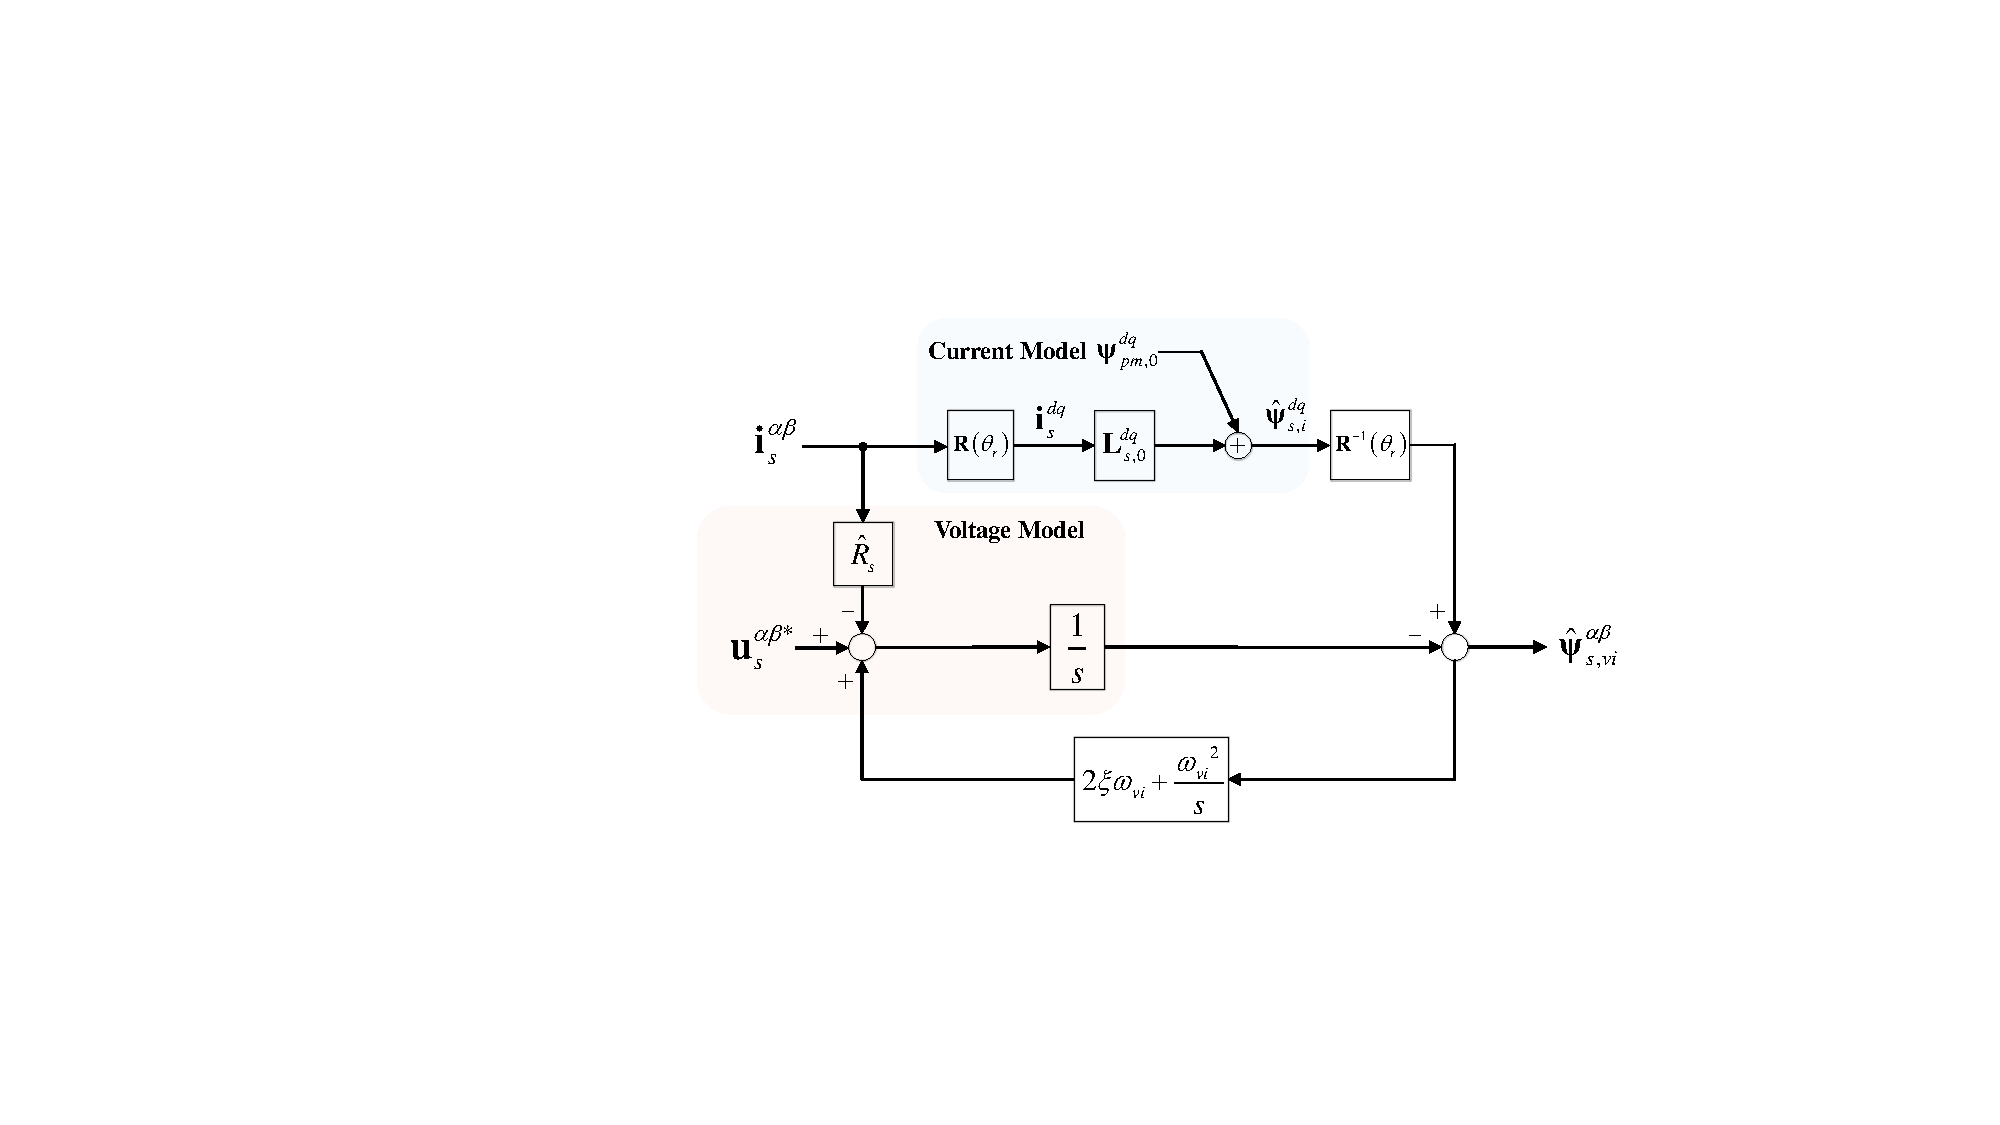
\includegraphics[scale=0.8]{chapters/Fig2.9.pdf}
    \caption{Block diagram of the voltage and current model-based flux linkage estimator.}
    \label{Fig:2.9}
\end{figure}
To overcome the disadvantages of the aforementioned voltage and current models, a Gopinath-style observer has been proposed, which uses the current model in low-speed regions and the voltage model in high-speed regions \cite{c2.3_11}, \cite{c2.3_12}, \cite{c2.3_13}, \cite{c2.3_14}. This observer uses a proportional-integral (PI) filter to smoothly transition between the flux estimates of the two models near the crossover frequency. The flux linkage estimate vector
\begin{align}\label{eqn:2.32}
\bm{\hat{\psi}}^{\alpha\beta}_{s,{vi}}(s)
=
\frac{s^2}{s^2 + 2 \xi \omega_{vi} s + \omega_{vi}^2}\bm{\hat{\psi}}^{\alpha\beta}_{s,v}(s) +
\frac{2 \xi \omega_{vi} s + \omega_{vi}^2}{s^2 + 2 \xi \omega_{vi} s + \omega_{vi}^2}\bm{R}^{-1}(\theta_r)\bm{\hat{\psi}}^{dq}_{s,i}(s)
\end{align}
in the ($\alpha$,$\beta$)-reference frame can be derived, where \(\bm{\hat{\psi}}^{\alpha\beta}_{s,{vi}}:=(\hat{\psi}^{\alpha}_{s,{vi}},\hat{\psi}^{\beta}_{s,{vi}})^\top\) represents the flux estimate vector of the voltage-current hybrid model, and \(\xi\) and \(\omega_{\text{vi}}\) denote the damping ratio and the natural frequency of the PI filter, respectively. Figure \ref{Fig:2.9} shows the block diagram of the flux observer based on the conventional voltage and current models.

Although this approach can be used to estimate flux linkages over a wide operating range, variations in the nominal parameters used in the current model can lead to a substantial decrease in estimation performance, especially during transient states. To address these drawbacks and ensure robustness against parameter variations, a modified flux observer for the voltage-current-based estimation model was presented in \cite{c2.3_15}, where the flux linkage errors caused by parameter inaccuracies can be determined by the output of the integral controller at steady state. 

However, this approach can significantly degrade estimation performance at low speeds because the reciprocal of the rotor speed affects the flux estimates. Additionally, there has been insufficient research on improving estimation performance during transient states, and there is a lack of information on selecting the cutoff frequency for the PI filter. Without precise criteria for filter design, phase, and magnitude distortions can occur in the estimates, significantly affecting estimation performance, especially during transient states. 

\subsection{Disturbance Observer-based Flux Linkage Estimator \cite{c1_1}}\label{chap2:2.3.3}
The novel approach of estimating nonlinear flux linkages in the time domain using a disturbance observer-based state observer was introduced in \cite{c1_1}. This estimator is very simple and highly effective for nonlinear flux linkage estimation. The key idea is to separate the $d$-$q$ axis flux linkage vector in (\ref{eqn:2.10}) into a linear term $\mathbf{L}_{s,0}\mathbf{i}^{dq}_{s}$ and a nonlinear flux linkage term $\Delta\boldsymbol{\psi}^{dq}_s(\mathbf{i}^{dq}_s)$, i.e.
\begin{align}\label{eqn:2.33}
\bm{\psi}^{dq}_s(t) = \mathbf{L}^{dq}_{s,0} \mathbf{i}^{dq}_s(t) + \underbrace{\left( \mathbf{L}^{dq}_{s} - \mathbf{L}^{dq}_{s,0} \right) \mathbf{i}^{dq}_s(t) + \boldsymbol{\psi}^{dq}_{pm}}_{=:\Delta{\boldsymbol{\psi}^{dq}_s}(\mathbf{i}^{dq}_s)=\Delta{\boldsymbol{\psi}^{dq}_s}(t)} \xLeftrightarrow{\hspace{0.5cm}} \ \mathbf{i}^{dq}_s(t) = {\mathbf{L}^{dq}_{s,0}}^{-1}\left(\bm{\psi}^{dq}_s(t) - \Delta{\boldsymbol{\psi}^{dq}_s}(t)\right)
\end{align}
with constant (but arbitrarily) nominal (static) inductance matrix $\mathbf{L}^{dq}_{s,0} \in \mathbb{R}^{2\times 2}$ and nonlinear flux vector $\Delta\boldsymbol{\psi}^{dq}_s:=(\Delta{\psi}^{d}_s,\Delta{\psi}^{q}_s)^\top$, including cross-coupling and saturation effects. 
The time derivative of the nonlinear flux linkage in (\ref{eqn:2.33})
\begin{align}\label{eqn:2.34}
\frac{d}{dt}\Delta{\boldsymbol{\psi}^{dq}_s} = \underbrace{\mathbf{\dot L}^{dq}_{s} \mathbf{i}^{dq}_s + \left( \mathbf{L}^{dq}_{s} - \mathbf{L}^{dq}_{s,0} \right) \mathbf{\dot i}^{dq}_s + \boldsymbol{\dot \psi}^{dq}_{pm}}_{=:\mathbf{d}^{dq}_s(\mathbf{i}^{dq}_s,\mathbf{\dot i}^{dq}_s) = \mathbf{d}^{dq}_s(t)}
\end{align}  
can be derived, where the lumped disturbance vector $\mathbf{d}^{dq}_s:=(d^{d}_s,d^{q}_s)^\top$ can be expressed as a nonlinear function of the current $\mathbf{i}^{dq}_s$ and the derivative of the current $\mathbf{\dot i}^{dq}_s$. Since it is very difficult to know the exact model for these disturbance signals, the physical behaviors of the dynamics in (\ref{eqn:2.34}) can be explained by the following assumption.

\textbf{Assumption (A.2.1)} The dynamics system in (\ref{eqn:2.9}) are bounded-input-bounded-output (BIBO) stable and the lumped disturbance vector in (\ref{eqn:2.34}) is upper bounded by
\begin{equation}\notag
   ||\mathbf{d}^{dq}_s|| \stackrel{(\ref{eqn:2.34})}\leq  ||\mathbf{\dot L}^{dq}_{s}|| ||\mathbf{i}^{dq}_s|| +  ||\mathbf{L}^{dq}_{s} - \mathbf{L}^{dq}_{s,0}||  ||\mathbf{\dot i}^{dq}_s|| + ||\boldsymbol{\dot \psi}^{dq}_{pm}||.
\end{equation}
\textbf{Assumption (A.2.2)}
All parameters and signals in the ($d$,$q$)-reference frame in (\ref{eqn:2.33}) become constant in steady state (i.e. constant current and speed), so the nonlinear flux linkage $\Delta\boldsymbol{\psi}^{dq}_s$ has the characteristics
\begin{equation}\notag
    \Delta\boldsymbol{\psi}^{dq}_s(t) = \left( \mathbf{L}^{dq}_{s} - \mathbf{L}^{dq}_{s,0} \right) \mathbf{i}^{dq}_s(t) + \boldsymbol{\psi}^{dq}_{pm} = \mathbf{c}^{dq}_s,
\end{equation}
with unknown but constant $\mathbf{c}^{dq}_s:=(c^{d}_s,c^{q}_s)^\top$ and their time derivatives become zero vector (only) in steady state. Therefore, the disturbance vector $\mathbf{d}^{dq}_s $ in (\ref{eqn:2.34}) becomes the zero vector \(\mathbf{O}_2\), i.e. 
\begin{align}\notag
    \mathbf{d}^{dq}_s \rightarrow \mathbf{O}_2 \quad \left(
    \mathbf{\dot L}^{dq}_{s}\rightarrow \mathbf{O}_{2\times2}, \mathbf{\dot i}^{dq}_s \rightarrow \mathbf{O}_2, \boldsymbol{\dot \psi}^{dq}_{pm} \rightarrow \mathbf{O}_2 \text{ as } t \rightarrow \infty 
    \right)
\end{align}
which means that these disturbance signals can be assumed to be step signals.

Substituting (\ref{eqn:2.33}) into (\ref{eqn:2.9}) leads to the altered dynamic model
\begin{equation}
\begin{aligned}\label{eqn:2.35}
\begin{cases}
\frac{d}{dt}{\bm{\psi}}^{dq}_s(t) = \mathbf{u}^{dq}_s(t) - R_s {\mathbf{L}^{dq}_{s,0}}^{-1} \left( \bm{\psi}^{dq}_s(t) - \Delta{\boldsymbol{\psi}^{dq}_s}(t) \right) - \omega_r(t) \mathbf{J} \bm{\psi}^{dq}_s(t) \\
\frac{d}{dt}{\Delta}{\boldsymbol{\psi}^{dq}_s}(t) = \mathbf{d}^{dq}_s(t) \\
\mathbf{i}_{dq}(t) = {\mathbf{L}^{dq}_{s,0}}^{-1} \left( \bm{\psi}^{dq}_s(t) - \Delta{\boldsymbol{\psi}^{dq}_s}(t) \right)
\end{cases}
\end{aligned}.
\end{equation}
By defining the nonlinear flux linkage vector $\Delta{\boldsymbol{\psi}^{dq}_s}$ as an extended state to be estimated, the state-space model is expressed as
\begin{equation}\label{eqn:2.36}
\left\{
\begin{aligned}
\frac{d}{dt}\mathbf{x}(t) &= \mathbf{A}(\omega_r)\mathbf{x}(t) + \mathbf{B}\mathbf{u}(t) + \mathbf{d}(t) \\
\mathbf{y}(t) &= \mathbf{C}\mathbf{x}(t)
\end{aligned}
\right.
\end{equation}
with 
\begin{equation*}
\begin{aligned}
\mathbf{x} &:= \begin{pmatrix} \bm{\psi}^{dq}_s \\ \Delta{\boldsymbol{\psi}^{dq}_s} \end{pmatrix}, \quad \mathbf{u} := \mathbf{u}^{dq}_s, \quad \mathbf{y} := \mathbf{i}^{dq}_s, \quad \mathbf{O}_{2\times2} := \begin{bmatrix}
0  & 0\\
0 & 0
\end{bmatrix}, \quad \mathbf{I}_{2\times2} := \begin{bmatrix}
1  & 0\\
0 & 1
\end{bmatrix}, \\
\mathbf{A}(\omega_r) &:= \begin{bmatrix}
-R_s {\mathbf{L}^{dq}_{s,0}}^{-1}-\omega_r \mathbf{J}  & R_s {\mathbf{L}^{dq}_{s,0}}^{-1}\\
\mathbf{O}_{2\times2} & \mathbf{O}_{2\times2}
\end{bmatrix}, \quad \mathbf{B} := \begin{bmatrix}
\mathbf{I}_{2\times2} \\
\mathbf{O}_{2\times2}
\end{bmatrix}, \quad \mathbf{C} := \begin{bmatrix}
{\mathbf{L}^{dq}_{s,0}}^{-1} & -{\mathbf{L}^{dq}_{s,0}}^{-1}
\end{bmatrix}, \\
\mathbf{d} &:= \begin{bmatrix}
    \mathbf{O}_2 & \mathbf{d}^{dq}_s
\end{bmatrix}^\top, \quad \mathbf{O}_2 := \begin{bmatrix}
    0 & 0
\end{bmatrix}^\top,
\end{aligned}
\end{equation*}
where $\mathbf{x}$ represents the state vector, $\mathbf{u}$ denotes the input vector, $\mathbf{y}$ represents the output vector and $\mathbf{d}$ is the lumped disturbance vector. The matrix $\mathbf{A}(\omega_r)$ is the system matrix with respect to $\omega_r$, $\mathbf{B}$ is the input matrix, and $\mathbf{C}$ is the output matrix. 

To verify if the dynamic system in (\ref{eqn:2.36}) is in an observable form for constant speed $\omega_r$, the observability matrix 
\begin{equation}\label{eqn:2.37}
\mathbf{\mathcal{O}}(\omega_r) = \begin{bmatrix}
\mathbf{C} \\
\mathbf{CA}(\omega_r) \\
\mathbf{CA}(\omega_r)^2 \\
\mathbf{CA}(\omega_r)^3
\end{bmatrix}
\end{equation}
needs to be examined; since the matrix in (\ref{eqn:2.37}) has full rank (i.e., $\mathbf{\mathcal{O}}(\omega_r) = 4$), all states $\mathbf{x}$ can be observed. Accordingly, a linear observer can be designed as follows
\begin{equation}\label{eqn:2.38}
\left\{
\begin{aligned}
\frac{d }{dt}\hat{\mathbf{x}}(t) &= \left[ \mathbf{A}(\omega_r) - \mathbf{F}(\omega_r) \mathbf{C} \right] \hat{\mathbf{x}}(t) + \mathbf{B} \mathbf{u}(t) + \mathbf{F}(\omega_r) \mathbf{y}(t) \\
\hat{\mathbf{y}}(t) &= \mathbf{C} \hat{\mathbf{x}}(t)
\end{aligned},
\right.
\end{equation}
where $\hat{\mathbf{x}}$ and $\hat{\mathbf{y}}$ represent the estimated vector of $\mathbf{x}$ and $\mathbf{y}$, respectively, and $\mathbf{F}(\omega_r) \in \mathbb{R}^{4 \times 2}$ denotes the gain matrix of the observer and depends on the electrical angular speed. To analyze the stability of the estimation convergence, subtracting (\ref{eqn:2.38}) from (\ref{eqn:2.36}) leads to the estimation error dynamics
\begin{equation}\label{eqn:2.39}
\frac{d}{dt}\mathbf{e}(t) = \left[\mathbf{A}(\omega_r) - \mathbf{F}(\omega_r)\mathbf{C}\right] \mathbf{x}(t) - \mathbf{d}(t)
\end{equation}
with the estimation error
\begin{equation}\notag
\mathbf{\tilde x}(t) :=\mathbf{\hat x}(t) - \mathbf{x}(t),
\end{equation}
where \(\mathbf{d} \rightarrow 0\) as \( t \rightarrow \infty \), recalling Assumption (A.2.1) and Assumption (A.2.2). If the gain matrix \(\mathbf{F}(\omega_r)\) is designed such that \(\mathbf{A}-\mathbf{F}(\omega_r)\mathbf{C}\) becomes a stable Hurwitz matrix (i.e., with the desired eigenvalues or poles within the negative complex half-plane), the estimation error \(\mathbf{\tilde{x}}\) will decay exponentially and asymptotically to the equilibrium point. Figure \ref{Fig:2.10} shows the observer block diagrams for DOB-FLE. 
\begin{figure}[t]
    \centering   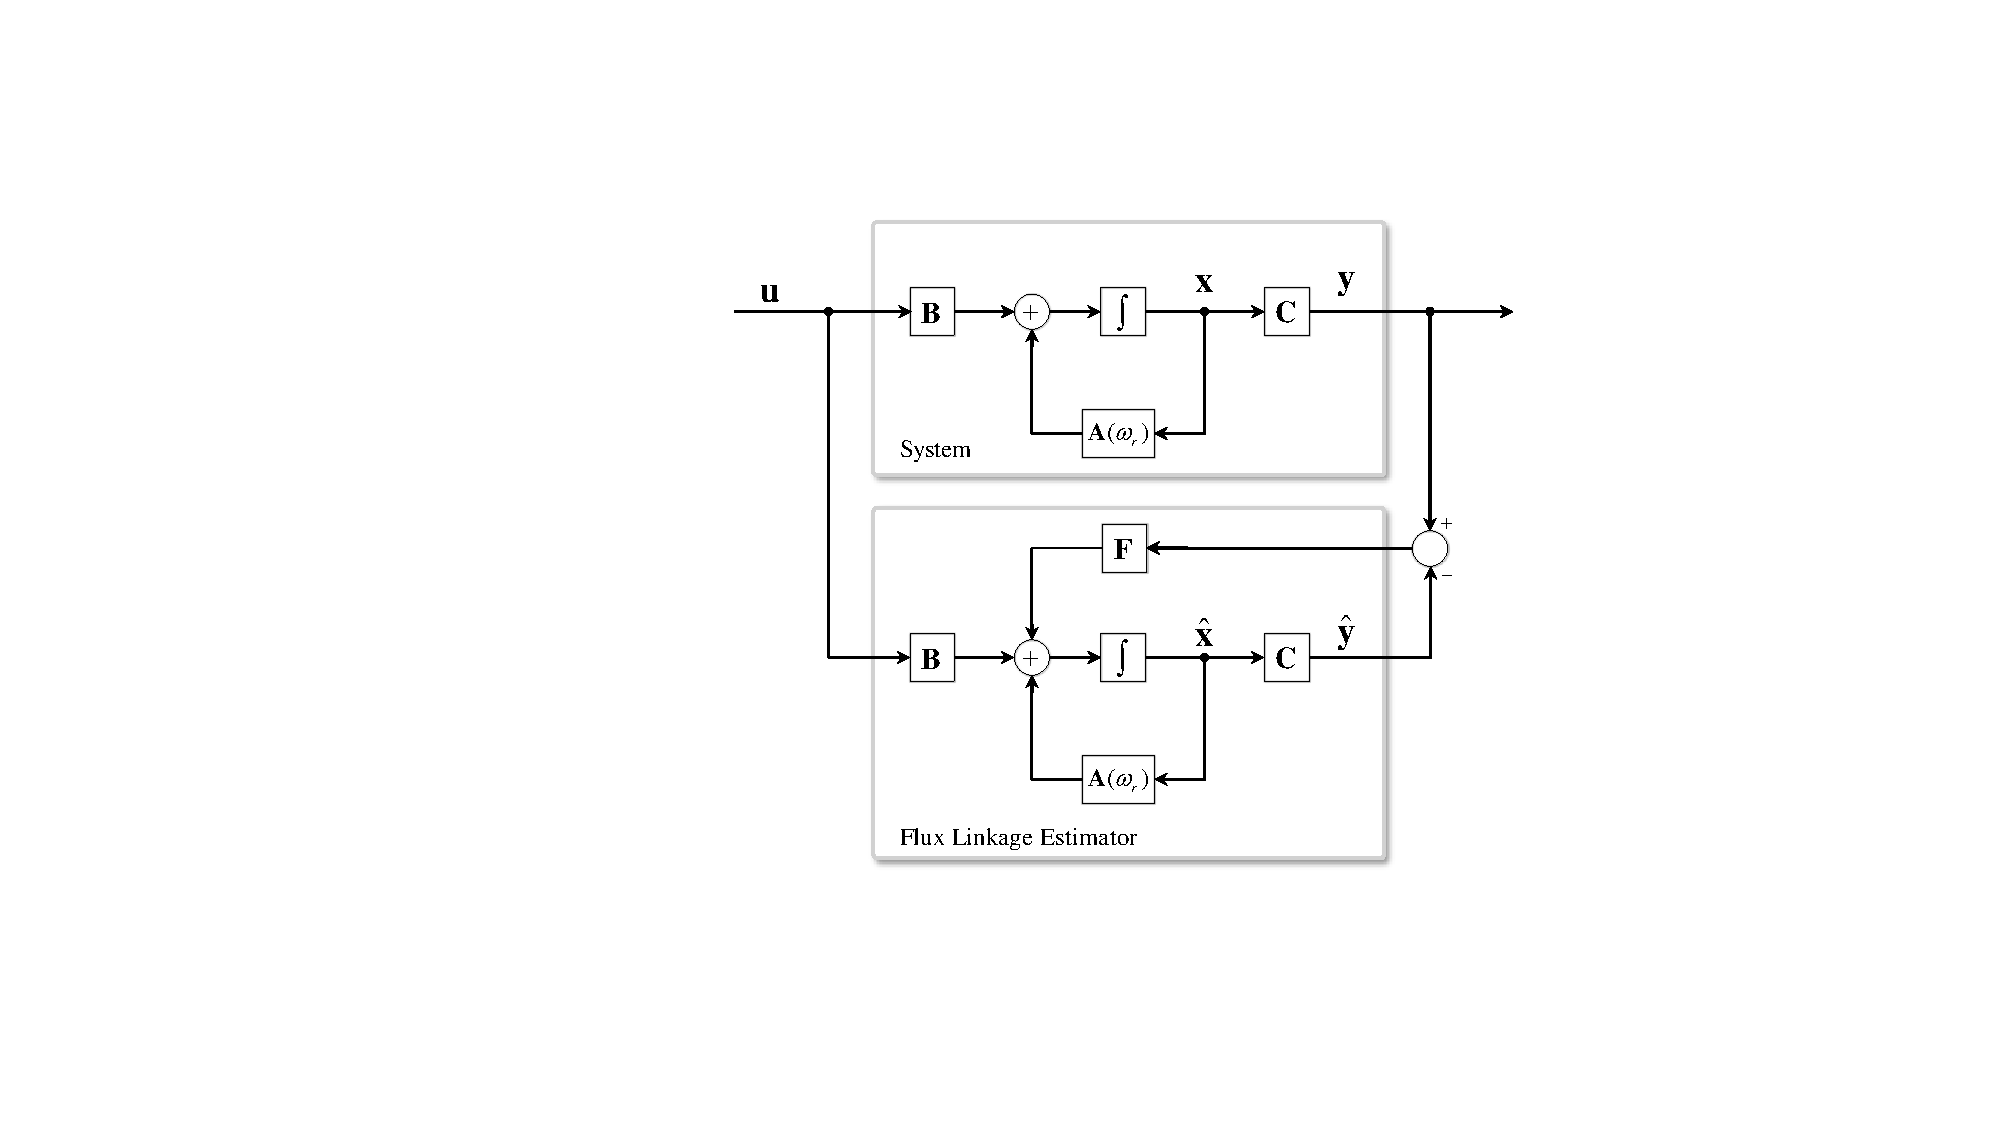
\includegraphics[scale=0.7]{chapters/Fig3.1.pdf}
    \caption{Observer block diagram for DOB-FLE.}
    \label{Fig:2.10}
\end{figure}

DOB-FLE separates the stator flux linkage vector \(\boldsymbol{\psi}^{dq}_s\) into a linear flux with nominal inductance \(\mathbf{L}^{dq}_{s,0}\) and the remaining nonlinear flux term \(\Delta\boldsymbol{\psi}^{dq}_s\), assuming this nonlinear flux term as a constant disturbance signal (i.e. step signal). Therefore, this approach allows for exponential estimation of the nonlinear flux term through a simple linear observer. However, in transient states where the current ramps up or down, the disturbance signals are time-varying with a certain slope rather than constant, causing the magnitude of the disturbance \(\mathbf{d}\) in (\ref{eqn:2.36}) to increase. Additionally, if an inaccurate nominal inductance is used in the observer, the norm of the disturbance vector \(\|\mathbf{d}\|\) increases, leading to significant transient estimation errors.




\end{spacing}

%%%%%%%%%%%%%%%%%%%%%%%%%%%%%%%%%%%%
% Chapter 3
%%%%%%%%%%%%%%%%%%%%%%%%%%%%%%%%%%%%

\begin{spacing}{2.0}

\chapter{Proposed Methods for Online Stator Flux Linkage Estimation}\label{chapter3}
Since the measurements available from the SMs outputs are limited to stator current, electrical angular velocity, and position, it is not possible to directly estimate the flux linkage using a state observer designed based on the flux dynamics models in (\ref{eqn:2.9}) and (\ref{eqn:2.28}) (unobservable model). Section \ref{sec2:2.3.2} introduced a flux estimation method using a PI filter-based hybrid model to remove DC offsets occurring from purely integrating the stator flux linkage dynamics in (\ref{eqn:2.28}). However, the cutoff frequency of the filters degrades the transient estimation performance. Specifically, in control methods like FCS-MPC, using filters causes magnitude and phase distortions of the estimates due to filtered specific frequencies in the voltage input \cite{c3.2_1}. Section \ref{chap2:2.3.3} presented a method to estimate flux linkage by separating it into a linear flux term with nominal inductance and the remaining nonlinear flux term, extending this as an extended disturbance state to make it observable, and designing a state observer in the time domain. However, the flux estimation performance depends on the accuracy of the nominal parameter, and if it is inaccurate, the transient estimation performance may deteriorate.

In this chapter, two flux linkage estimators that can improve the estimation performance of existing flux estimators are proposed: the Extended State Observer-based Flux Linkage Estimator (ESO-FLE) and the Integration Error and Parameter Update-Based Flux Linkage Estimator (IE-PU-FLE). The main contributions of these estimators are (i) the development of an observable model based on the stator flux linkage dynamics, (ii) the design of the state observer in the time domain to prevent magnitude and phase distortion of the estimates caused by filters (i.e. LPF and HPF), especially in FCS-MPC switching method, and (iii) the reduction of dependence on nominal parameters used in the estimators, thereby improving transient estimation performance.

\section{Extended State Observer-based Flux Linkage Estimator \cite{c3.1_1}}\label{chap3:3.1}
The DOB-FLE in Section \ref{chap2:2.3.3} defines the nonlinear flux \(\Delta\boldsymbol{\psi}^{dq}_s\) as a disturbance step signal based on assumptions (A.2.1) and (A.2.2), and extends it as an additional state to be estimated. However, while this approach exhibits excellent estimation performance in steady state, its transient estimation performance is determined by the accuracy of the nominal inductance parameter ${\mathbf{L}^{dq}_{s,0}}$ used in the estimator. It means that the transient estimation performance depends on the parameter accuracy, and if the parameters are inaccurate, the nonlinear flux linkage \(\Delta\boldsymbol{\psi}^{dq}_s\) may be time-varying with a constant slope in transient state. In this section, to improve the transient estimation performance of the DOB-FLE, an extended state observer-based flux linkage estimator (ESO-FLE) is proposed. The key idea is to define the nonlinear flux \(\Delta\boldsymbol{\psi}^{dq}_s\) as a ramp signal with a constant slope and estimate it by extending this constant slope as an additional state to be estimated. 

The nonlinear flux linkage \(\Delta\boldsymbol{\psi}^{dq}_s\) (i.e. step disturbance signal) in Assumption (A.2.1) can be assumed as ramp disturbance signals
\begin{equation}\label{eqn:3.1}
\begin{aligned}
    \Delta\boldsymbol{\psi}^{dq}_s(t) = \left( \mathbf{L}^{dq}_{s} - \mathbf{L}^{dq}_{s,0} \right) \mathbf{i}^{dq}_s(t) + \boldsymbol{\psi}^{dq}_{pm} = \mathbf{c}^{dq}_s + \mathbf{l}^{dq}_s t,
\end{aligned}
\end{equation}
with unknown but constant slope \(\mathbf{l}^{dq}_s := (l^d_s,\ l^q_s)^\top\), which is extended the additional state to be estimated. The time derivative of the nonlinear flux linkage in (\ref{eqn:3.1}) can be expressed as 
\begin{align}\label{eqn:3.2}
\frac{d}{dt}\Delta{\boldsymbol{\psi}^{dq}_s} = \underbrace{\mathbf{\dot L}^{dq}_{s} \mathbf{i}^{dq}_s + \left( \mathbf{L}^{dq}_{s} - \mathbf{L}^{dq}_{s,0} \right) \mathbf{\dot i}^{dq}_s + \boldsymbol{\dot \psi}^{dq}_{pm}}_{\stackrel{(\ref{eqn:2.34})}= \mathbf{d}^{dq}_s(t)} = \mathbf{l}^{dq}_s(t),
\end{align}  
where, the time derivative of the constant slope $\mathbf{l}^{dq}_s$ in (\ref{eqn:3.2}) is represented as 
\begin{align}\label{eqn:3.3}
\frac{d}{dt}{\mathbf{l}^{dq}_s} = \underbrace{\mathbf{\ddot L}^{dq}_{s}\mathbf{i}^{dq}_s+2\mathbf{\dot L}^{dq}_{s} \dot{\mathbf{i}}^{dq}_s + \left( \mathbf{L}^{dq}_{s} - \mathbf{L}^{dq}_{s,0} \right) \mathbf{\ddot i}^{dq}_s + \boldsymbol{\ddot \psi}^{dq}_{pm}}_{=:  \mathbf{d}^{dq,l}_s(t) \rightarrow  0 \text{ as t} \rightarrow \infty},
\end{align}  
with the lumped disturbance vector $\mathbf{d}^{dq,l}_s:=(d^{d,l}_s,d^{q,l}_s)^\top$. Recalling Assumption (A.2.1), the lumped disturbance vector \(\mathbf{d}^{dq,l}_s\) can be upper bounded (all parameters and signals become constant in steady state) and becomes zero in steady state. Accordingly, the altered dynamic model is summarized as follows
\begin{equation}
\begin{aligned}\label{eqn:3.4_1}
\begin{cases}
\frac{d}{dt}{\bm{\psi}}^{dq}_s(t) = \mathbf{u}^{dq}_s(t) - R_s {\mathbf{L}^{dq}_{s,0}}^{-1} \left( \bm{\psi}^{dq}_s(t) - \Delta{\boldsymbol{\psi}^{dq}_s}(t) \right) - \omega_r(t) \mathbf{J} \bm{\psi}^{dq}_s(t) \\
\frac{d}{dt}{\Delta}{\boldsymbol{\psi}^{dq}_s}(t) = \mathbf{l}^{dq}_s(t) \\
\frac{d}{dt}{\boldsymbol{l}^{dq}_s}(t) = \mathbf{d}^{dq,l}_s(t) \\
\mathbf{i}_{dq}(t) = {\mathbf{L}^{dq}_{s,0}}^{-1} \left( \bm{\psi}^{dq}_s(t) - \Delta{\boldsymbol{\psi}^{dq}_s}(t) \right)
\end{cases}
\end{aligned}.
\end{equation}
Based on the dynamics in (\ref{eqn:3.4_1}), the state-space model 
\begin{align}\label{eqn:3.5_1}
&\left\{
\begin{aligned}
    \frac{d}{dt}{\mathbf{x}}(t) &= \mathbf{A}(\omega_r)\mathbf{x}(t) + \mathbf{B}\mathbf{u}(t) + \mathbf{d}(t)\\
    \mathbf{y}(t) &= \mathbf{C}\mathbf{x}(t)
\end{aligned}
\right.
\end{align}
with
\begin{equation*}
\begin{aligned}
\mathbf{x} &:= 
\begin{pmatrix}
\boldsymbol{\psi}^{dq}_s \\ \Delta\boldsymbol{\psi}^{dq}_s \\ \mathbf{l}^{dq}_s
\end{pmatrix}, \quad \mathbf{u} := \mathbf{u}^{dq}_s, \quad \mathbf{y} := \mathbf{i}^{dq}_s, \quad \mathbf{O}_{2\times2} := \begin{bmatrix}
0  & 0\\
0 & 0
\end{bmatrix}, \quad \mathbf{I}_{2\times2} := \begin{bmatrix}
1  & 0\\
0 & 1
\end{bmatrix}, \\
\mathbf{A}(\omega_r) &:= 
\begin{bmatrix}
-R_s {\mathbf{L}^{dq}_{s,0}}^{-1} - \omega_r \mathbf{J} & R_s {\mathbf{L}^{dq}_{s,0}}^{-1} & \mathbf{O}_{2\times2} \\
\mathbf{O}_{2\times2} & \mathbf{O}_{2\times2} & \mathbf{I}_{2\times2} \\
\mathbf{O}_{2\times2} & \mathbf{O}_{2\times2} & \mathbf{O}_{2\times2}
\end{bmatrix}, \mathbf{B} := \begin{bmatrix}
\mathbf{I}_{2\times2} \\
\mathbf{O}_{2\times2} \\
\mathbf{O}_{2\times2}
\end{bmatrix}, \mathbf{C} := 
\begin{bmatrix}
{\mathbf{L}^{dq}_{s,0}}^{-1} \\ -{\mathbf{L}^{dq}_{s,0}}^{-1} \\ \mathbf{O}_{2\times2}
\end{bmatrix}^\top, \\
\mathbf{d} &:= \begin{bmatrix}
    \mathbf{O}_2 & \mathbf{O}_2 & \mathbf{d}^{dq,l}_s
\end{bmatrix}^\top, \quad \mathbf{O}_2 := \begin{bmatrix}
    0 & 0
\end{bmatrix}^\top,
\end{aligned}
\end{equation*}
where $\mathbf{x}$ represents the state vector, $\mathbf{u}$ denotes the input vector, $\mathbf{y}$ represents the output vector and $\mathbf{d}$ is the lumped disturbance vector. The matrix $\mathbf{A}(\omega_r)$ is the system matrix with respect to $\omega_r$, $\mathbf{B}$ is the input matrix, and $\mathbf{C}$ is the output matrix. 

To analyze whether the states of the dynamic system in (\ref{eqn:3.4_1}) are fully observable, the observability matrix is analyzed (for constant $\omega_r$), i.e.
\begin{equation}\label{eqn:3.6_1}
\mathbf{\mathcal{O}}(\omega_r) = \begin{bmatrix}
\mathbf{C} \\
\mathbf{CA}(\omega_r) \\
\vdots \\
\mathbf{CA}(\omega_r)^5
\end{bmatrix},
\end{equation}
which is evaluated using the first three rows of $\mathbf{\mathcal{O}}(\omega_r)$ for simplicity. Consequently, the observability matrix has a full rank (i.e., $\mathbf{\mathcal{O}}(\omega_r) = 6$) if $\omega_r \neq 0$, and the state $\mathbf{x}$ is (locally) fully observable. The method for designing an observer for flux estimation is the same as that mentioned in DOB-FLE.

ESO-FLE assumes the nonlinear flux as a time-varying ramp disturbance signal with a constant slope and extends this slope as an additional state to be estimated. This approach improves transient estimation performance by considering the rapidly changing current behavior or additional disturbance signals caused by incorrect nominal inductance. However, if noise or uncertainties exist in the extended states, the estimates become highly sensitive to the observer's gain matrix, so it is crucial to select the optimal gain accordingly.

\section{Integration Error Estimation and Parameter Update-Based Flux Linkage Estimator} \label{sec3:3.2.1}
As above mentioned, purely integrating the voltage model in (\ref{eqn:2.28}) results in the actual flux linkage in the ($\alpha$,$\beta$)-reference frame and the integration errors caused by discrepancies. Therefore, this section presents (i) an observable model that can directly estimate these integration errors and proposes a state observer in the time domain that directly compensates for these integration errors from the integration results. Additionally, since the selection of the nominal inductance used in the observer determines the transient estimation performance, this section proposes (ii) a method to update this value to reflect the actual value, thereby improving transient estimation performance. Furthermore, (iii) an adaptive observer that is robust to parameter variations is suggested.

\subsection{Flux Linkage Estimation based on Integration Error Estimation}
\subsubsection{Flux Model Reformulation for Integration Error Estimation}
The pure integration results of the voltage model in (\ref{eqn:2.28}) can be physically separated into the actual flux linkage term $\boldsymbol{\psi}^{\alpha\beta}_s$ and the integration error term $\boldsymbol{O}^{\alpha\beta}_s$, which is accumulated due to input and initial value errors \cite{c3.2_1}, i.e.
\begin{align}\notag
\bm{\psi}^{\alpha\beta}_{s,\text{int}}(t) &= \int_{0}^{t} \left( \bm{u}^{\alpha\beta*}_{s}(\tau) - \hat R_s \bm{i}^{\alpha\beta}_s(\tau) \right) d\tau + \bm{\psi}^{\alpha\beta}_{s,\text{int}}(0)
\\\label{eqn:3.4}
&= \boldsymbol{\psi}^{\alpha\beta}_s(t) + \boldsymbol{O}^{\alpha\beta}_s(t) 
\end{align}
with $\boldsymbol{\psi}^{\alpha\beta}_s := (\psi^{\alpha}_s, \psi^{\beta}_s)^T$ and $\boldsymbol{O}^{\alpha\beta}_s := (O^{\alpha}_s, O^{\beta}_s)^T$. The $d$-$q$ axis flux linkages in (\ref{eqn:2.10}) can be rearranged by expressing them as
\begin{align}\notag
\boldsymbol\psi^{dq}_s(t) 
&= 
\mathbf{L}^{dq}_s(t)
\mathbf{i}^{dq}_s(t)
+
\boldsymbol{\psi}^{dq}_{pm}(t) \\
&= 
L^q_s(t)\boldsymbol{i}^{dq}_s(t)
+
\begin{bmatrix}
    \underbrace{(L^d_s(t) - L^q_s(t))i^d_s(t) + \psi_{pm}(t)}_{=:\Delta\psi^d_s(t)} \\
    0
\end{bmatrix}\label{eqn:3.5}
\end{align}
using only the $q$-axis inductance as a proportional constant, where $\Delta\psi^d_s$ denotes the $d$-axis nonlinear flux linkage caused by the saliency of the SMs rotor and the permanent magnetic flux linkage. 

By applying the inverse of the simplified Park transformation in (\ref{eqn:2.8}) to (\ref{eqn:3.5}), the stator flux linkage vector in the ($\alpha$,$\beta$)-reference frame can be obtained as follows
\begin{align}\label{eqn:3.6a}
\boldsymbol{\psi}^{\alpha\beta}_s(t) &= L^q_s(t) \mathbf{i}^{\alpha\beta}_s(t) + 
\mathbf{P}(\theta_r)
\Delta \psi^{d}_s(t)\\\label{eqn:3.6b}
&= \hat{L}^q_s(t) \mathbf{i}^{\alpha\beta}_s(t) + 
 \underbrace{(L^q_s(t) -\hat{L}^q_s(t))\mathbf{i}_{\alpha\beta}(t) + \mathbf{P}(\theta_r)
\Delta \psi^{d}_s(t)}_{=:\Delta \boldsymbol{\psi}^{\alpha \beta}_s(t)} ,
\end{align}
where $\hat{L}_q$ denotes the estimate of $L_q$, $\mathbf{P}(\theta_r) := [\cos\theta, \sin\theta]^\top$ represents the rotational vector, and $\Delta \boldsymbol{\psi}^{\alpha \beta}_s := (\Delta \psi^\alpha_s,\Delta \psi^\beta_s)^\top$ denotes the nonlinear flux linkage vector rotating in circular motion (only in steady state) in the ($\alpha$,$\beta$)-reference frame, which is caused by inaccurate $q$-axis static (average) inductance $L^q_s$ and $\Delta\psi^d_s$ in (\ref{eqn:3.5}). Substituting (\ref{eqn:3.6b}) into (\ref{eqn:3.4}) leads to the altered integration results
\begin{equation}\label{eqn:3.7}
\boldsymbol{\psi}^{\alpha\beta}_{s,\text{int}}(t) = \hat{L}^q_s(t) \mathbf{i}^{\alpha\beta}_s(t) + 
\Delta \boldsymbol{\psi}^{\alpha \beta}_s(t) + \mathbf{O}^{\alpha\beta}_s(t).
\end{equation}
Computing the time derivative of the rotating nonlinear flux $\Delta \boldsymbol{\psi}^{\alpha \beta}_s$ in (\ref{eqn:3.6b}) directly yields
\begin{equation}\label{eqn:3.8}
\begin{aligned}
\frac{d}{dt}{\boldsymbol{\Delta \psi}}^{\alpha\beta}_s(t) &= \omega_r(t) \mathbf{J}\underbrace{\left(\mathbf{P}(\theta_r)\Delta \psi^{d}_s(t) + \tilde{L}^q_s(t)\mathbf{i}^{\alpha\beta}_s(t)\right)}_{\stackrel{(\ref{eqn:3.6b})}=\Delta\boldsymbol{\psi}^{\alpha\beta}_s}\\
&+\underbrace{\tilde{L}^q_s(t)\left(\dot{\mathbf{ i}}^{\alpha\beta}_s(t)-\omega_r(t) \mathbf{J}\mathbf{i}^{\alpha\beta}_s(t)\right) + \dot{\tilde{L}}^q_s(t)\mathbf{i}^{\alpha\beta}_s(t) + \mathbf{P}(\theta_r) \Delta \dot\psi^{ d}_s(t)}_{=:\mathbf{d}^{\alpha\beta,\psi}_{s}(t)}
\\
&= \omega_r(t) \mathbf{J} \Delta \boldsymbol{\psi}^{\alpha\beta}_s(t) + \mathbf{d}^{\alpha\beta,\psi}_{s}(t)
\end{aligned}
\end{equation}
in the $(\alpha,\beta)$-reference, where \( \tilde{L}^q_s :=  L^q_s-\hat{L}^q_s \) denotes the parameter estimation error, and \(\mathbf{d}^{\alpha\beta,\psi}_{s} := (d^{\alpha,\psi}_{s}, d^{\beta,\psi}_{s})^\top\) represents the lumped disturbance vector caused by the inductance parameter variation and nonlinear flux $\Delta\psi^d_s$ in (\ref{eqn:3.5}). The physical behaviors of the lumped disturbance $\mathbf{d}^{\alpha\beta,\psi}_{s}$ in (\ref{eqn:3.8}) can be explained by the following assumptions.

\textbf{Assumption (A.3.1)} The dynamics system in (\ref{eqn:2.5}) are bounded-input-bounded-output (BIBO) stable and the lumped disturbance vector $\mathbf{d}^{\alpha\beta,\psi}_{s}$ in (\ref{eqn:3.8}) is upper bounded by
\begin{equation}\notag
   ||\mathbf{d}^{\alpha\beta,\psi}_{s} || \stackrel{(\ref{eqn:3.8})}\leq  ||\tilde{L}^q_s|| ||\dot{\mathbf{ i}}^{\alpha\beta}_s ||+\left(||\omega_r|| +||\dot{\tilde{L}}^q_s|| \right) ||\mathbf{i}^{\alpha\beta}_s|| + ||\Delta \dot\psi^{ d}_s||.
\end{equation}

\textbf{Assumption (A.3.2)} In view of Assumption (A.2.1) and Assumption (A.2.2), all parameters and signals in the ($d$,$q$)-reference frame become constant, and their time derivatives become zero (only) in steady state. Meanwhile, the time derivative of the current vector in the ($\alpha$,$\beta$)-reference frame is always in a circular motion with the electrical angular velocity $\omega_r$ (only) in steady state \cite{c3.2_7}. Thus, the lumped disturbance vector $\mathbf{d}^{\alpha\beta,\psi}_{s} $ in the ($\alpha$,$\beta$)-reference frame becomes the zero vector \(\mathbf{O}_2\), i.e.
\begin{align}\notag
    \mathbf{d}^{\alpha\beta,\psi}_s \rightarrow \mathbf{O}_2 \quad \left(\dot{\tilde{L}}^q_s \rightarrow 0, \quad \Delta\dot{\psi}^d_s \rightarrow 0, \quad \dot{\mathbf{i}}^{\alpha\beta}_s \rightarrow \omega_r \mathbf{J} \mathbf{i}^{\alpha\beta}_s \text{ as } t \rightarrow \infty \right)
\end{align}

Likewise, computing the time derivative of the integration error vector $\mathbf{O}^{\alpha\beta}_s$ in (\ref{eqn:3.7}) directly yields
\begin{equation}\label{eqn:3.9}
\frac{d}{dt}{\mathbf{O}}^{\alpha\beta}_s(t) = \mathbf{d}^{\alpha\beta,o}_{s}(t)
\end{equation}
in the $(\alpha,\beta)$-reference with the disturbance vector of integration error $\mathbf{d}^{\alpha\beta,o}_{s} := (d^{\alpha,o}_{s}, d^{\beta,o}_{s})^\top$ (only) in transient state, which can be explained by the following assumption.

\textbf{Assumption (A.3.3)} In view of Assumption (A.3.1), the integration error vector ${\mathbf{d}}^{\alpha\beta,o}_s$ is bounded and consists of low-frequency components such as DC offsets in the ($\alpha$,$\beta$)-reference frame. Therefore, the time derivative of the integration error becomes zero (only) in the steady state (i.e., $\mathbf{d}^{\alpha\beta,o}_s \rightarrow \mathbf{O}_2$ as $t \rightarrow \infty$). The concepts of these assumptions are illustrated in Fig. \ref{Fig:3.1a}. 

Considering Assumption (A.3.1)$-$(A.3.2), the output in (\ref{eqn:3.7}) and the dynamics in (\ref{eqn:3.8}) and (\ref{eqn:3.9}) are summarized as follows
\begin{equation}
\begin{aligned}\label{eqn:3.10}
\begin{cases}
\frac{d}{dt}{\Delta \boldsymbol{\psi}}^{\alpha\beta}_s(t) = \omega_r(t) \mathbf{J} \Delta \boldsymbol{\psi}^{\alpha\beta}_s(t) + \mathbf{d}^{\alpha\beta,\psi}_{s}(t) \\
\frac{d}{dt}{\mathbf{O}}^{\alpha\beta}_s(t) = \mathbf{d}^{\alpha\beta,o}_{s}(t) \\
\boldsymbol{\psi}^{\alpha\beta}_{s,\text{int}}(t) = \hat{L}^q_s(t) \mathbf{i}^{\alpha\beta}_s(t) + 
\Delta \boldsymbol{\psi}^{\alpha \beta}_s(t) + \mathbf{O}^{\alpha\beta}_s(t)
\end{cases}
\end{aligned}.
\end{equation}
\begin{figure}[t]
    \centering
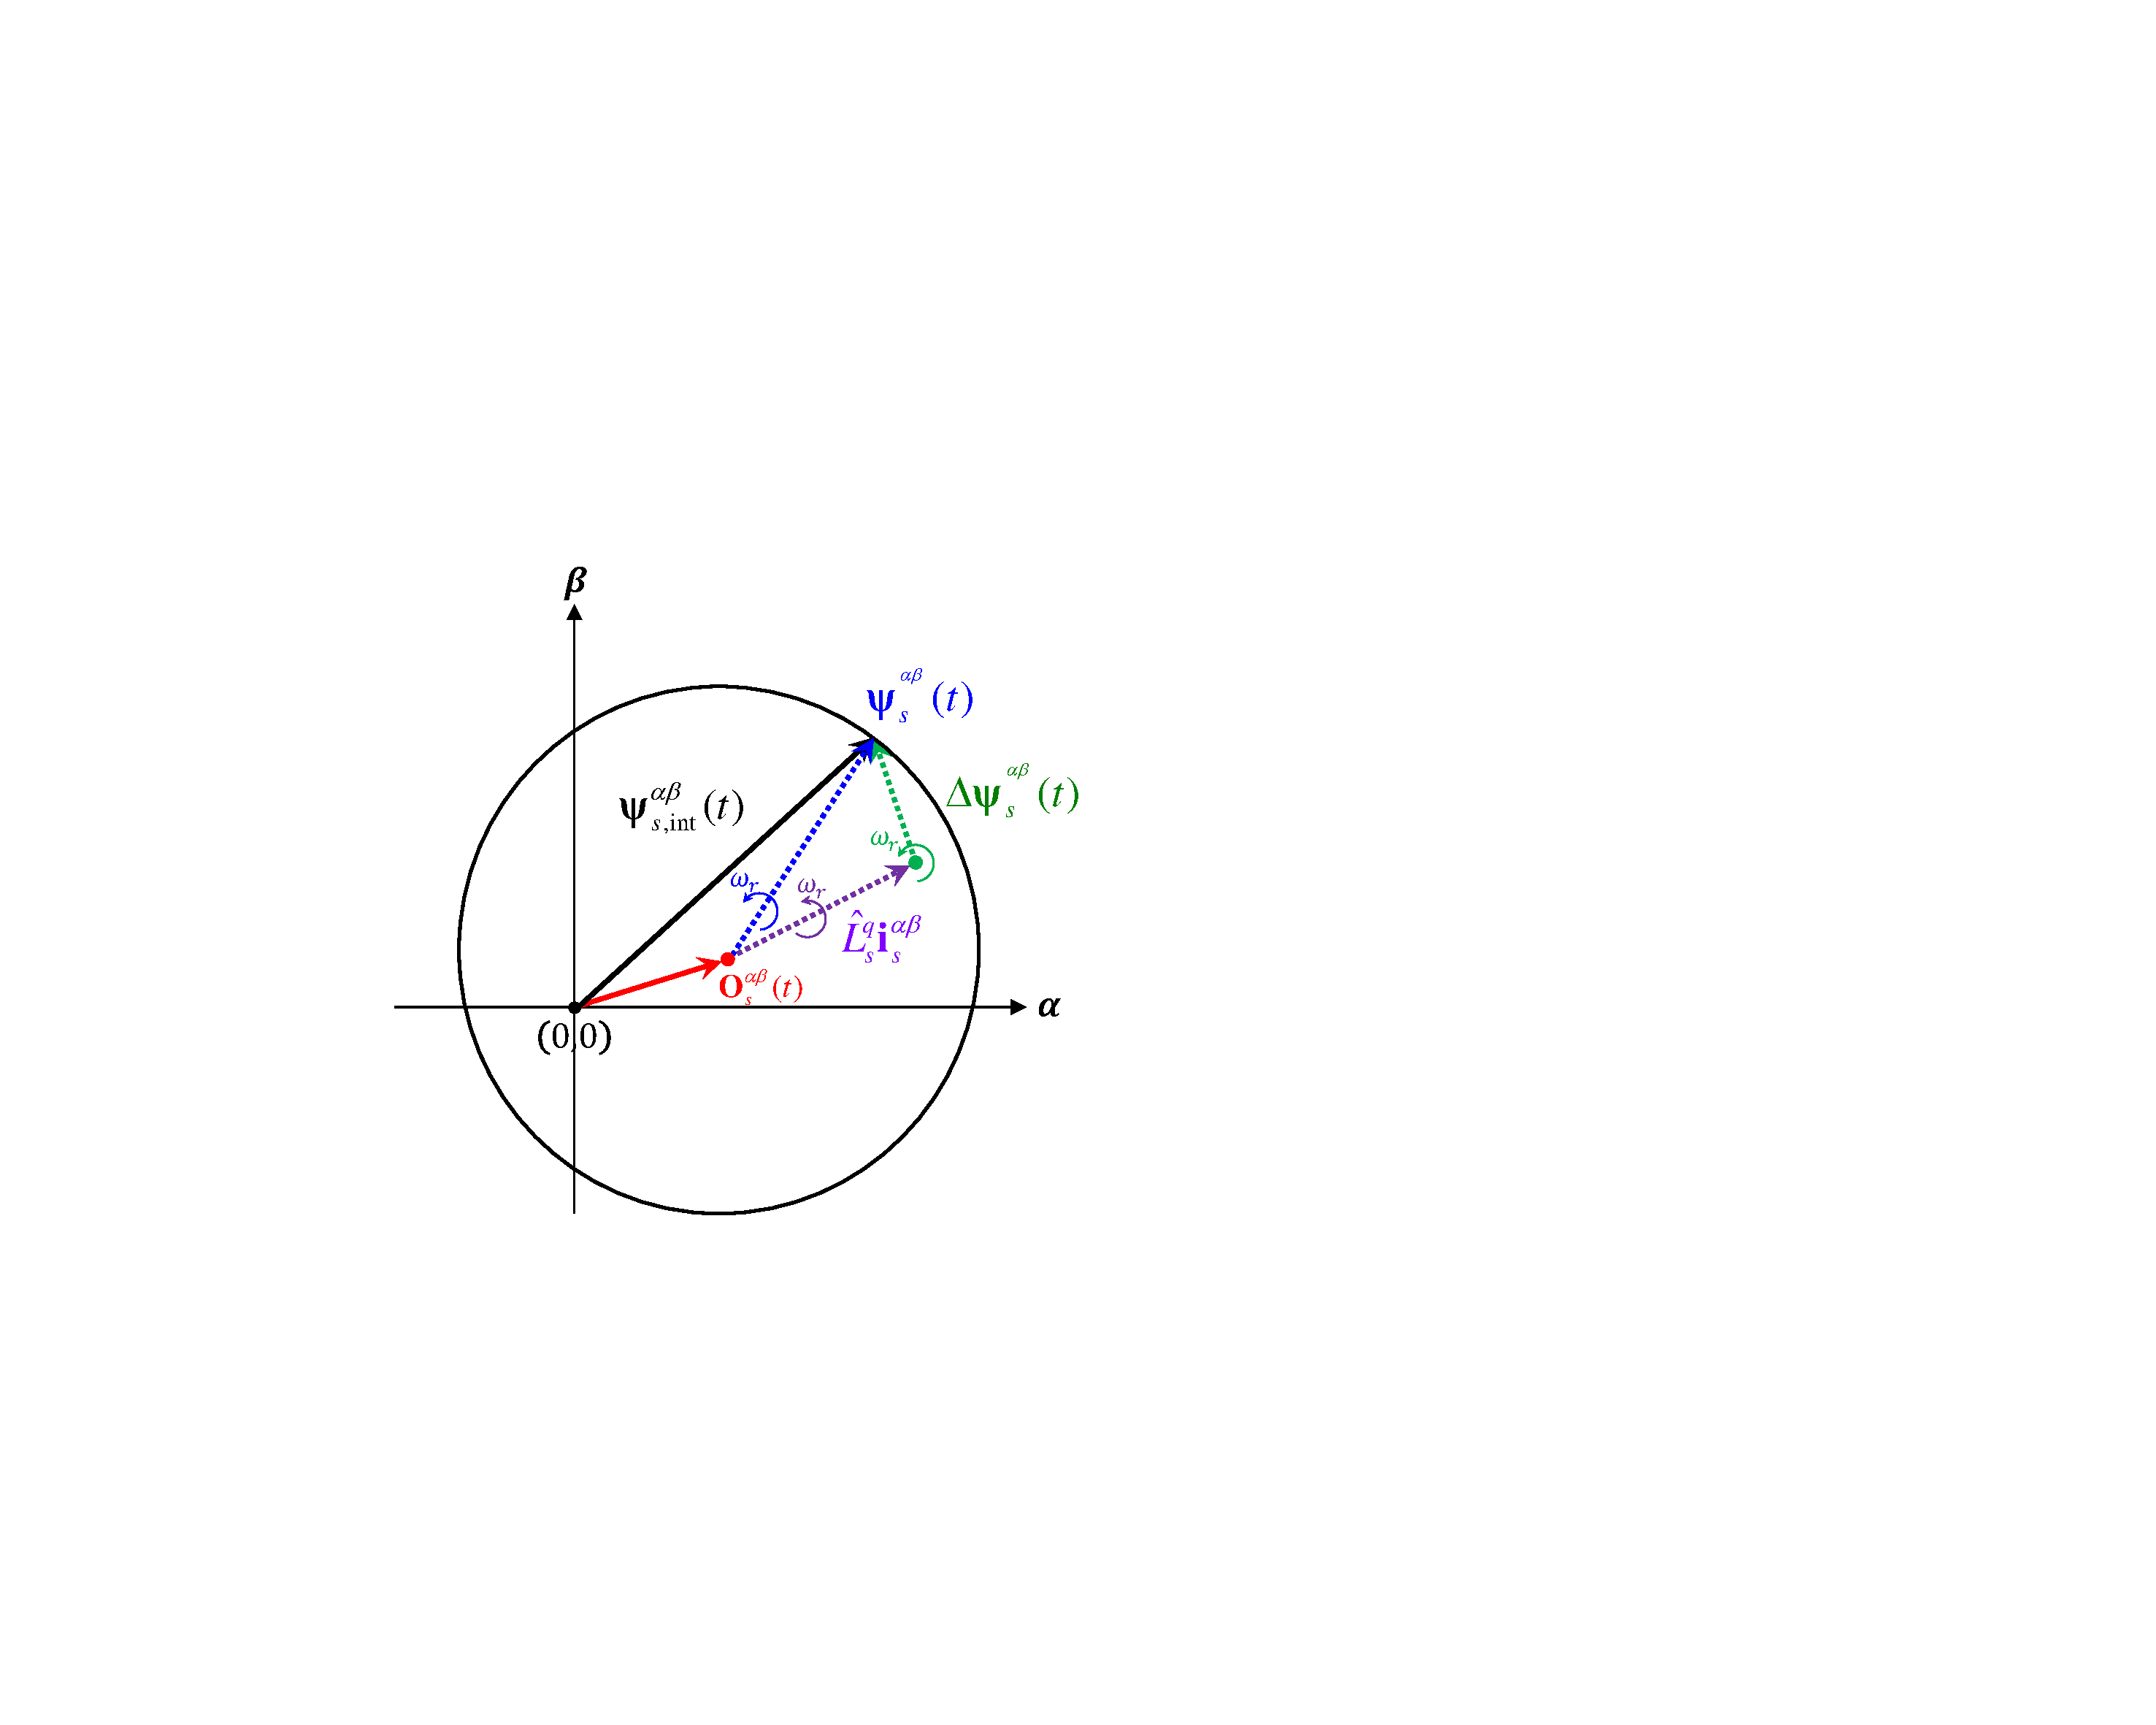
\includegraphics[scale=0.50]{chapters/Fig3.1a.pdf}
    \caption{Components of the integration result $\boldsymbol{\psi}^{\alpha\beta}_{s,\text{int}}$ in steady state.}
    \label{Fig:3.1a}
\end{figure}

\subsubsection{Observable State-Space Model}
By estimating $\Delta\boldsymbol{\psi}^{\alpha\beta}_s$ and ${\mathbf{O}}^{\alpha\beta}_s$ and compensating for the integration error vector ${\mathbf{O}}^{\alpha\beta}_s$ from the integration result vector of (\ref{eqn:3.7}), the stator flux linkage vector $\boldsymbol{\psi}^{\alpha\beta}_s$ can be estimated. Thus, based on (\ref{eqn:3.10}), the state-space model is expressed as
\begin{equation}\label{eqn:3.11}
\left\{
\begin{aligned}
    \frac{d}{dt} \mathbf{x}(t) &= \mathbf{A}(\omega_r) \mathbf{x}(t) + {\mathbf{d}_{t}}(t) \\
    \mathbf{y}(t) &= \mathbf{C} \mathbf{x}(t) + \mathbf{\Psi}(t) \theta(t)
\end{aligned}
\right.
\end{equation}
with
\begin{equation*}
\begin{aligned}
 \mathbf{x} &:= 
\begin{pmatrix}
\boldsymbol{\Delta \psi}^{\alpha\beta}_s \\
\mathbf{O}^{\alpha\beta}_s
\end{pmatrix},
\quad
\mathbf{y} := \boldsymbol{\psi}^{\alpha\beta}_{s,\text{int}}, \quad
\mathbf{d}_t := 
\begin{bmatrix}
\mathbf{d}^{\alpha\beta,\psi}_{s} \\ \mathbf{d}^{\alpha\beta,o}_{s}
\end{bmatrix}, \quad \mathbf{\Psi} := \mathbf{i}_{\alpha\beta},
\quad
\theta:= \hat L_q,
\\
\mathbf{A}(\omega_r) &:= 
\begin{bmatrix}
\omega_r \mathbf{J} & \mathbf{O}_{2\times 2} \\
\mathbf{O}_{2\times 2} & \mathbf{O}_{2\times 2}
\end{bmatrix},
\quad
\mathbf{C} := 
\begin{bmatrix}
\mathbf{I}_{2\times 2} & \mathbf{I}_{2\times 2}
\end{bmatrix}, \quad \mathbf{O}_{2\times2} := \begin{bmatrix}
0  & 0\\
0 & 0
\end{bmatrix}, \quad \mathbf{I}_{2\times2} := \begin{bmatrix}
1  & 0\\
0 & 1
\end{bmatrix},
\end{aligned}
\end{equation*}
where \( \mathbf{x} \) represents the state vector, \( \mathbf{y} \) is the output vector, \( \mathbf{d} \) is the disturbance vector, \( \mathbf{C} \) is the output matrix, \( \mathbf{A}(\omega_r) \) is the time-varying system matrix, \(\mathbf{\Psi}\) represents the current vector in the ($\alpha$,$\beta$)-reference frame, and \(\theta\) denotes an estimate of the $q$-axis inductance parameter, which is updated online to reduce the magnitude of the disturbance vector \(\mathbf{d}\) and improve transient estimation performance. These matrices and vectors are all piecewise continuous and uniformly bounded in time.

To verify whether the dynamic system in (\ref{eqn:3.10}) is observable or not, the observability matrix of the state-space model in (\ref{eqn:3.10}) is given by
\begin{equation}\label{eqn:3.12}
\mathcal{O}(\omega_r) = \begin{bmatrix}
\mathbf{C} \\
\mathbf{C}\mathbf{A}(\omega_r) \\
\mathbf{C}\mathbf{A}(\omega_r)^2 \\
\mathbf{C}\mathbf{A}(\omega_r)^3
\end{bmatrix} = \begin{bmatrix}
\mathbf{I}_{2\times2}& \mathbf{I}_{2\times2} \\
\omega_r \mathbf{J} & \mathbf{O}_{2\times2} \\
(\omega_r \mathbf{J})^2 & \mathbf{O}_{2\times2} \\
(\omega_r \mathbf{J})^3 & \mathbf{O}_{2\times2}
\end{bmatrix},  
\end{equation}
which has a full rank (i.e., \(\mathcal{O}(\omega_r) = 4\)) except for \(\omega_r = 0\), so \(\mathbf{x}\) is fully observable at all constant nonzero electrical angular velocities (as it is slowly varying compared to electrical quantities), similar to the DOB-FLE and ESO-FLE methods. 

\subsubsection{A Liner State Observer Design}
A linear state observer for the state-space model in (\ref{eqn:3.10}) is designed as follows
\begin{equation}\label{eqn:3.13}
\left\{
\begin{aligned}
    \frac{d}{dt} \hat{\mathbf{x}}(t) &= \mathbf{A}(\omega_r) \hat{\mathbf{x}}(t) + \mathbf{F}(\omega_r) \left( \mathbf{y}(t) - \mathbf{C} \hat{\mathbf{x}} - \mathbf{\Psi}(t) \theta(t) \right) \\
    \hat{\mathbf{y}}(t) &= \mathbf{C} \hat{\mathbf{x}}(t) + \mathbf{\Psi}(t) \theta(t)
\end{aligned}
\right.
\end{equation}
where \(\mathbf{\hat{x}}\) and \(\mathbf{\hat{y}}\) represent the estimates of \(\mathbf{x}\) and \(\mathbf{y}\), respectively. The observer gain matrix \(\mathbf{F}(\omega_r) \in \mathbb{R}^{4 \times 2}\) has to be determined with the electrical angular velocity and $\mathbf{A}(\omega_r)$ (i.e. speed-dependant). The dynamic system in (\ref{eqn:3.11}) represents a MIMO (Multi-Input-Multi-Output) system with more variables to estimate than the output equations of the observer. Therefore, \(\mathbf{F}(\omega_r)\) must be designed using eigenstructure assignment as described in \cite{c3.2_2} or robust pole assignment as detailed in \cite{c3.2_3} to accurately place the four closed-loop poles of the observer in (\ref{eqn:3.13}), thus achieving the desired bandwidth of the stable eigenvalues (equivalent to the poles) of the closed-loop observer matrix \(\mathbf{A}(\omega_r) - \mathbf{F}(\omega_r)\mathbf{C}\). In this study, to determine the observer gain matrix \( \mathbf{F}(\omega_r) \), a robust pole assignment method in \cite{c3.2_3} is utilized to place the system poles at the desired (stable) eigenvalues (i.e. establishing a Hurwitz observer matrix \(\mathbf{A}(\omega_r) - \mathbf{F}(\omega_r)\mathbf{C}\) with eigenvalues having negative real parts), which can be calculated using the MATLAB command \texttt{place}. 

Accordingly, by subtracting (\ref{eqn:3.11}) from (\ref{eqn:3.13}), the estimation error dynamics
\begin{equation}\label{eqn:3.14}
\frac{d}{dt} {\mathbf{\tilde{x}}}(t) = \left[ \mathbf{A}(\omega_r) - \mathbf{F}(\omega_r)\mathbf{C} \right] {\mathbf{\tilde{x}}}(t)- {\mathbf{d}_{t}}(t).
\end{equation}
with estimation error $\mathbf{\tilde{x}}:= \mathbf{\hat x}-\mathbf{ x}$ are exponentially stable as the disturbance vector \( \mathbf{d}_{t} \) eventually becomes zero in steady state based on Assumption (A.3.1)$-$(A.3.3).

\begin{figure}[t]
    \centering
    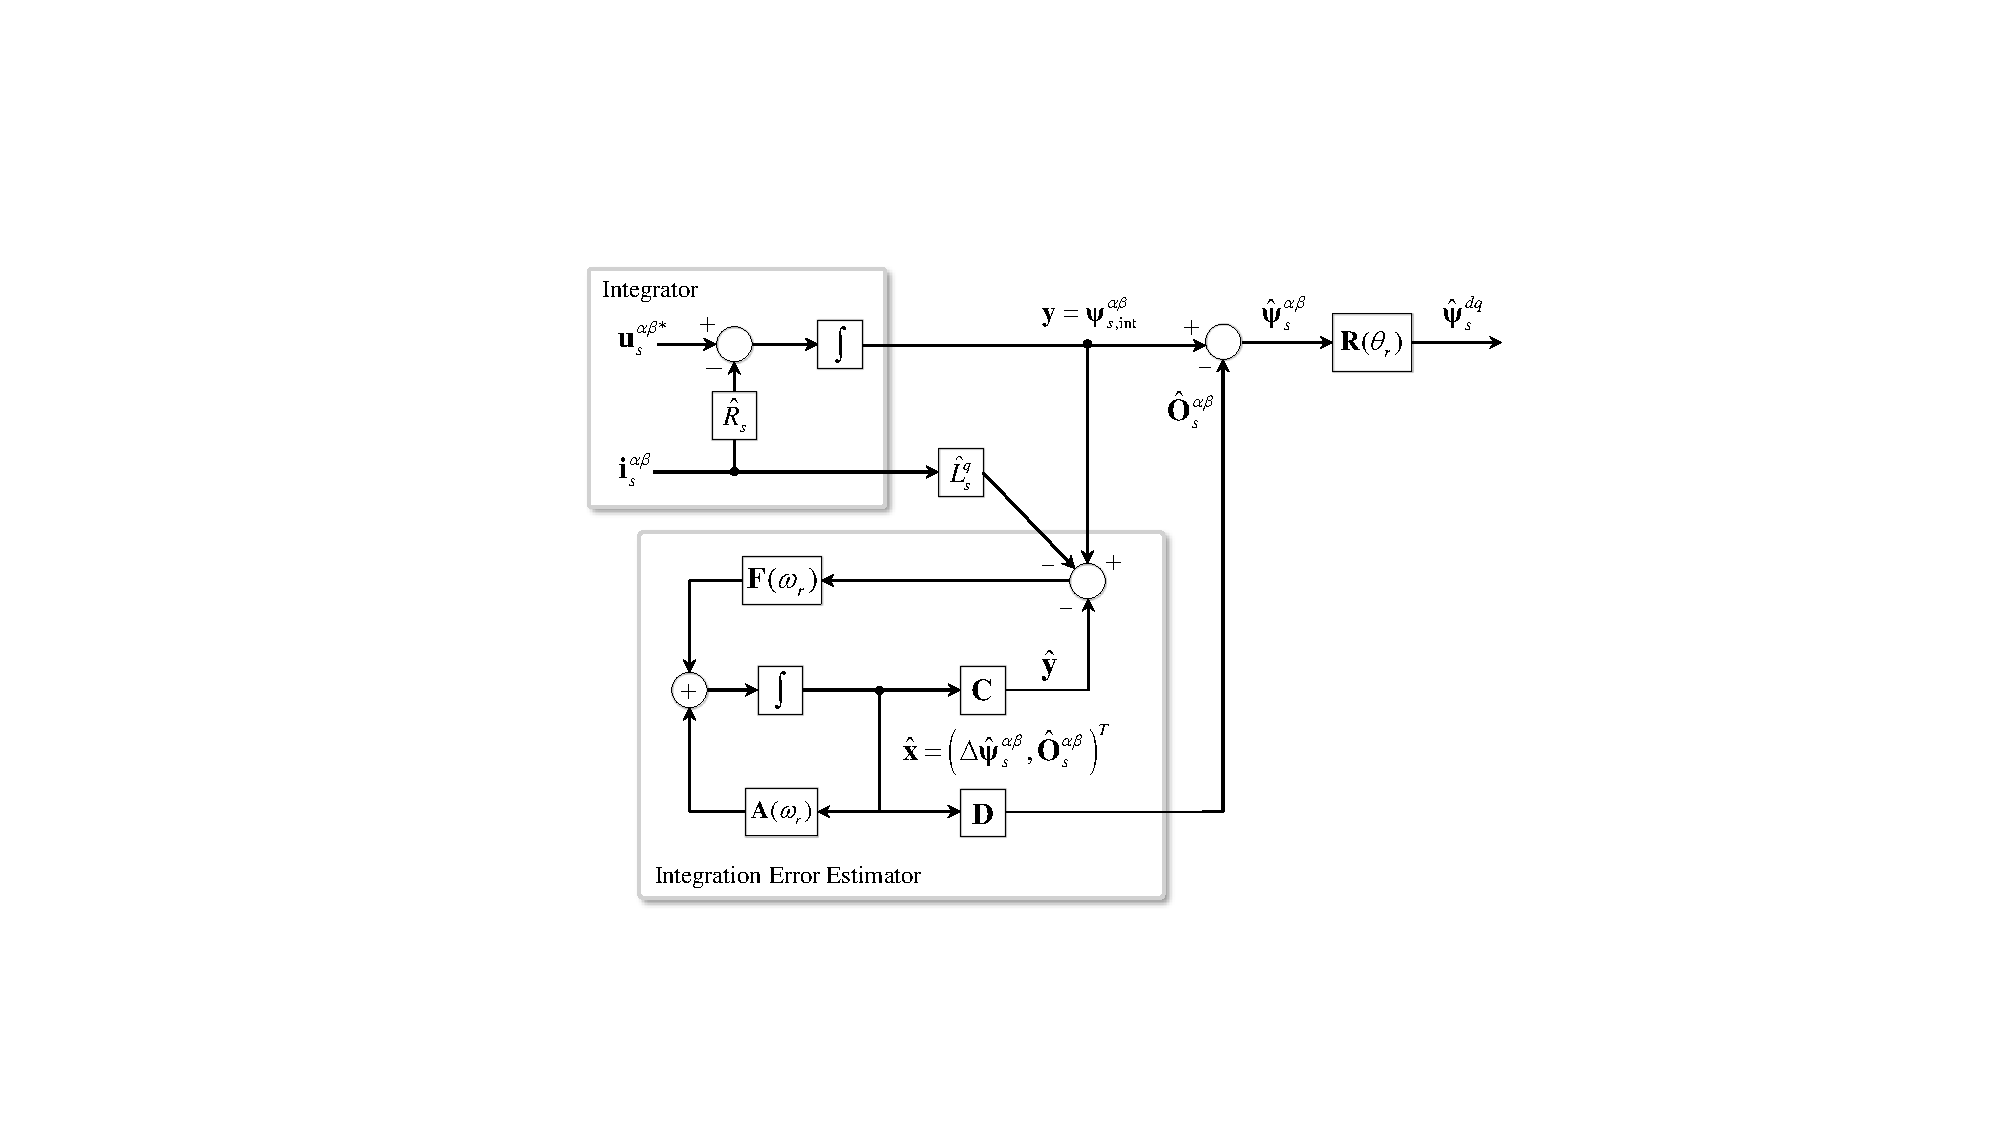
\includegraphics[scale=0.8]{chapters/Fig3.2.pdf}
    \caption{Proposed stator flux linkage estimator based on the integration error estimator}
    \label{Fig:3.2}
\end{figure}

Finally, the estimate of the stator flux linkage vector \( \boldsymbol{\hat{\psi}}^{\alpha\beta}_s \) in the (\(\alpha\),\(\beta\))-reference frame can be obtained by subtracting the integration error estimate \( \boldsymbol{\hat{O}}^{\alpha\beta}_s \) from the integration result \( \boldsymbol{\hat{\psi}}^{\alpha\beta}_{s,\text{int}} \), i.e.
\begin{align}\notag
\boldsymbol{\hat{\psi}}^{\alpha\beta}_s(t) &= \boldsymbol{\hat{\psi}}^{\alpha\beta}_{s,\text{int}}(t) - \boldsymbol{\hat{O}}^{\alpha\beta}_s(t) \\\label{eqn:3.15}
&= \mathbf{y}(t) - \mathbf{D} \boldsymbol{\hat{x}}(t),
\end{align}
with $\mathbf{D} := [\mathbf{O}_{2\times2} \quad \mathbf{I}_{2\times2} ]$. By applying the coordinate transformation in (\ref{eqn:2.8}) to the (\(\alpha,\beta\))-axis estimates in (\ref{eqn:3.15}), the flux estimates in the ($d$,$q$)-reference frame can be obtained as follows
\begin{equation}\label{eqn:3.16}
\boldsymbol{\hat{\psi}}^{dq}_s(t) = \mathbf{R}(\theta_r) \boldsymbol{\hat{\psi}}^{\alpha\beta}_s(t).
\end{equation}

\subsection{Parameter Update for Improving Transient Estimation Performance}
Recalling (\ref{eqn:3.8}) and Assumption (A.3.1), the transient estimation performance of (\ref{eqn:3.16}) depends on the accuracy of the $q$-axis inductance parameter used in the observer of (\ref{eqn:3.13}). Therefore, if the parameter inaccuracy increases, the magnitude of \(\tilde{L}_q\) in (\ref{eqn:3.8}) increases, leading to a larger disturbance vector \(\mathbf{d}^{\alpha\beta,\psi}_s\), which ultimately degrades transient estimation performance. Thus, it is necessary to estimate the $q$-axis inductance online based on the stator current and update it to the actual value to improve transient estimation performance. 

\subsubsection{Parameter Identification Using a Recursive Least-Square Method}
To estimate the parameters online, the Recursive Least Squares (RLS) method with a forgetting factor for continuous time, which is robust to signal noise and inaccuracies, is generally applied \cite{c3.2_4}. For parameter identification, the linear parametric model for the $q$-axis flux linkage can be expressed as
\begin{equation}\label{eqn:3.17}
    \psi^q_s(t) = L^q_s(t)i^q_s(t), \quad \hat\psi^q_s(t) \rightarrow \psi^q_s(t) \text{ as t } \rightarrow \infty,
\end{equation}
where the flux estimate \(\hat \psi^q_s\) is used as the output of the linear parametric model since the $q$-axis flux linkage \(\psi^q_s\) cannot be directly measured (the estimation error \(\mathbf{\tilde{x}}\) asymptotically converges to the zero vector \(\mathbf{O}_2\) as \(t \rightarrow \infty\)). To estimate the unknown $q$-axis inductance parameter, the linear model in (\ref{eqn:3.17}) is rearranged as follows
\begin{equation}\label{eqn:3.18}
\begin{aligned}
z &= \theta^* u = \hat\psi^q_s(t), \ \theta^* = L^q_s(t), \ u = i^{q}_s(t),
\end{aligned}
\end{equation}
where \(z\) represents the output signals of the parametric model, \(\theta^*\) is the unknown parameter to be estimated, and \(u\) represents the input signals, respectively. The estimate of $z$ in (\ref{eqn:3.18}) can be expressed as  
\begin{equation}\label{eqn:3.19}
\hat{z} = \theta u, \ \theta = \hat{L}^q_s(t),
\end{equation}
where \(\hat{z}\) and \(\theta\) denote the estimate of \(z\) and the estimated parameter of \(\theta^*\), respectively and the parameter estimation error
\begin{equation}\label{eqn:3.20}
\epsilon =z - \hat{z} = z - \theta u
\end{equation}
can be derived. Therefore, to minimize the parameter estimation error in (\ref{eqn:3.20}) and identify the parameter $\theta$ using a convex integral objective function, the continuous-time recursive least-squares parameter update algorithm (see Appendix \ref{Appen1})
\begin{equation}\label{eqn:3.21}
\begin{aligned}
\dot{\theta} &= \Gamma \epsilon^\top u \\
    \dot{\Gamma} &= \beta \Gamma - \Gamma u^\top u \Gamma
\end{aligned}
\end{equation}
with the covariance $\Gamma$ and the forgetting factor $\beta$. Therefore, if the input signal \(u\) satisfies the PE (Persistent Excitation) condition and \(\theta\) and \(\dot{\theta}\) are uniformly bounded, then \(\theta\) will eventually converge exponentially to the actual parameter \(\theta^*\). Therefore, by using the RLS algorithm in (\ref{eqn:3.21}) to update the $q$-axis inductance parameter in the observer of (\ref{eqn:3.13}) online, the transient estimation performance can be improved.

\subsubsection{Adaptive Observer based on the Parameter Update}
The flux estimation error made by the inductance parameter (\(\hat{L}^q_s\)) update in (\ref{eqn:3.21}) can be compensated for by an adaptive observer that adds an auxiliary term to the flux estimation dynamics. The $\alpha$-$\beta$ axis rotating nonlinear flux linkage vector $\Delta \boldsymbol{\psi}^{\alpha \beta}_s$ in (\ref{eqn:3.6a}) can be redefined as
\begin{align}\label{eqn:3.23}
\boldsymbol{\psi}^{\alpha\beta}_s(t) = L^q_s(t) \mathbf{i}^{\alpha\beta}_s(t) + 
\underbrace{\mathbf{P}(\theta_r)
\Delta \psi^{d}_s(t)}_{=:\Delta \boldsymbol{\psi}^{\alpha \beta}_s(t)},
\end{align}
where the time derivative of the rotating nonlinear flux in (\ref{eqn:3.23}) leads
\begin{equation}\label{eqn:3.24}
\begin{aligned}
\frac{d}{dt}{\boldsymbol{\Delta \psi}}^{\alpha\beta}_s(t) &= \omega_r(t) \mathbf{J}\underbrace{\mathbf{P}(\theta_r)\Delta \psi^{d}_s(t)}_{\stackrel{(\ref{eqn:3.23})}=\Delta\boldsymbol{\psi}^{\alpha\beta}_s}+\underbrace{\mathbf{P}(\theta_r) \Delta \dot\psi^{ d}_s(t)}_{=:\mathbf{d}^{\alpha\beta,\psi}_{s}(t)}
\\
&= \omega_r(t) \mathbf{J} \Delta \boldsymbol{\psi}^{\alpha\beta}_s(t) + \mathbf{d}^{\alpha\beta,\psi}_{s}(t)
\end{aligned},
\end{equation}
where the disturbance vector \(\mathbf{d}^{\alpha\beta,\psi}_s\) converges to zero in steady state, recalling Assumption (A.2.2). Accordingly, the output ($\boldsymbol{\psi}^{\alpha\beta}_{s,\text{int}}$) and dynamics ($\Delta \dot{\boldsymbol{\psi}}^{\alpha \beta}_s$,$\dot{\mathbf{O}}^{\alpha\beta}_s$) are summarized as follows
\begin{equation}
\begin{aligned}\label{eqn:3.25}
\begin{cases}
\frac{d}{dt}{\Delta \boldsymbol{\psi}}^{\alpha\beta}_s(t) = \omega_r(t) \mathbf{J} \Delta \boldsymbol{\psi}^{\alpha\beta}_s(t) + \mathbf{d}^{\alpha\beta,\psi}_{s}(t) \\
\frac{d}{dt}{\mathbf{O}}^{\alpha\beta}_s(t) = \mathbf{d}^{\alpha\beta,o}_{s}(t) \\
\boldsymbol{\psi}^{\alpha\beta}_{s,\text{int}}(t) = L^q_s(t) \mathbf{i}^{\alpha\beta}_s(t) + 
\Delta \boldsymbol{\psi}^{\alpha \beta}_s(t) + \mathbf{O}^{\alpha\beta}_s(t)
\end{cases}
\end{aligned},
\end{equation}
where the state-space model in (\ref{eqn:3.25}) is the same as (\ref{eqn:3.11}) except for \(\theta := L^q_s\). Thus, an adaptive observer 
\begin{equation}\label{eqn:3.26}
\left\{
\begin{aligned}
    \frac{d}{dt} \hat{\mathbf{x}}(t) &= \mathbf{A}(\omega_r) \hat{\mathbf{x}} + \mathbf{F}(\omega_r) \left( \mathbf{y}(t) - \mathbf{C} \hat{\mathbf{x}}(t) - \mathbf{\Psi}(t) \hat\theta(t) \right) + \mathbf{w}(t) \\
    \hat{\mathbf{y}}(t) &= \mathbf{C} \hat{\mathbf{x}}(t) + \mathbf{\Psi}(t) \hat{\theta}(t)
\end{aligned}
\right.
\end{equation}
can be designed, where \(\theta := L_q\) is an unknown actual inductance parameter and \(\mathbf{w}\) is an auxiliary term in order to compensate the estimation error made by parameter estimate $\hat\theta$. Since there are no changes in the \( \mathbf{A}(\omega_r) \) and \( \mathbf{C} \) matrices, the rank of the observability matrix remains the same in (\ref{eqn:3.11}), ensuring that all states can be observed. By subtracting (\ref{eqn:3.11}) from  (\ref{eqn:3.26}), the estimation error dynamics
\begin{equation}\label{eqn:3.27}
\frac{d}{dt} \tilde{\mathbf{x}}(t) = \left[ \mathbf{A}(\omega_r) - \mathbf{F}(\omega_r)\mathbf{C} \right] \tilde{\mathbf{x}}(t) - \mathbf{F}(\omega_r)\mathbf{\Psi}(t) \tilde\theta(t) + \mathbf{w}(t) - {\mathbf{d}_{t}}(t)
\end{equation}
with the parameter estimation error \(\tilde{\theta} := \hat{\theta} - \theta\). To design an adaptation law that compensates for the term \(\mathbf{F}(\omega_r)\mathbf{\Psi}\tilde\theta\), which affects the convergence of the estimation error dynamics in (\ref{eqn:3.27}) due to parameter estimation error, with an auxiliary term \(\mathbf{w}\), the following assumption is introduced \cite{c3.2_5}.

\textbf{Assumption (A.3.4)} The state estimation error \(\tilde{\mathbf{x}}\), parameter estimation error \(\tilde{\theta}\), and the time-varying matrix \(\boldsymbol{\Upsilon}\) can be expressed as a linear combination of \(\boldsymbol{\eta}\) \cite{c3.2_6} as follows
\begin{equation}\label{eqn:3.28}
\boldsymbol{\eta}(t) = \tilde{\mathbf{x}}(t) - \boldsymbol{\Upsilon}(t) \tilde{\theta}(t),
\end{equation}

Considering Assumption (A.3.4), the time derivative of (\ref{eqn:3.28}) can be expressed as 
\begin{align}\label{eqn:3.29}
\frac{d}{dt}{\boldsymbol{\eta}}(t) &= \dot{\tilde{\mathbf{x}}}(t) - \mathbf{\Upsilon}(t) \dot{\tilde{\theta}}(t) - \dot{\mathbf{\Upsilon}}(t) \tilde{\theta}(t) \\\notag
&= \underbrace{(\mathbf{A}(\omega_r) - \mathbf{F}(\omega_r)\mathbf{C})}_{:= \mathbf{A}_c} \tilde{\mathbf{x}}(t) - \mathbf{F}(\omega_r)\mathbf{\Psi}(t) \tilde{\theta}(t) +\mathbf{w}(t) - {\mathbf{d}_{t}}(t) 
-\mathbf{\Upsilon} \dot{\tilde{\theta}}(t) - \dot{\mathbf{\Upsilon}} \tilde{\theta}(t) \\\notag
&= \mathbf{A}_c {\boldsymbol{\eta}}(t)+ \left[ \mathbf{A}_c \mathbf{\Upsilon}(t) - \mathbf{F}(\omega_r)\mathbf{\Psi}(t) - \dot{\mathbf{\Upsilon}}(t) \right] \tilde{\theta}(t) + \mathbf{w}(t) - \mathbf{\Upsilon}(t) \dot{\tilde{\theta}}(t) 
- {\mathbf{d}_{t}}(t)
\end{align}
where \(\dot{\theta}\) becomes zero as \( t \rightarrow \infty \). Therefore, to make the equation in (\ref{eqn:3.29}) stable, the \(\tilde{\theta}\) and \(\dot{\tilde{\theta}}\) terms can be eliminated by
\begin{equation}\label{eqn:3.30}
\begin{aligned}
\dot{\mathbf{\Upsilon}}(t) &= \mathbf{A}_c \mathbf{\Upsilon}(t) - \mathbf{F}(\omega_r) \mathbf{\Psi}(t)\\
    \mathbf{w}(t) &= \mathbf{\Upsilon}(t) \dot{\tilde{\theta}}(t)=\mathbf{\Upsilon}(t)\dot{\hat{\theta}}(t)
\end{aligned},
\end{equation}
where the equation in (\ref{eqn:3.29}) can be rearranged as 
\begin{align}\label{eqn:3.31}
\dot{\boldsymbol{\eta}}(t) &=  \mathbf{A}_c \boldsymbol{\eta}(t) 
- {\mathbf{d}_{t}}(t).
\end{align}
If the observer matrix \(\mathbf{A}_c\)  becomes Hurwitz (stable) and under Assumption (A.2.2) and Assumption (A.3.3) (${\mathbf{d}_{t}}\rightarrow 0$ as $ t \rightarrow \infty$) in steady state, \(\boldsymbol{\eta}\) is exponentially stable, resulting in \(\hat{x} \rightarrow x\) and \(\hat{\theta} \rightarrow \theta\). The adaptive algorithm for the adaptive observer based on the parameter update is summarized as follows
\begin{equation}\label{eqn:3.34}
\left\{
\begin{aligned}
\dot{\mathbf{\Upsilon}}(t) &= \mathbf{A}_c \mathbf{\Upsilon}(t) - \mathbf{F}(\omega_r) \mathbf{\Psi}(t)\\
    \mathbf{w}(t) &=\mathbf{\Upsilon}(t)\dot{\hat{\theta}}(t)
    \\
        \dot{\hat\theta} &= \Gamma \epsilon^\top u\\
    \dot{\Gamma} &= \beta \Gamma - \Gamma u^\top u \Gamma
\end{aligned},
\right.
\end{equation}
with
\begin{equation*}
z = \hat\psi^q_s(t),\quad u = i^q_s, \quad \hat{\theta} = \hat{L}^q_s(t) , \quad \epsilon =z - \hat{\theta}u.
\end{equation*}

Therefore, the proposed adaptive observer compensates for the flux estimation error caused by the inductance parameter error estimated by RLS by adding an auxiliary term \(\mathbf{w}\) to the estimation dynamics through an adaptation law. This approach reduces the norm of the disturbance vector \(\|\mathbf{d}^{\alpha\beta,\psi}_s\|\), improving transient estimation performance and ensuring robustness against parameter variations in the observer.

\end{spacing}
%%%%%%%%%%%%%%%%%%%%%%%%%%%%%%%%%%%%
% Chapter 4 Simulation Validations
%%%%%%%%%%%%%%%%%%%%%%%%%%%%%%%%%%%%

\begin{spacing}{2.0}

\chapter{Simulation Validations}\label{chapter4}
\subsubsection{Simulation Setup}
To verify the estimation performance of the two proposed flux estimators, the `\texttt{Three-phase PMSM Traction Drive}' example for the 35kW IPMSM provided by MATLAB/Simulink (R2023b), which utilizes the FEM-parameterized PMSM library, was used. Figure \ref{Fig:4.1} shows the overall simulation environment of the PMSM, where the controller was modified for the flux linkage estimator and the FCS-MPC current controller. The simulation specifications and flux linkage maps are listed in Table \ref{Tab4.1} and shown in Fig.\ref{Fig:4.2}. 
To implement FCS-MPC-based current control, \begin{figure}[h]
    \centering
    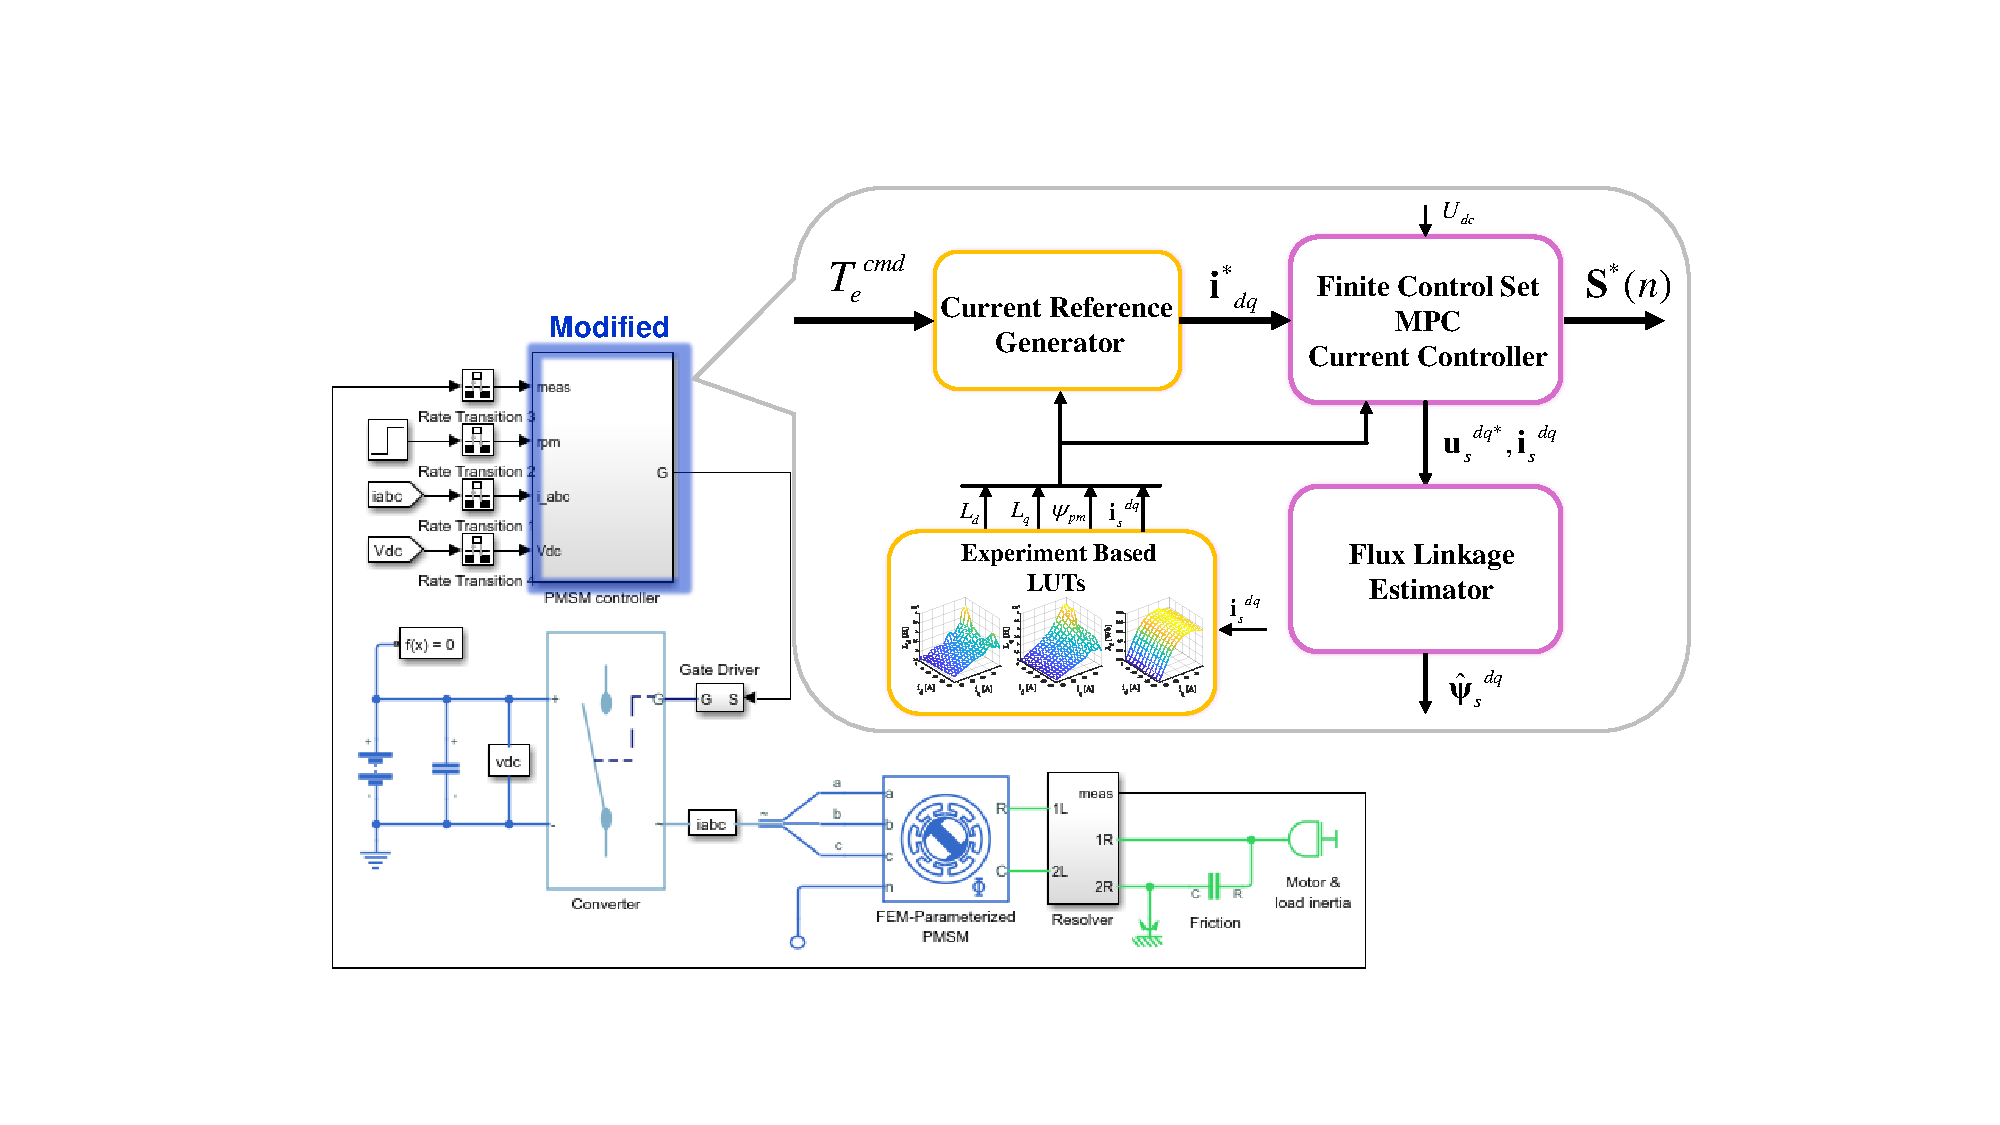
\includegraphics[scale=0.53]{chapters/Fig4.1.pdf}
    \caption{MATLAB/Simulink simulation environment for IPMSM control}
    \label{Fig:4.1}
\end{figure}a numerical reference generator presented in \cite{c1_2} was used to convert the torque command into current references. Additionally, the sampling time for the sensors was set to 20 kHz, and the sampling time for the flux linkage estimator and FCS-MPC switching calculation was set to 40 kHz. The period for the torque generator was set to 1 kHz. These control periods were determined using the \texttt{"state flow"} library provided by MATLAB/Simulink. 
\begin{table}[t]
\caption{Specifications of the IPMSM Drive}\label{Tab4.1}
\centering
\begin{tabular}{l r}
\toprule
\hline
\textbf{Parameter} & \textbf{Value}  \\ \midrule
Base speed & 2000 rpm \\
Maximum torque & 180 Nm\\
DC-link voltage ($U_{\text{dc}}$) & 325 V \\
Maximum stator current ($I_{\text{max}}$) & 350 A \\
Rotor Inertia & 0.1234 kg\,m$^2$ \\
Number of pole pairs ($n_p$) & 8\\
Stator winding resistance ($R_s$) & 10.9 m$\Omega$\\
Time sampling ($T_s$) & 25 $\mu$s \\
\hline
\bottomrule
\end{tabular}
\end{table}
\begin{figure}[t]
    \centering
    \begin{subfigure}[c]{0.47\textwidth}
        \centering
        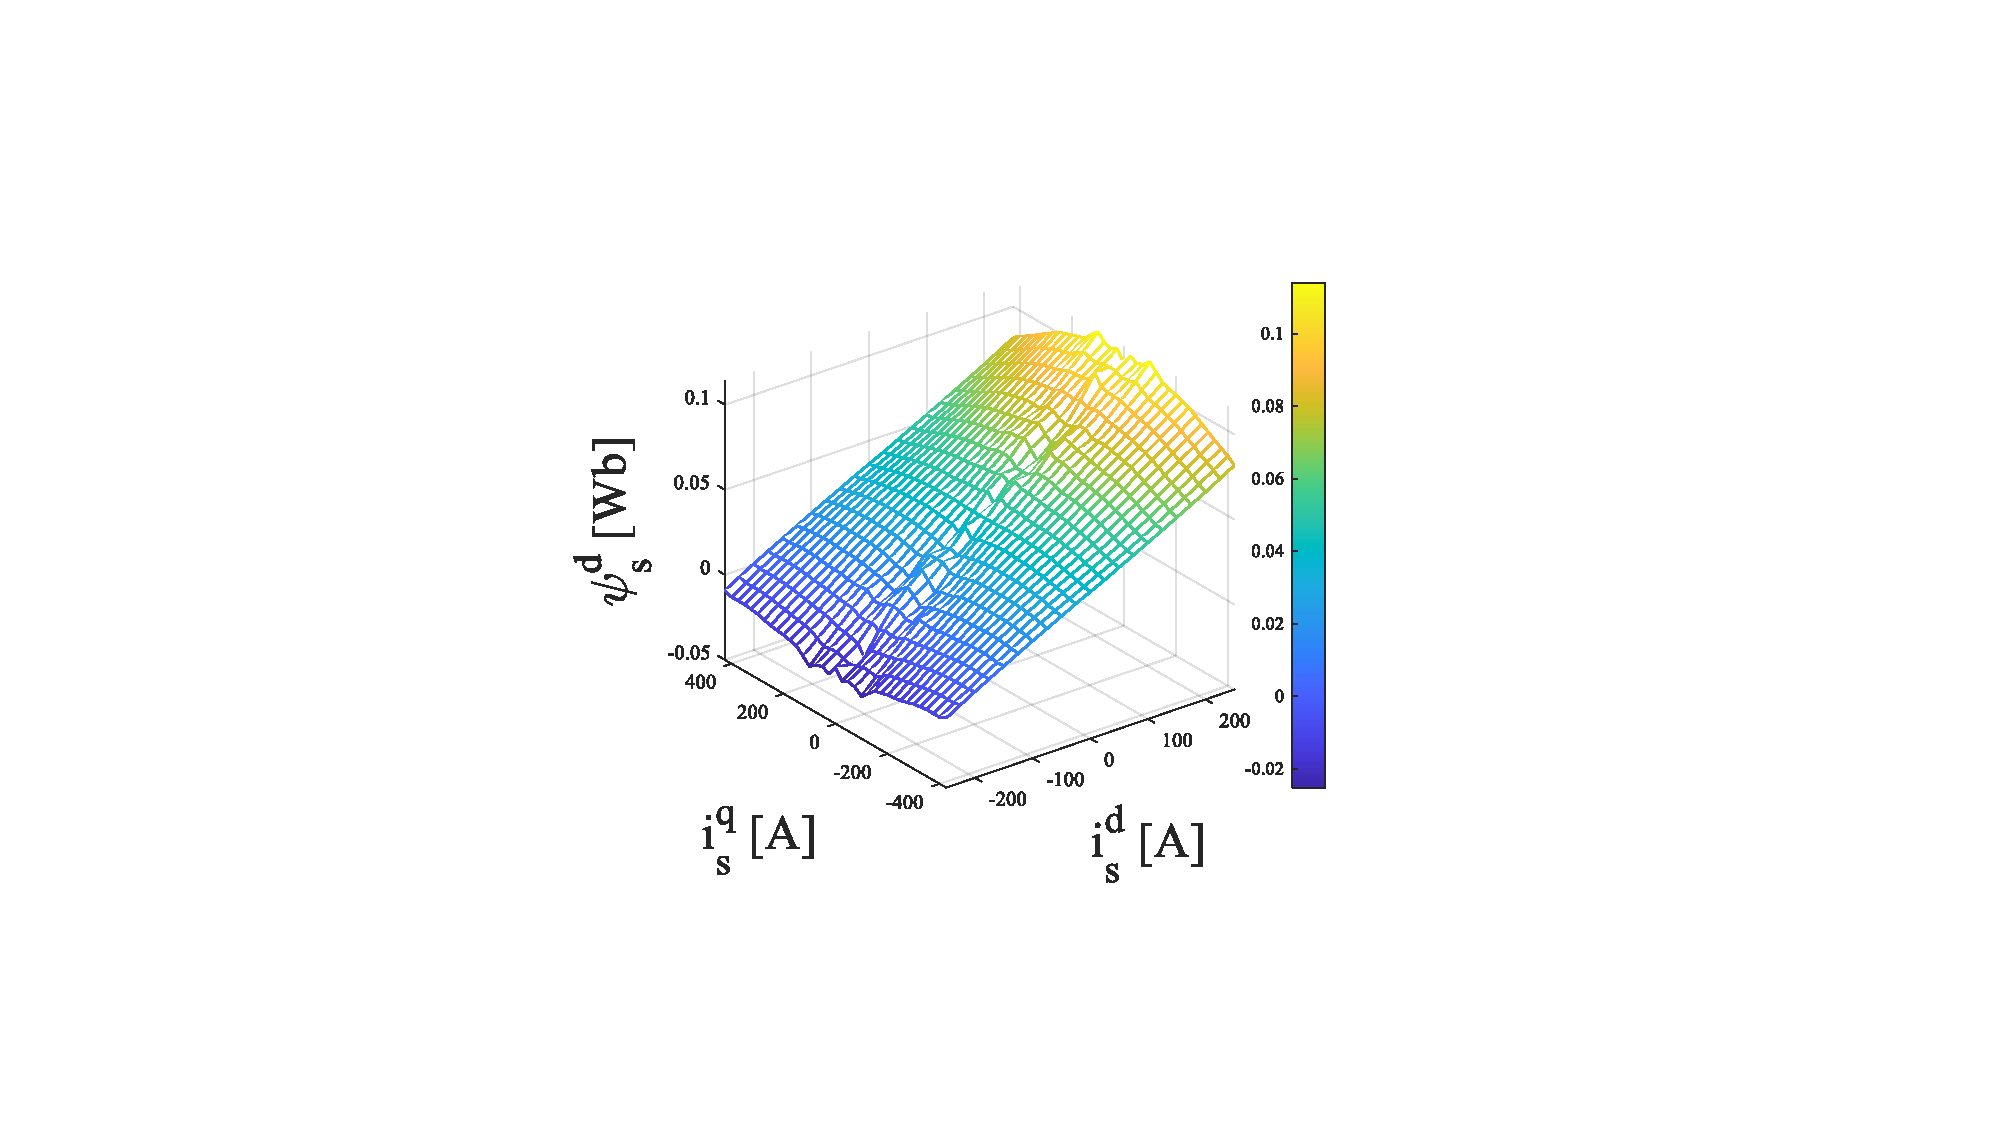
\includegraphics[scale=0.5]{chapters/Fig4.2a.pdf}
        \caption{}
        \label{Fig:4.2a}
    \end{subfigure}
    \hfill
    \begin{subfigure}[c]{0.47\textwidth}
        \centering
        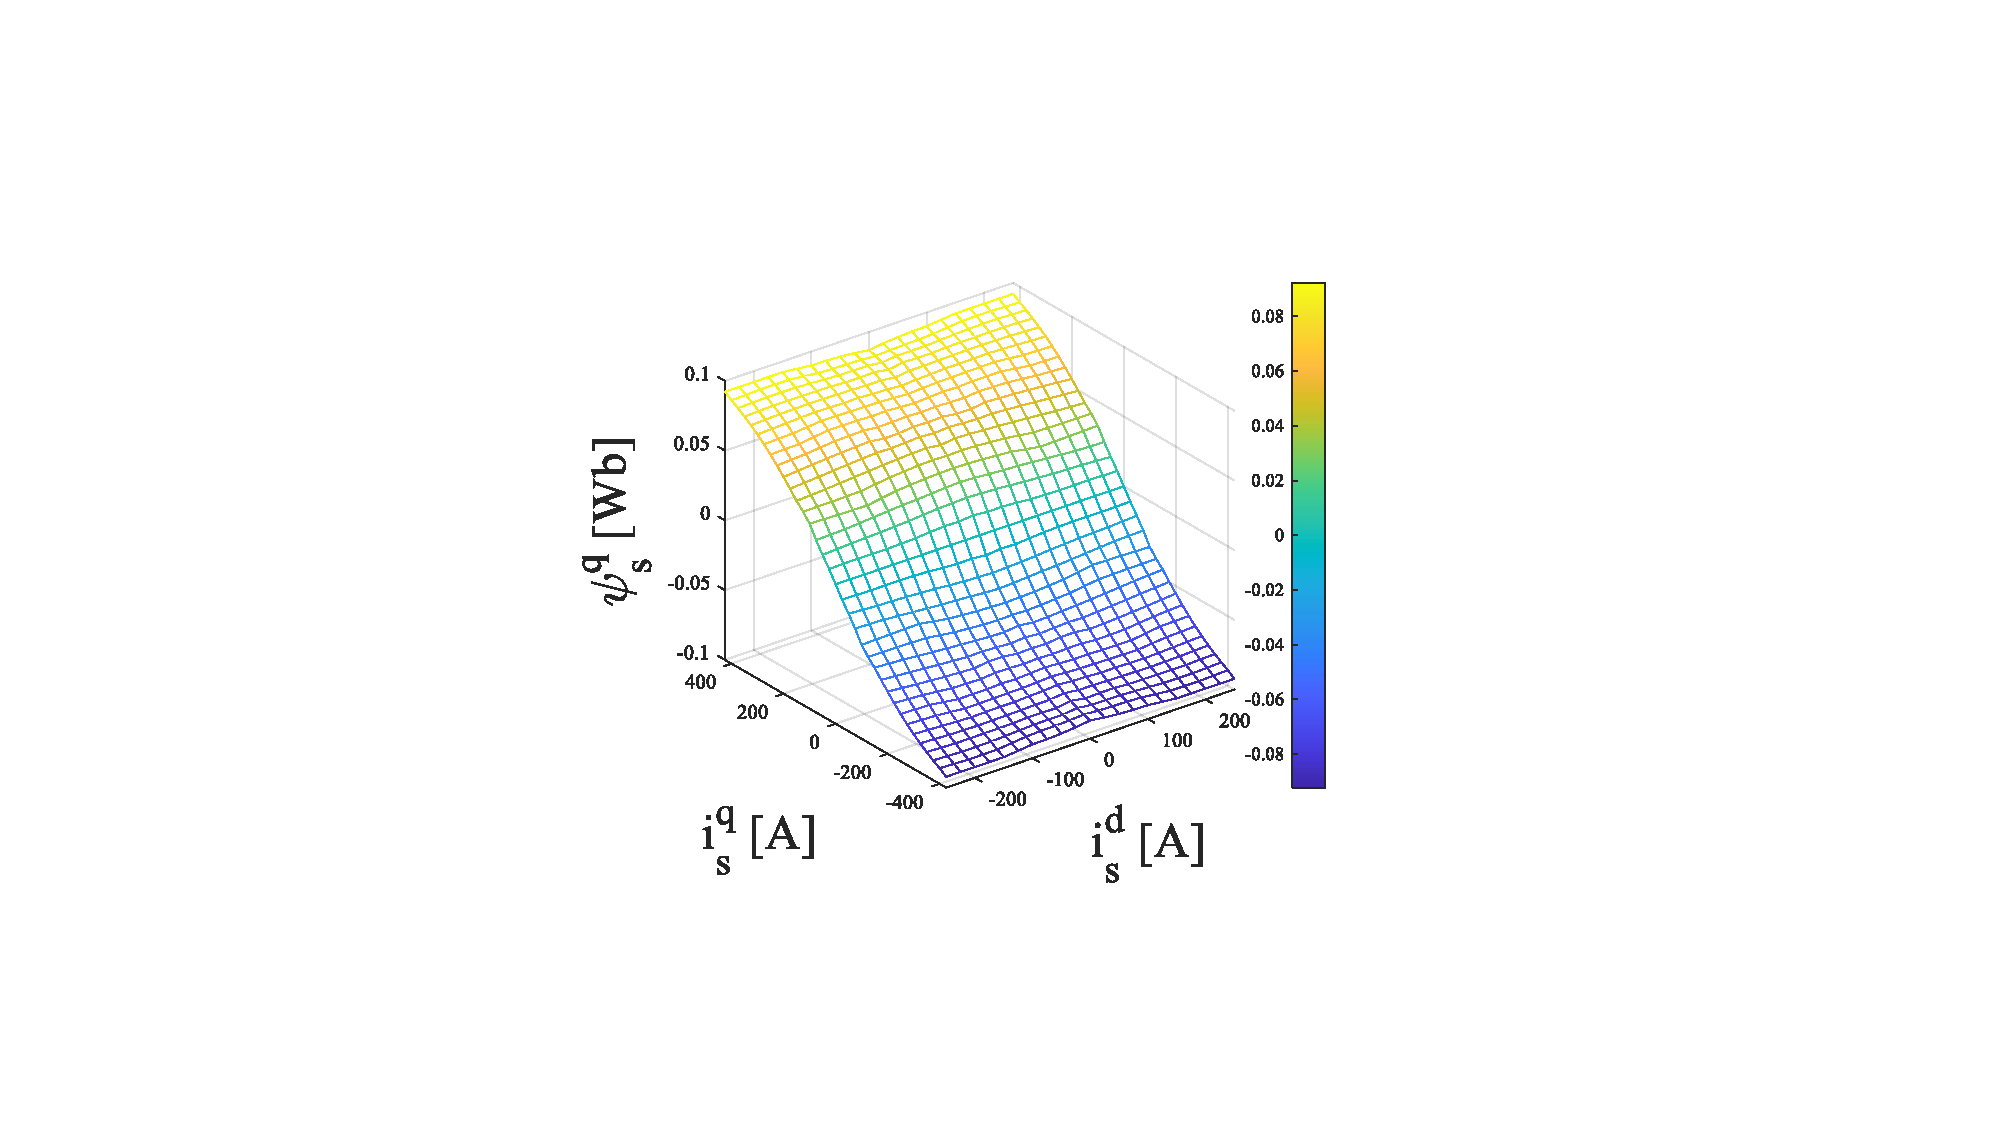
\includegraphics[scale=0.5]{chapters/Fig4.2b.pdf}
        \caption{}
        \label{Fig:4.2b}
    \end{subfigure}
    \caption{Nonlinear flux linkage maps of the IPMSM (a) $d$-axis and (b) $q$-axis.}
    \label{Fig:4.2}
\end{figure}

To determine the gain matrices ${{\boldsymbol{F}({\omega}_{r})}}$ of all state observers (DOB-FLE, ESO-FLE, and IE-PU-FLE) used for simulation verification, a robust pole assignment method \cite{c3.2_3} was utilized to place the system poles at the desired (stable) eigenvalues. This can be easily achieved by using the MATLAB command \texttt{"place"} to calculate the gain matrix ${{\boldsymbol{F}({\omega}_{r})}}$. Additionally, the feedback gain matrix ${{\boldsymbol{F}({\omega}_{r})}}$ was designed so that the bandwidth of the stable eigenvalues of the matrix ${{\boldsymbol{A}}({\omega}_{r})} - {{\boldsymbol{F}({\omega}_{r})}} {{\boldsymbol{C}}}$ is approximately 100 Hz (628 rad/s) at a constant mechanical speed of 500 RPM for all flux linkage estimators. This bandwidth was chosen to be about twice the settling time (50 Hz) of the torque reference command, considering the estimation performance.

\section{Validation of the Proposed ESO-FLE}
The simulation scenarios for verifying the estimation performance of the proposed ESO-FLE are as follows: (i) The estimation performance was verified using nominal inductance ($\mathbf{L}^{dq}_{s,0}$), with the mechanical speed varying from 200 RPM to 1300 RPM and the torque changing from -180 Nm to 180 Nm (In Fig. \ref{Fig:4.3}). (ii) The transient estimation performance was examined using the guessed nominal inductance ($\hat{\mathbf{L}}^{dq}_{s,0}:=0.5\mathbf{L}^{dq}_{s,0}$), with a fixed speed of 500 RPM \begin{table}[h]
\caption{Observer parameters for ESO-FLE}\label{Tab4.2}
\centering
\begin{tabular}{l c}
\hline
\textbf{Parameter} & \textbf{Value}  \\ \midrule
Feedback gain matrix & $\mathbf{F}(419\frac{\text{rad}}{\text{s}})=\begin{bmatrix}
    0.0782 & -0.6481\\
    0.6565 & 0.0919\\
    -0.4008 & -0.7540\\
    0.7599 & -0.3822\\
    -1.4033 & -162.11\\
    166.06 & 1.2415
\end{bmatrix}$\\
\\
Nominal inductance & $\mathbf{L}^{dq}_{s,0}=\begin{bmatrix}
    0.25 & 0\\
    0 & 0.28
\end{bmatrix}$mH\\
\\
\textit{Guessed} nominal inductance & $\hat{\mathbf{L}} ^{dq}_{s,0}= 0.5\times\begin{bmatrix}
    0.25 & 0\\
    0 & 0.28
\end{bmatrix}$mH\\
\\
\hline
\end{tabular}
\end{table}and the torque increasing from 0 to 180 Nm (In Fig. \ref{Fig:4.9}). In all scenarios, a gain matrix selected for a constant mechanical speed of 500 RPM was used for the estimation. The observer parameters used to verify the estimation performance of the proposed ESO-FLE are listed in Tab. \ref{Tab4.2} 

Figure \ref{Fig:4.3} shows the flux linkage estimates, their estimation errors \(\boldsymbol{e}_s := \boldsymbol{\psi}^{dq}_s - \hat{\boldsymbol{\psi}}^{dq}_s\), and the operating conditions of the proposed ESO-FLE. At $t = 0.05$ seconds, when the electrical torque starts increasing to 180 Nm, a large spike-like estimation error occurred in the flux estimates during the transient state (during $t=0.05$ s and $t=0.07$ s). This is because the observer gain matrix \(\mathbf{F}(\omega_r)\) was designed for a constant speed of 500 rpm rather than varying with the mechanical speed, making the observer gain sensitive in the low-speed region and affecting the estimation performance. However, above 200 RPM, the flux linkage estimates closely tracked their true values under dynamic operating conditions across a wide range of torque (-180 Nm to 180 Nm) and speed (200 RPM to 1300 RPM). Thus, the simulation results in Fig. \ref{Fig:4.3} demonstrated that the proposed ESO-FLE shows good estimation performance in both transient and steady states over a wide operating range using nominal inductance, thereby validating its effectiveness.

Figure \ref{Fig:4.9a} shows the transient estimation performance results at a constant speed of 500 RPM using the guessed nominal inductance, and Figure \ref{Fig:4.9b} shows the estimation error norm $||\mathbf{e}_s||$, which quantitatively represents the estimation performance. Here, because the finite control set MPC method directly determines the $d$-axis and $q$-axis voltage inputs for the $d$-axis and $q$-axis current references, respectively, it seems that the flux estimates include significant switching ripples in their estimation error norms. \begin{figure}[!h]
    \centering
    \includegraphics[scale=2.1]{chapters/Fig4.3.pdf}
    \caption{Flux linkage estimates of the proposed ESO-FLE}
    \label{Fig:4.3}
\end{figure} \begin{figure}[h!]
    \centering
    \begin{subfigure}[c]{1.0\columnwidth}
        \centering
        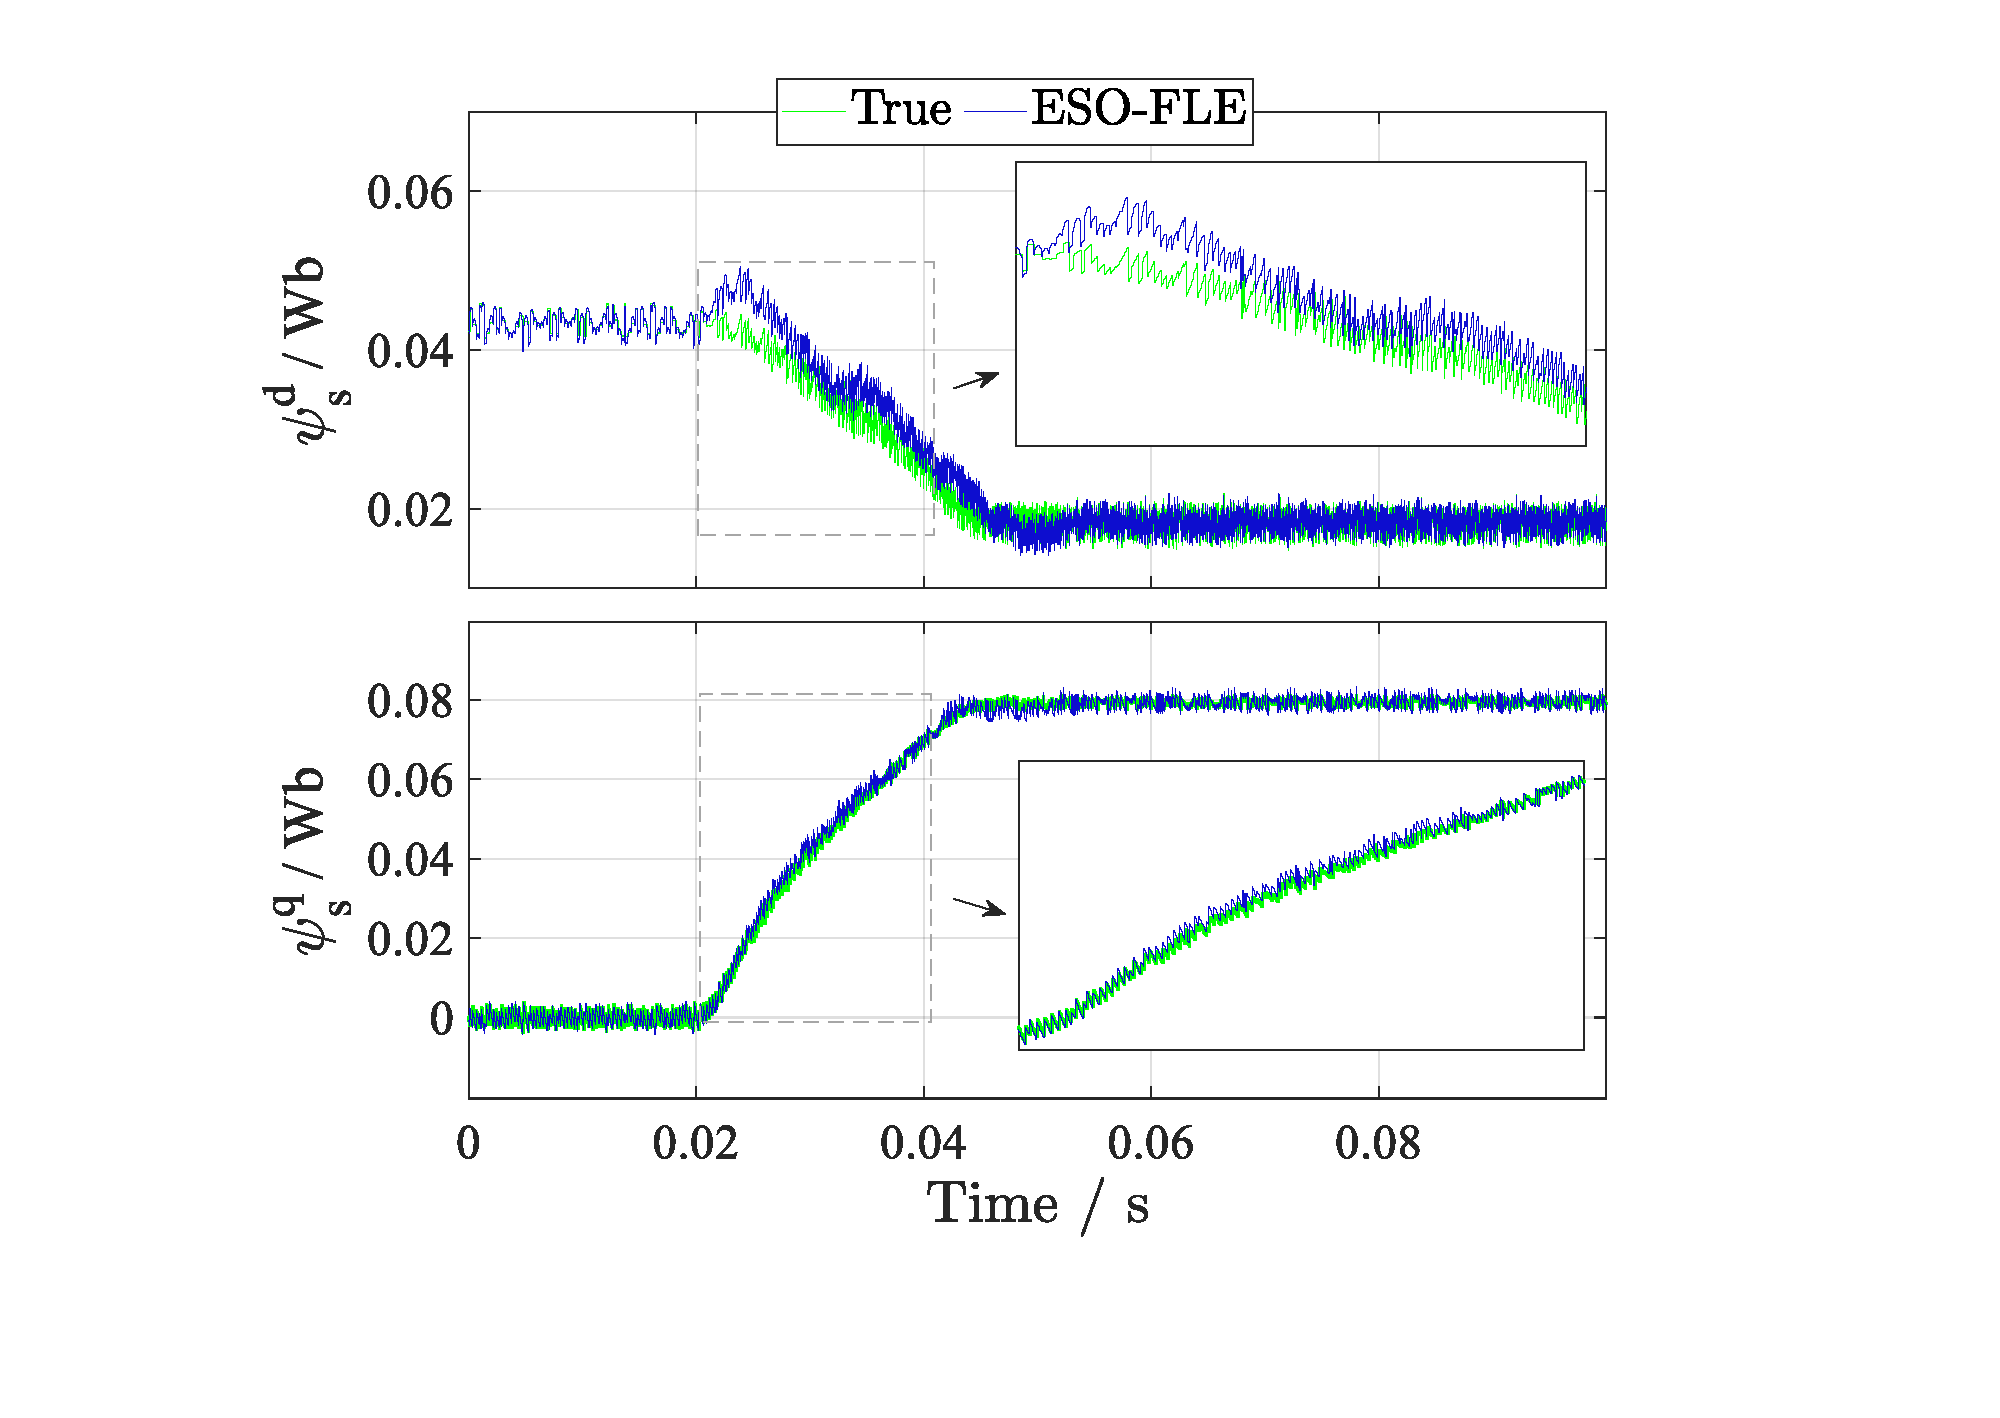
\includegraphics[scale=0.48]{chapters/Fig4.9a.pdf}
        \caption{}
        \label{Fig:4.9a}
    \end{subfigure}
    \vfill
    \begin{subfigure}[c]{1.0\columnwidth}
        \centering
        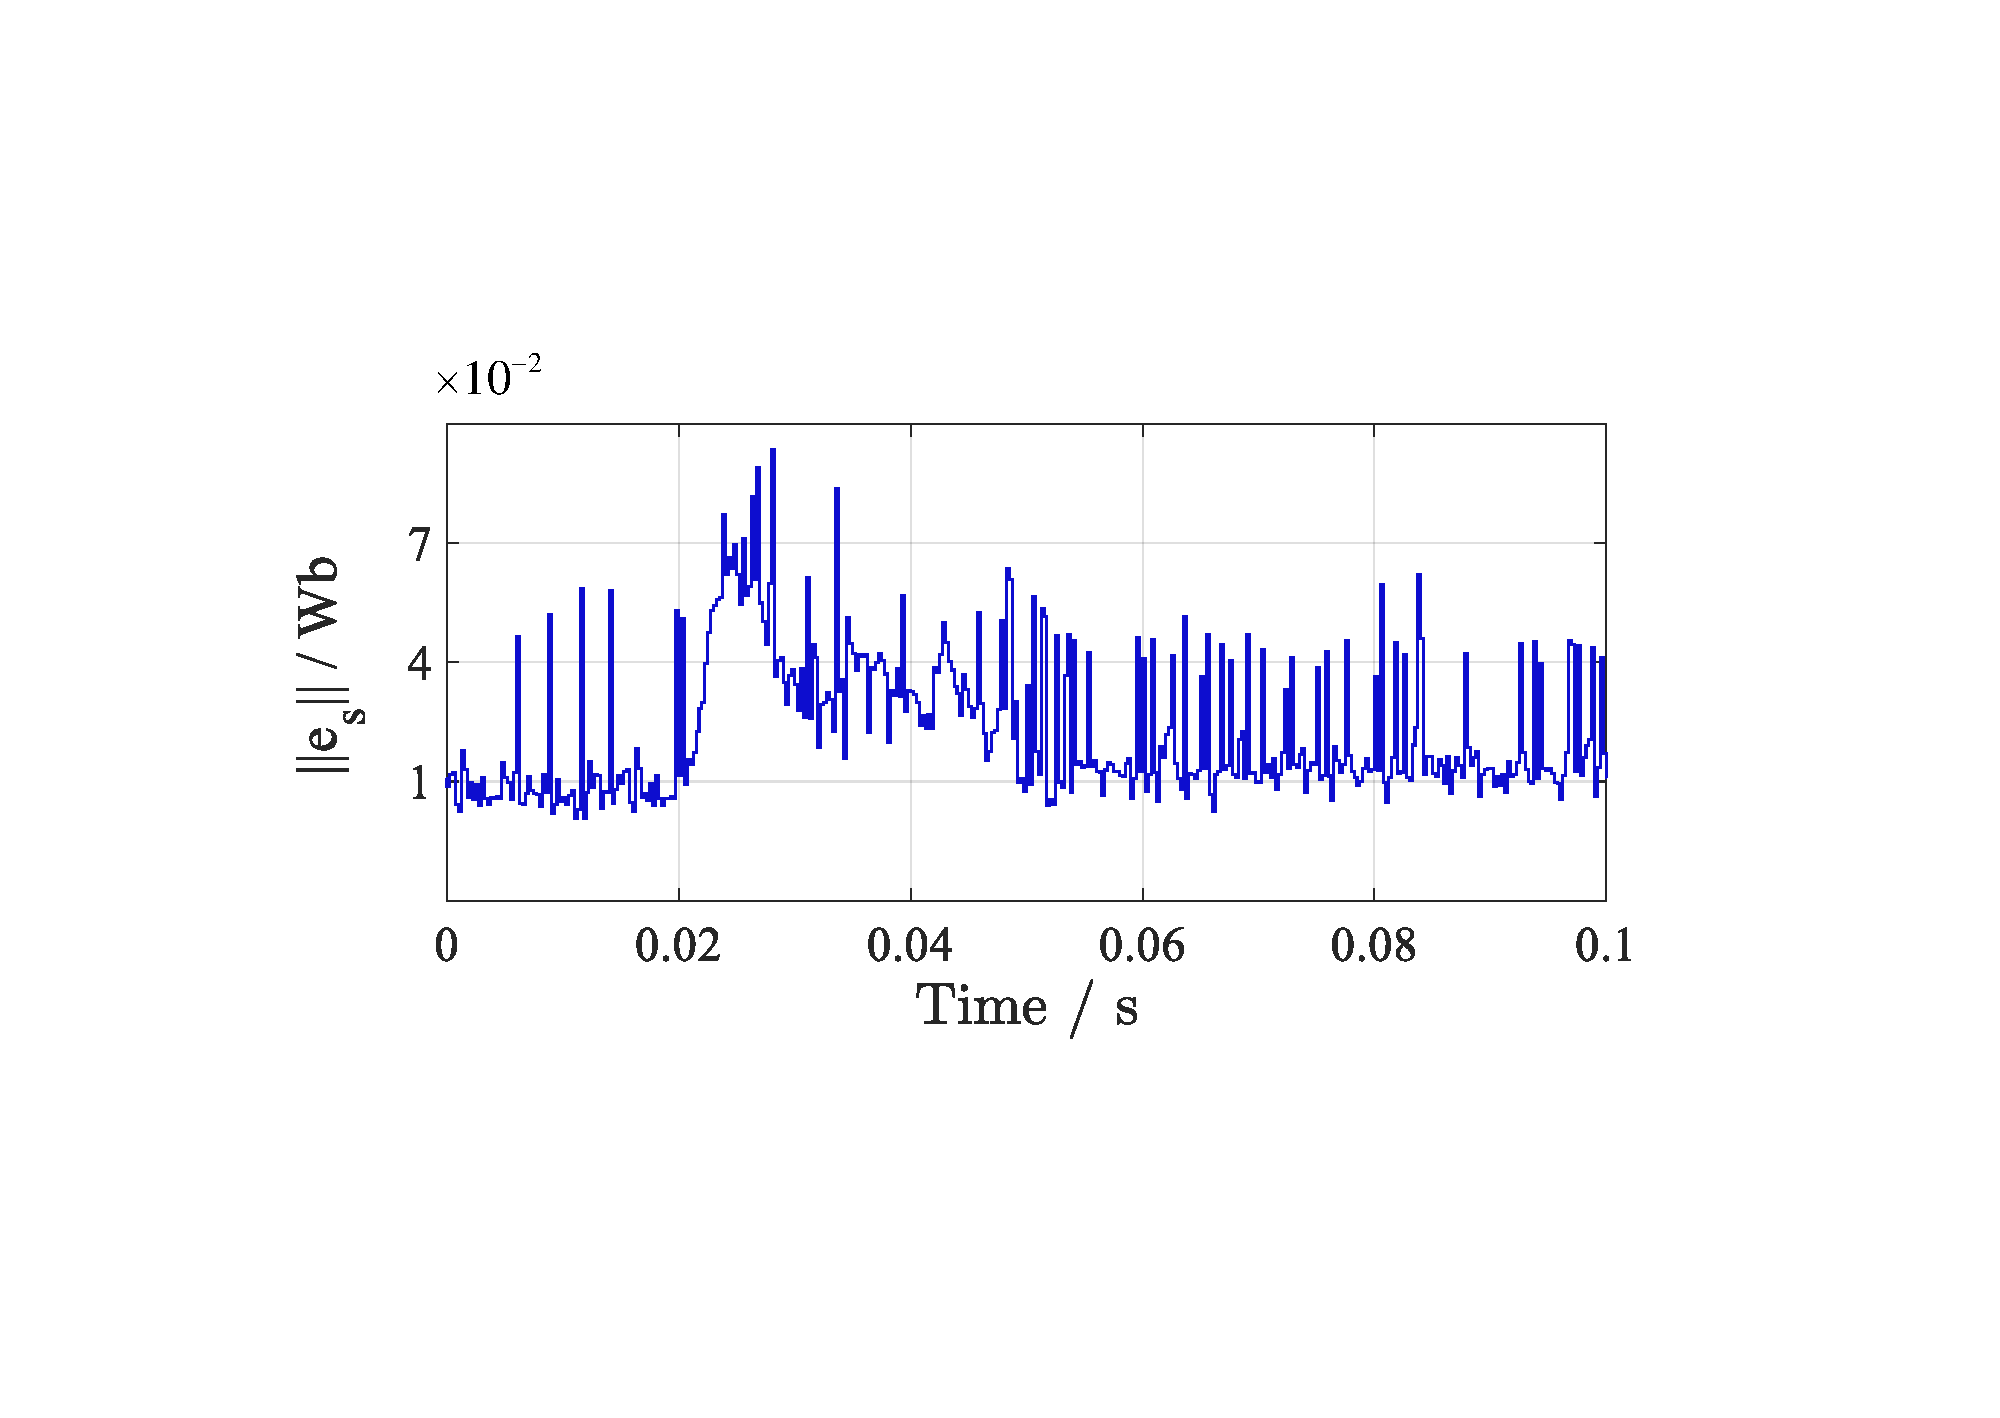
\includegraphics[scale=0.48]{chapters/Fig4.9b.pdf}
        \caption{}
        \label{Fig:4.9b}
    \end{subfigure}
    \caption{Transient estimation performance of the proposed ESO-FLE (a) Flux linkage estimates (b) The corresponding estimation error norm $||\mathbf{e}_s||$.}
    \label{Fig:4.9}
\end{figure}However, as shown in the simulation results of Fig. \ref{Fig:4.9a} and Fig. \ref{Fig:4.9b}, the improved transient estimation performance despite parameter inaccuracies indicates that assuming nonlinear flux linkage $\Delta\mathbf{\psi}^{dq}_s$ as ramp disturbance signals with a constant slope is reasonable.

\section{Validation of the Proposed IE-PU-FLE}
Likewise, the ESO-FLE, the simulation scenarios for verifying the estimation performance of the proposed IE-PU-FLE are as follows: (i) The estimation performance was verified using $q$-axis nominal inductance ($L^q_{s,0}$) under two conditions with a constant mechanical speed of 500 RPM while the torque increased from 0 to 180 Nm, and with the mechanical speed varying from 200 RPM to 1800 RPM while the torque changed from -180 Nm to 180 Nm (In Figs. \ref{Fig:4.4}, \ref{Fig:4.5} and \ref{Fig:4.6}). (ii) The transient estimation performance was examined by updating the inaccurate initial nominal inductance ($\hat L^q_{s,0}:=2L^{q}_{s,0}$) to the actual inductance while the mechanical speed increased from 200 RPM to 1200 RPM and the torque frequently changed from -180 Nm to 180 Nm (In Figs. \ref{Fig:4.7} and \ref{Fig:4.8}). In all scenarios, a gain matrix selected for a constant mechanical speed of 500 RPM was used for IE-PU-FLE. The observer parameters used to verify the estimation performance of the proposed ESO-FLE are listed in Table \ref{Tab4.3}.

\begin{table}[h]
\caption{Observer parameters for IE-PU-FLE}\label{Tab4.3}
\centering
\begin{tabular}{l c}
\hline
\textbf{Parameter} & \textbf{Value}  \\ \midrule
Feedback gain matrix & $\mathbf{F}(419\frac{\text{rad}}{\text{s}})=\begin{bmatrix}
    1271.25 & 564.01\\
    -545.63 & 1271.10\\
    0.012 & -977.27\\
    964.47 & 8.82
\end{bmatrix}$\\
\\
Nominal inductance & $L^{q}_{s,0}=0.28$mH\\
\\
\textit{Guessed} nominal inductance & $\hat{L} ^{q}_{s,0}= 2\times0.28$mH
\\
\\
Forgetting factor & $\beta = 600$
\\
\\
\hline
\end{tabular}
\end{table}
\newpage
\begin{figure}[h]
    \centering
    \begin{subfigure}[b]{0.80\textwidth}
        \centering
        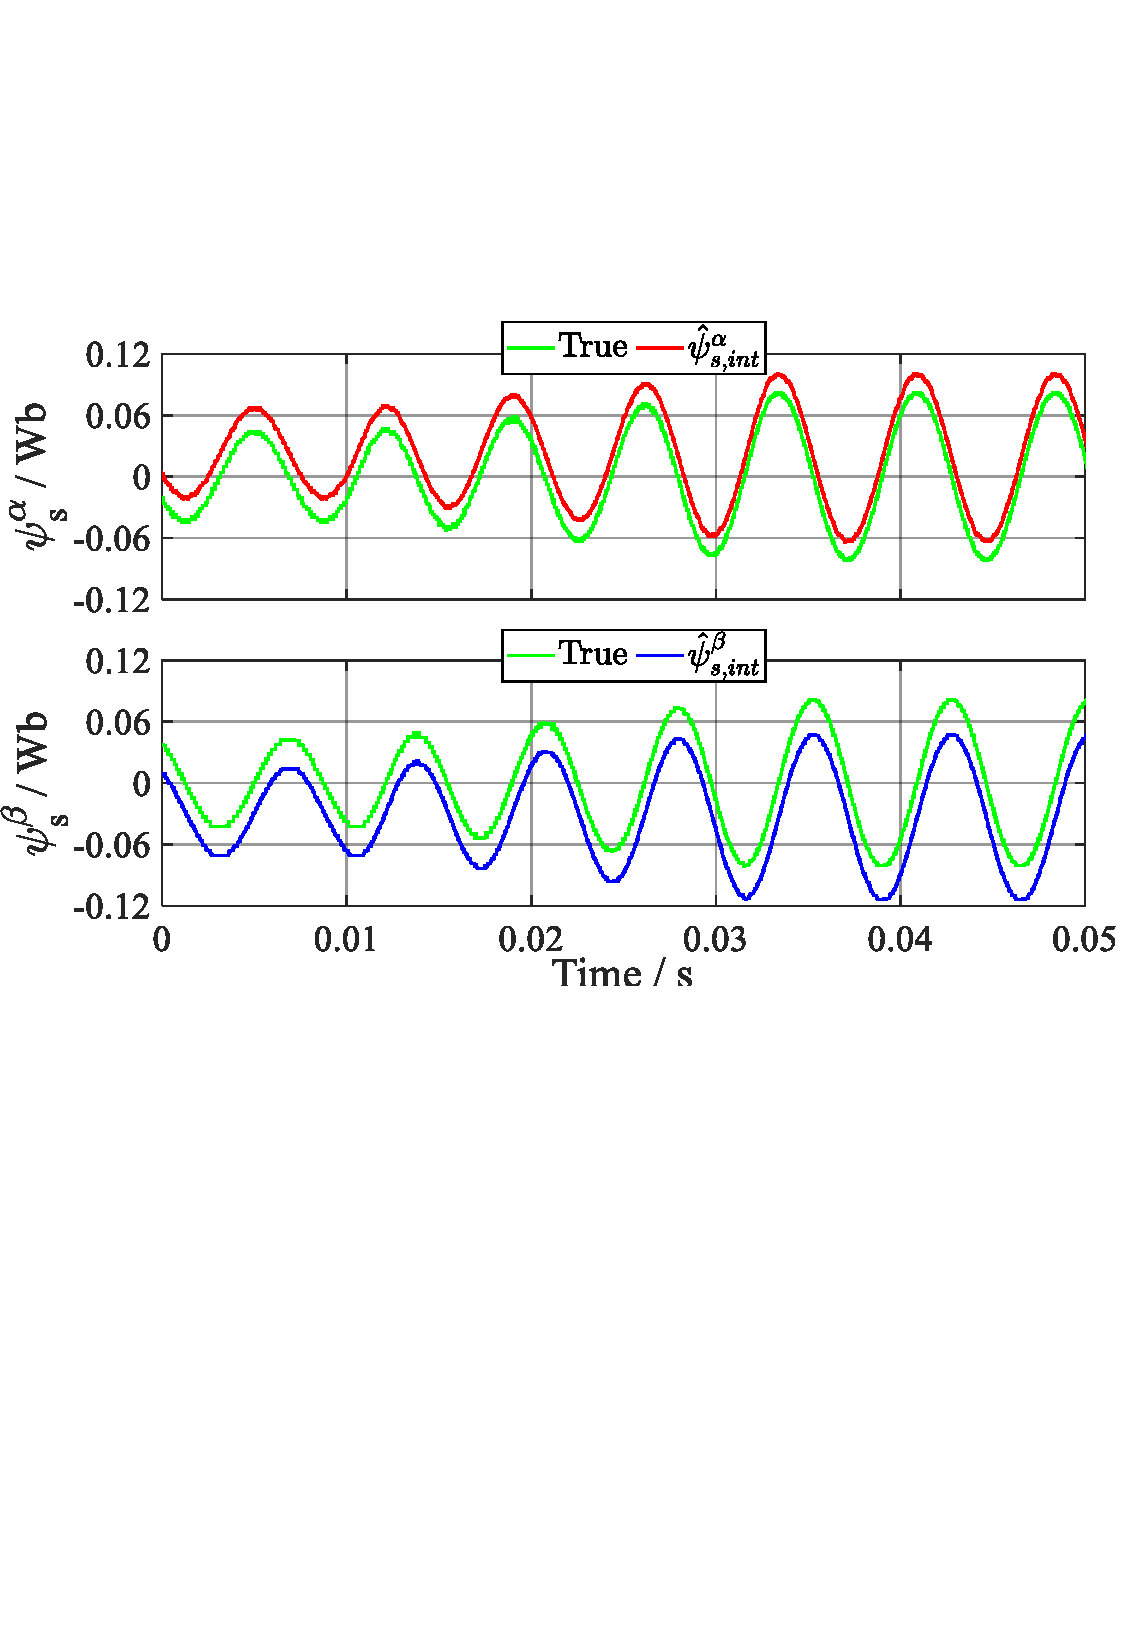
\includegraphics[scale=0.57]{chapters/Fig4.4a.pdf}
        \caption{}
        \label{Fig:4.4a}
    \end{subfigure}
    \vfill
    \begin{subfigure}[b]{0.80\textwidth}
        \centering
        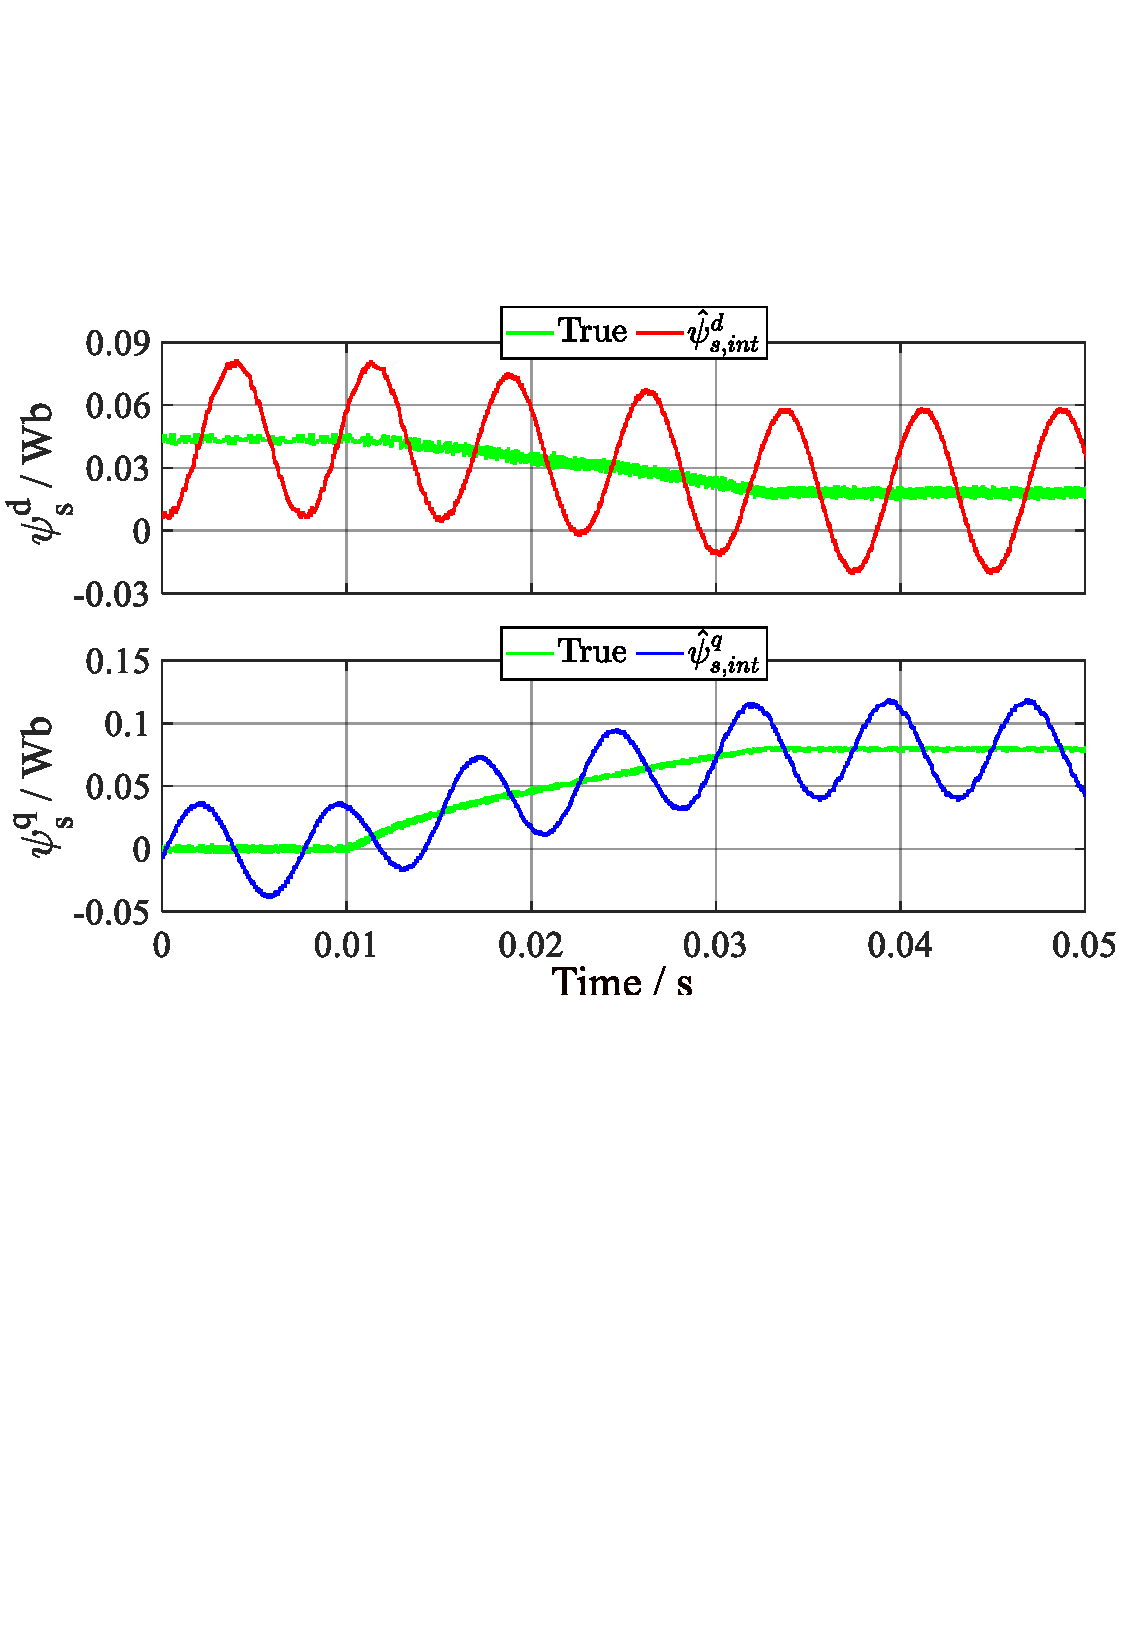
\includegraphics[scale=0.57]{chapters/Fig4.4b.pdf}
        \caption{}
        \label{Fig:4.4b}
    \end{subfigure}
    \caption{Stator flux linkage estimates (a) in the $(\alpha,\beta)$-reference frame and (b) in the $(d,q)$-reference frame without using the integration error estimator.}
    \label{Fig:4.4}
\end{figure}

Figures \ref{Fig:4.4} and \ref{Fig:4.5} show the estimation results without and with the integration error estimator, respectively. Figure \ref{Fig:4.4a} demonstrates that the flux estimates had offsets $\mathbf{O}^{\alpha\beta}_s$ in the ($\alpha$,$\beta$)-reference frame due to inaccurate integration because the integration error was not estimated and compensated. \begin{figure}[H]
    \centering
    \begin{subfigure}[b]{0.80\textwidth}
        \centering
        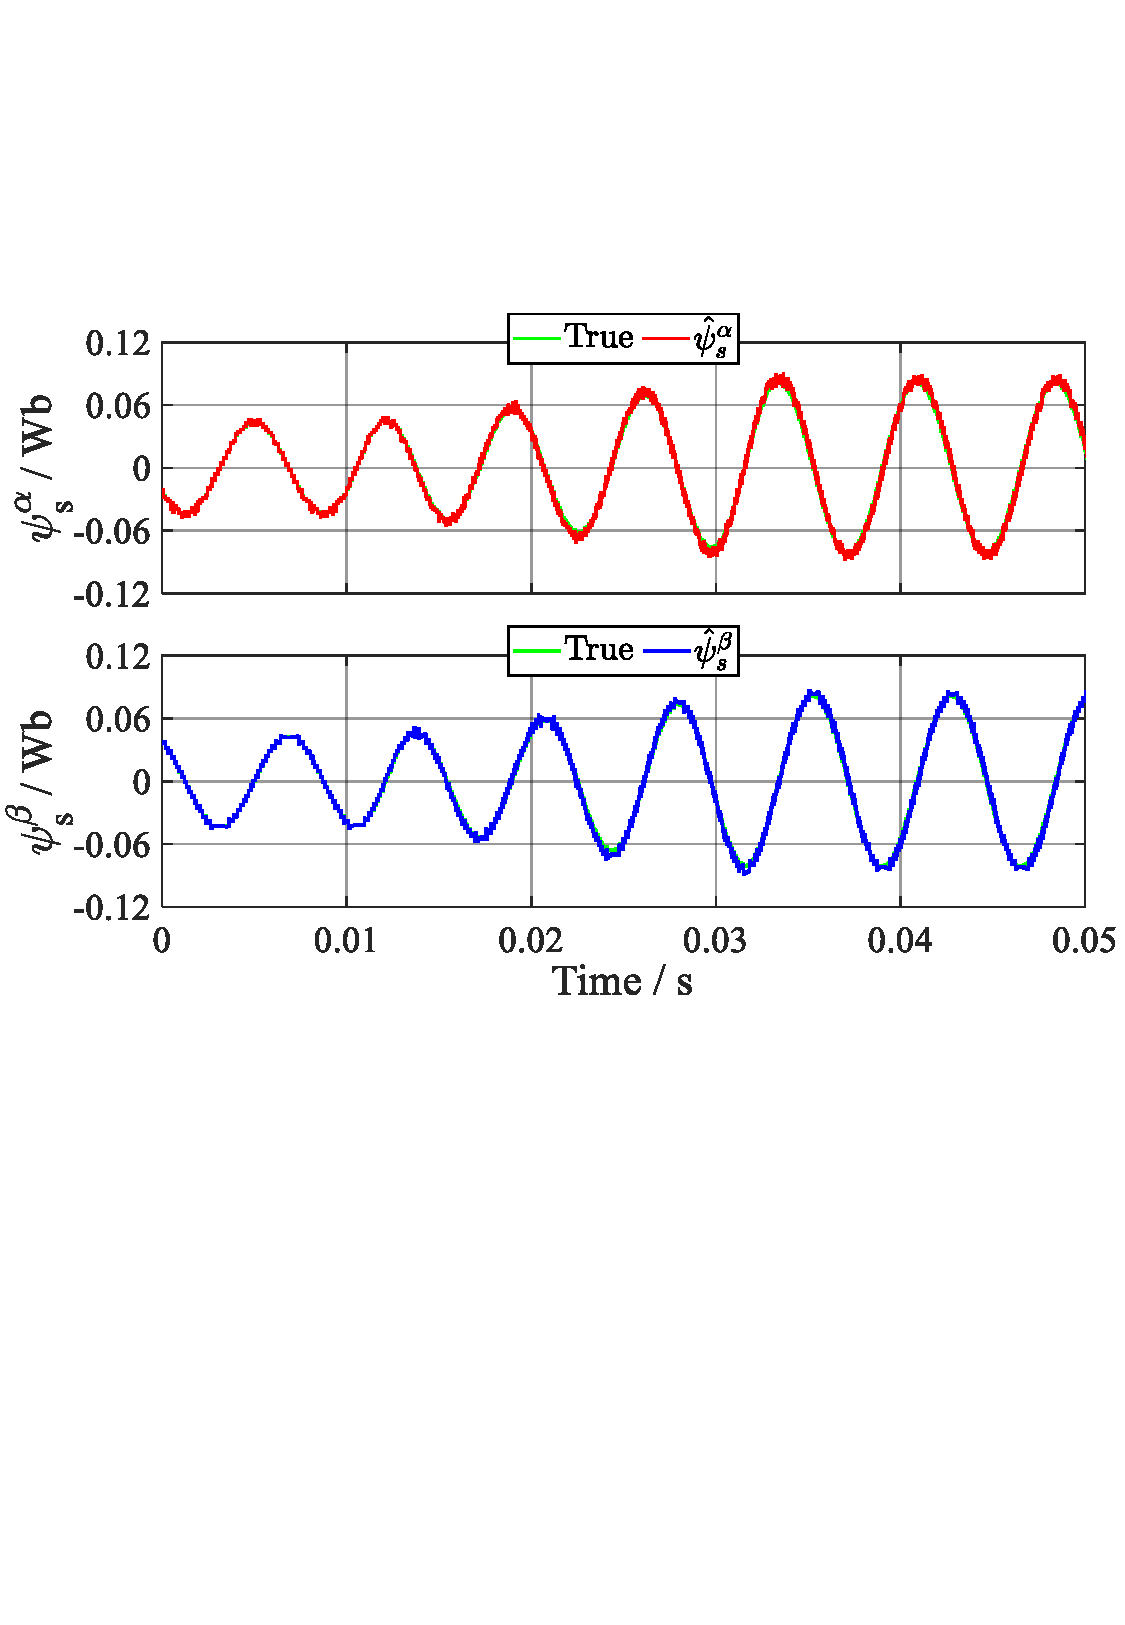
\includegraphics[scale=0.55]{chapters/Fig4.5a.pdf}
        \caption{}
        \label{Fig:4.5a}
    \end{subfigure}
    \vfill
    \begin{subfigure}[b]{0.80\textwidth}
        \centering
        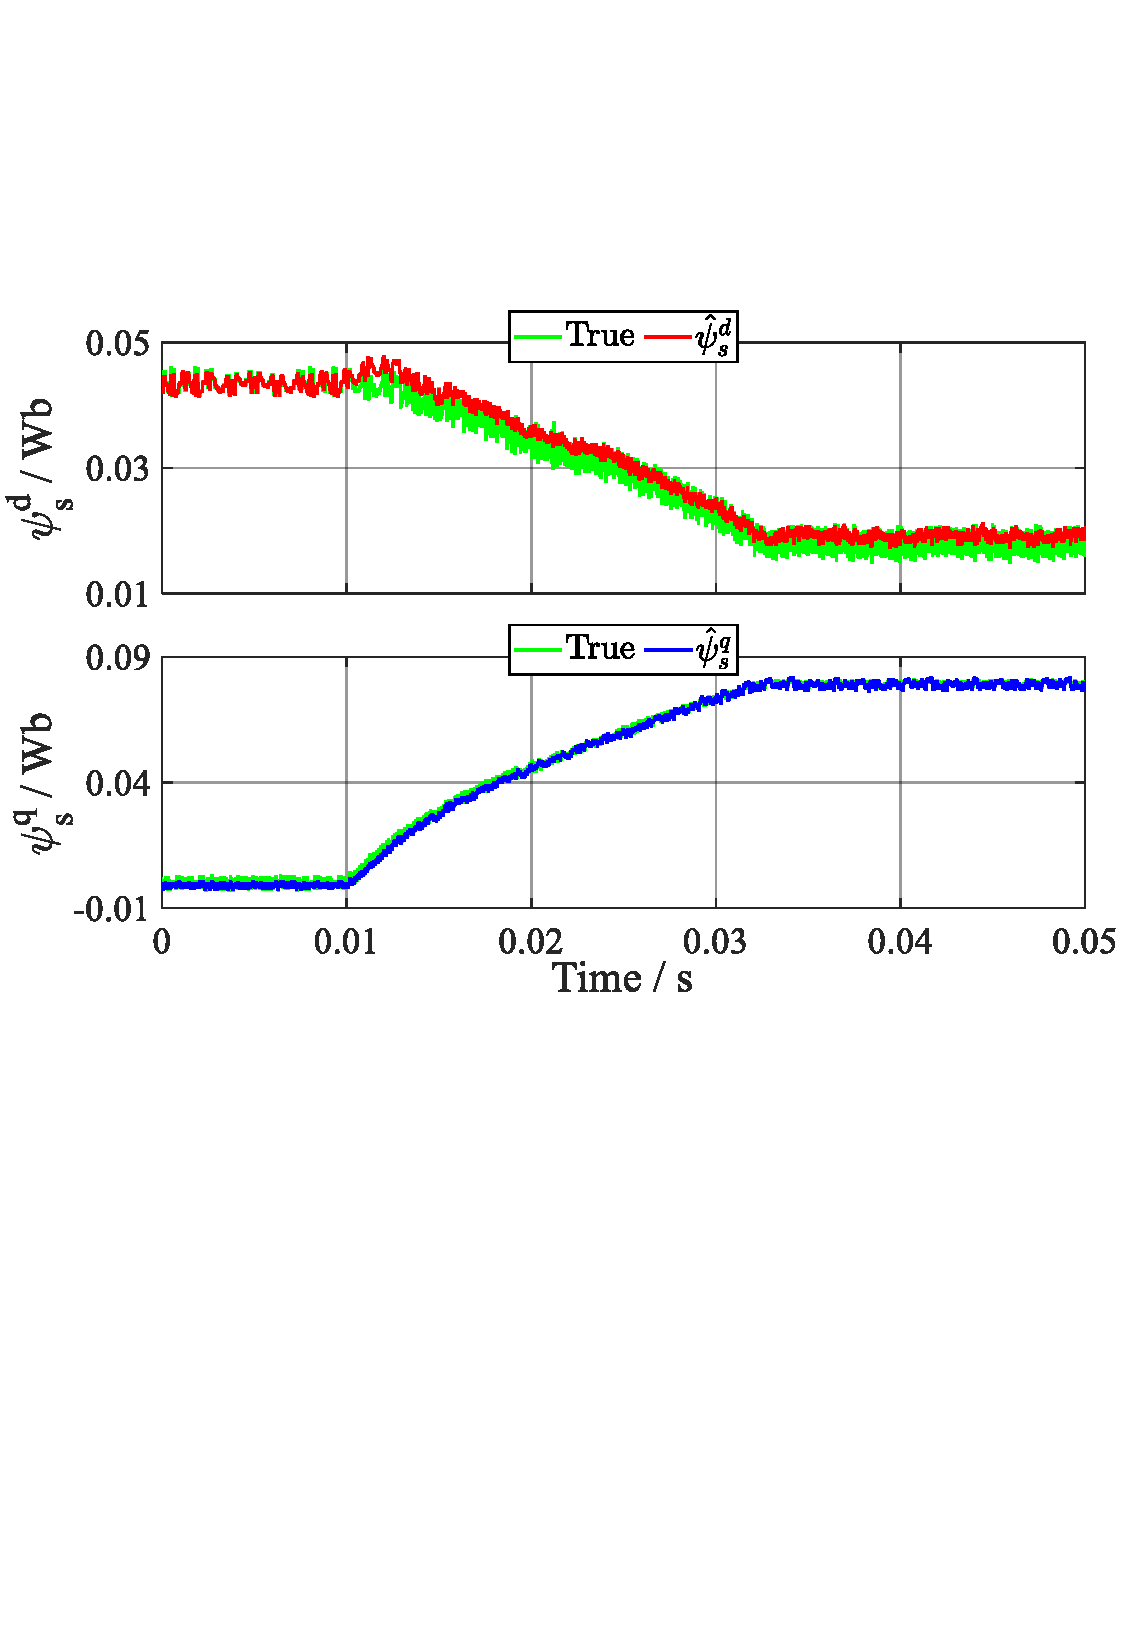
\includegraphics[scale=0.55]{chapters/Fig4.5b.pdf}
        \caption{}
        \label{Fig:4.5b}
    \end{subfigure}
        \vfill
    \begin{subfigure}[b]{0.80\textwidth}
        \centering
        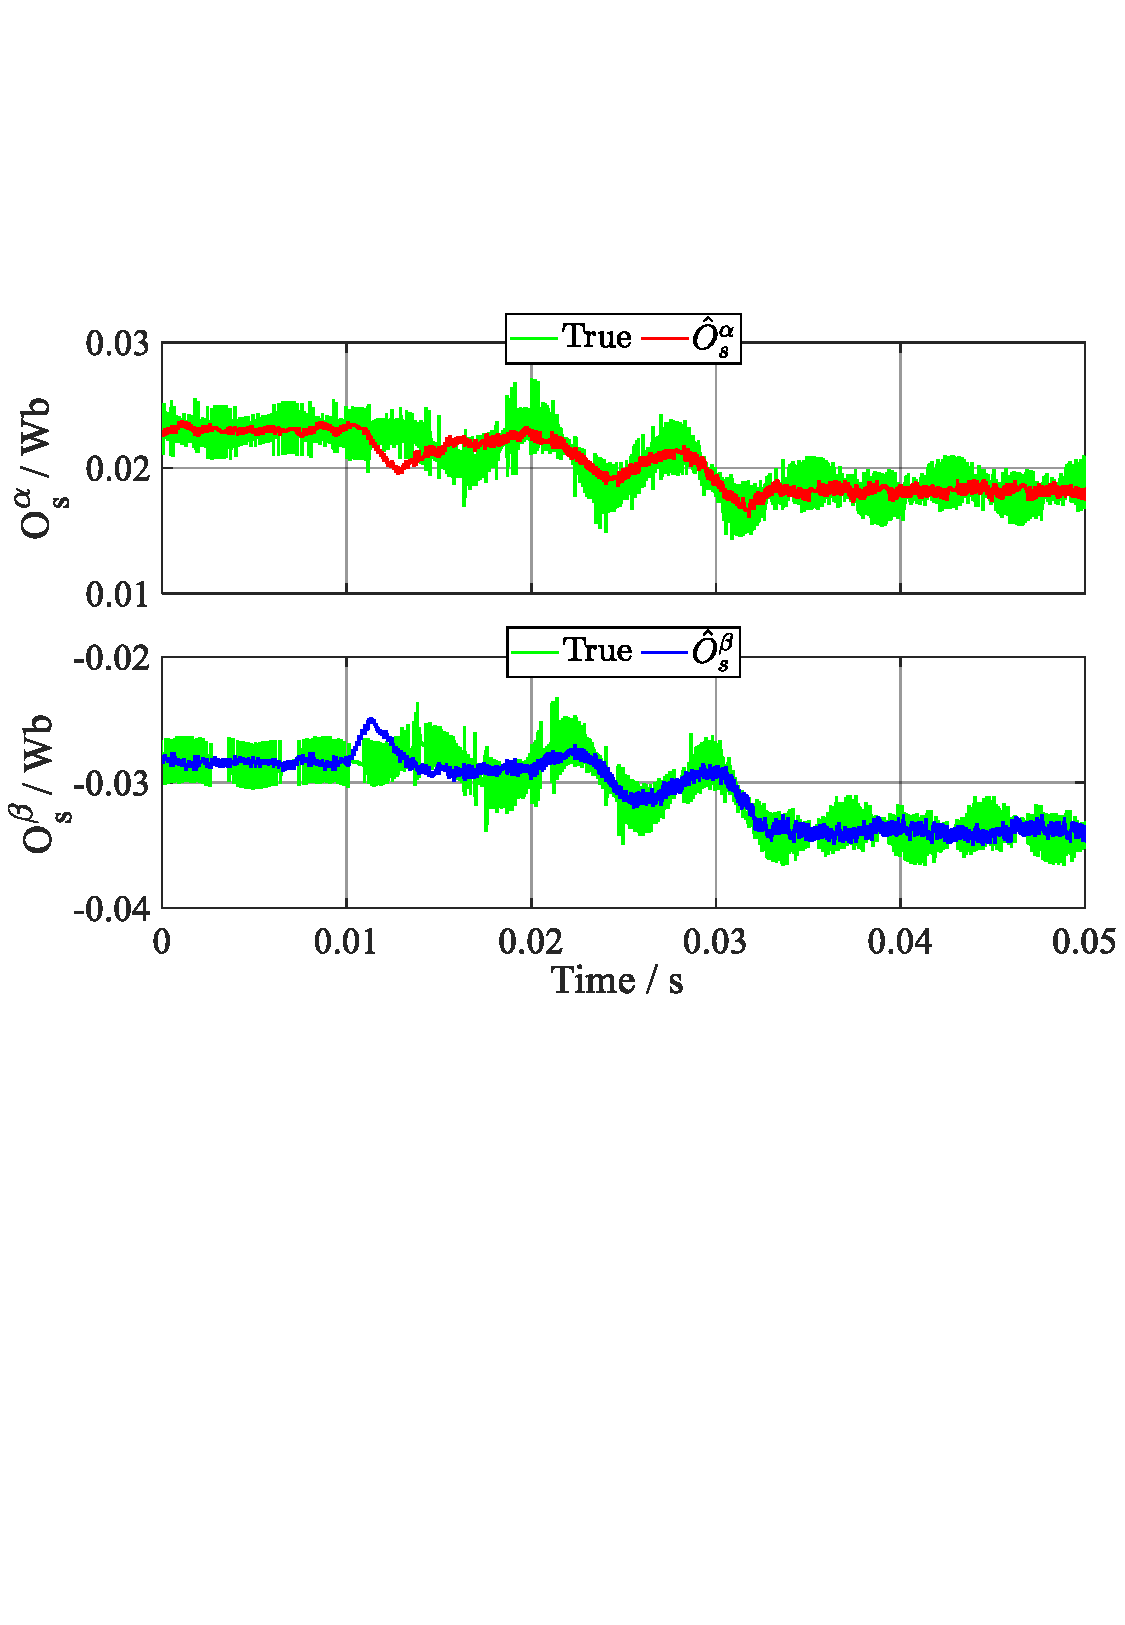
\includegraphics[scale=0.55]{chapters/Fig4.5c.pdf}
        \caption{}
        \label{Fig:4.5c}
    \end{subfigure}
    \caption{Stator flux linkage estimates (a) in the $(\alpha,\beta)$-reference frame and (b) in the $(d,q)$-reference frame using the integration error estimator. (c) The corresponding integration estimates}
    \label{Fig:4.5}
\end{figure}Figure \ref{Fig:4.4b} shows that these offsets in the ($\alpha$,$\beta$)-reference frame were transformed into oscillating components in the rotating ($d$,$q$)-reference frame, which deteriorated the estimation performance. In contrast, Figure \ref{Fig:4.5a} shows that using the integration error estimator, the integration error was compensated, allowing the estimates in the ($\alpha$,$\beta$)-reference frame to accurately track the true values. Consequently, as shown in Fig. \ref{Fig:4.5b}, the estimates in the ($d$,$q$)-reference frame also accurately tracked the true values. This accurate estimation was possible because the integration error was estimated online and compensated in the integration result, as shown in Fig. \ref{Fig:4.5c}.

Figure \ref{Fig:4.6} shows the flux linkage estimates and integration error estimates ($\hat{\boldsymbol{\psi}}^{dq}_s$ and $\hat{\mathbf{O}}^{\alpha\beta}_s$) under different operating conditions for the proposed IE-PU-FLE. At $t=0.05$ seconds, when the mechanical speed was 200 RPM and the torque increased from 0 to 180 Nm, there was an overshoot in the flux estimates due to the observer gain matrix being designed for a fixed speed of 500 RPM, causing estimation errors. However, excluding the low-speed region (after t = 0.07), even under varying torque conditions, the proposed IE-PU-FLE accurately estimated and compensated for the integration error with the fixed observer gain, demonstrating excellent estimation performance in both transient and steady states. Therefore, it is demonstrated that the proposed IE-PU-FLE significantly improves the transient and steady-state performance with the nominal inductance parameter over a wide range of speeds.

\begin{figure}[H]
    \centering
    \includegraphics[scale=0.50]{chapters/Fig4.6.pdf}
    \caption{Stator flux linkage and integration error estimates in the ($d$,$q$)-reference frame}
    \label{Fig:4.6}
\end{figure}
\newpage
\begin{figure}[H]
    \centering
    \includegraphics[scale=0.65]{chapters/Fig4.7.pdf}
    \caption{Proposed stator flux linkage estimator based on the integration error estimator}
    \label{Fig:4.7}
\end{figure}

Figure \ref{Fig:4.7} shows the flux estimates ($\hat{\boldsymbol{\psi}}^{dq}_s$) and $q$-axis inductance estimates ($\hat{L}^{q}_s$) for the proposed IE-PU-FLE under different operating conditions when the nominal inductance parameters are inaccurate. Where the mechanical speed increased linearly from 200 RPM to 1200 RPM, the initial $q$-axis inductance was twice the actual value from $t=0$ to $t=0.02$. However, from $t=0.02$, as the torque (current) decreased to -180 Nm, the inductance estimate became closer to the actual value, thereby reducing the estimation error of the flux estimate in transient state. Additionally, when the torque changed periodically, the $q$-axis inductance was updated online, improving transient estimation performance. Therefore, the proposed IE-PU-FLE method, based on an adaptive observer, was verified through extensive simulation scenarios to be robust against parameter variations by updating the observer's $q$-axis inductance to the actual value online across a wide range of operating conditions, thereby enhancing both transient and steady-state estimation performance.

\section{Performance Comparison between DOB-FLE and the Proposed Estimators}

To compare the flux estimation performance of the proposed ESO-FLE and IE-PU-FLE with the existing DOB-FLE, the gain matrix ${{\boldsymbol{F}({\omega}_{r})}}$ was designed to have a bandwidth of approximately 100 Hz for the observer feedback matrix ${{\boldsymbol{A}}({\omega}_{r})} - {{\boldsymbol{F}({\omega}_{r})}} {{\boldsymbol{C}}}$ at a constant mechanical speed of 500 RPM. In this setup, the nominal inductance parameters of the observers were inaccurately set to half of the actual values for each case to compare the transient estimation performance.

Figure \ref{Fig:4.8} shows the stator flux linkage estimates and estimation error norms of IE-PU-FLE, ESO-FLE, and DOB-FLE in the ($d$,$q$)-reference frame, as well as the $q$-axis inductance estimate of IE-PU-FLE, as the torque changes from  -180 Nm to 180 Nm and mechanical speed varies from 200 RPM to 1000 RPM. 

The estimates of DOB-FLE did not exhibit estimation errors in steady state, but in transient state (especially under low-speed conditions between 0.05 seconds and 0.07 seconds), flux estimation errors occurred and did not converge to the true values. Because DOB-FLE assumes the nonlinear flux $\Delta\boldsymbol{\psi}^{dq}_s$ as step signals, it can only satisfy estimation performance in steady state. However, in the transient state, it fails to account for additional disturbances caused by parameter inaccuracies, resulting in significant estimation errors in the flux estimates. \begin{figure}[!t]
    \centering
    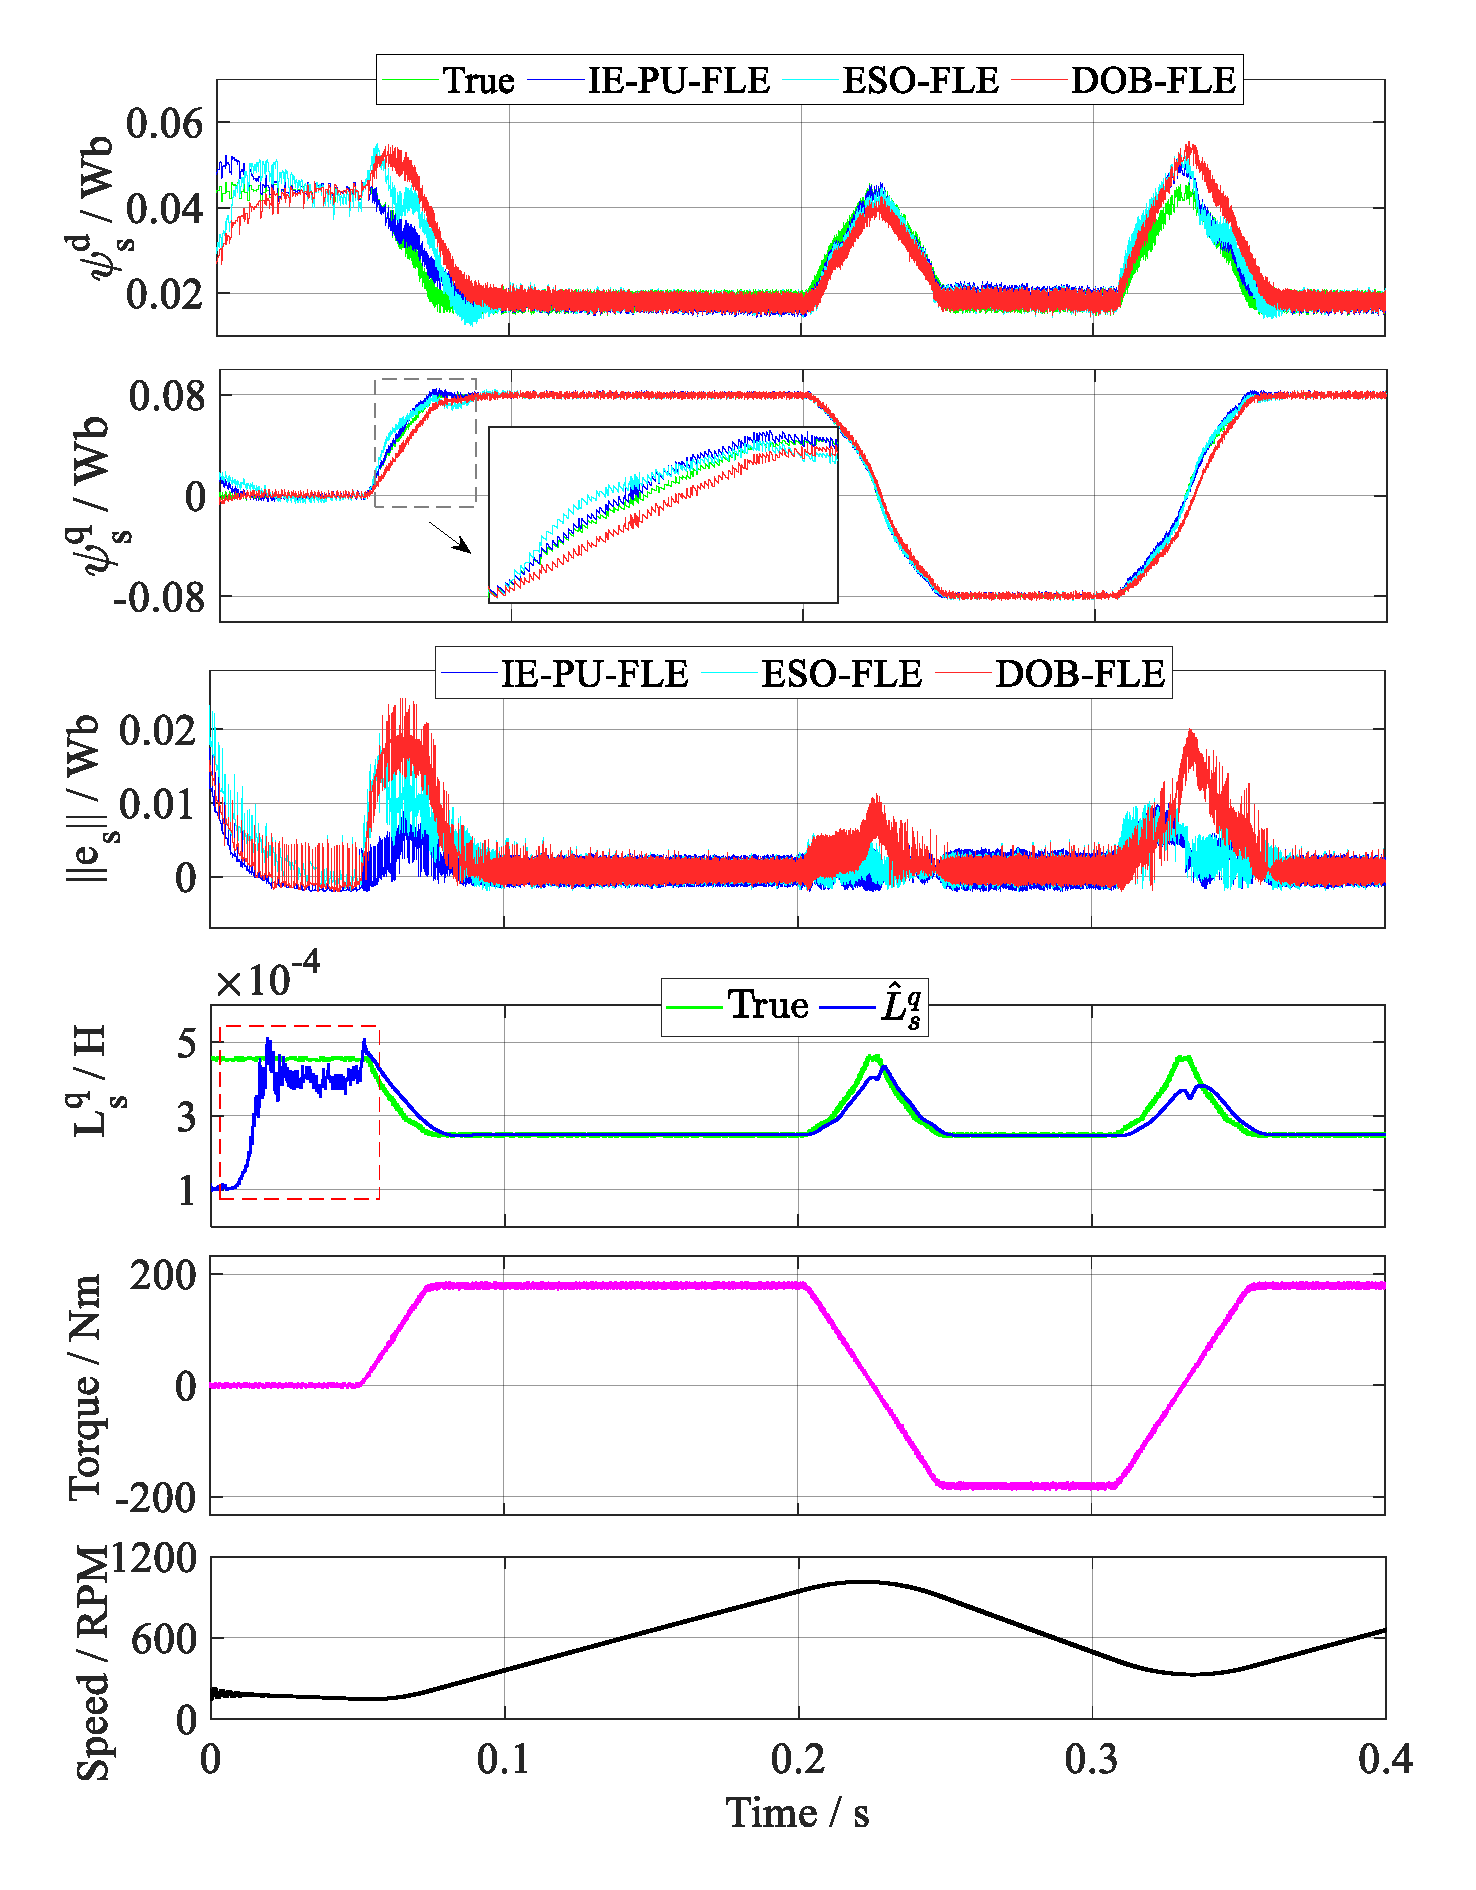
\includegraphics[scale=0.58]{chapters/Fig4.8.pdf}
    \caption{Estimation performance comparison of the proposed ESO-FLE, IE-PU-FLE, and DOB-FLE. }
    \label{Fig:4.8}
\end{figure} 

By contrast, as seen in Fig.\ref{Fig:4.8}, ESO-FLE demonstrated improved transient performance compared to DOB-FLE. This enhancement is attributed to ESO-FLE's approach of treating the nonlinear flux term $\Delta\boldsymbol{\psi}^{dq}_s$ as time-varying ramp disturbance signals, unlike DOB-FLE, which assumes these disturbances to be constants. It is also evident that only the estimation error of ESO-FLE decreased compared to DOB-FLE during transient states.

Furthermore, IE-PU-FLE demonstrated significant improvements in both transient and steady-state estimation performance by using RLS to update the $q$-axis inductance parameter in real-time and employing an adaptive observer to continuously compensate for parameter errors, thereby improving the estimation performance, even when the initial inductance parameters were inaccurately set. However, as shown in the $q$-axis inductance estimates between $t=0.02$ and $0.05$, if the input signal does not satisfy the PE condition or if the input signals are insufficient (i.e. $d$-$q$ axis currents are small), estimation errors in the inductance estimates may occur.






\end{spacing}

%---------
% Chapter 5 Conclusion
%%%%%%%%%%%%%%%%%%%%%%%%%%%%%%%%%%%%

\begin{spacing}{2.0}

\chapter{Conclusion and Future Work}\label{chapter5}
\subsubsection{Conclusion}
In this thesis, two flux linkage estimators (ESO-FLE and IE-PU-FLE) were presented, which are applicable to any nonlinear synchronous machine.  Both estimators are designed as state observers in the time domain, eliminating the need for applying filters for estimation, thus avoiding any magnitude and phase distortions in the estimates. Additionally, ESO-FLE assumes nonlinear flux as ramp disturbance signals, while IE-PU-FLE uses RLS to estimate parameter variations online and compensates for parameter estimation errors with an adaptive observer, enabling both observers to handle parameter inaccuracies and improve transient estimation performance. Simulation results obtained using a 35-kW PMSM drive demonstrated that the proposed estimator closely tracked the true trajectories of the stator flux linkages under various operating conditions with better transient performance than the conventional estimators. 

\subsubsection{Future Work}

Future research will (i) focus on the optimal observer gain design to ensure stability and convergence considering parameter and speed variations (e.g., gain design based on LMI (Linear Matrix Inequality)), (ii) estimate flux linkage considering inverter nonlinearity (e.g., estimated based on Neural Network) or core losses, (iii) extract static or dynamic inductance based on online flux estimates (e.g., conducting optimal current control or MTPA algorithm), and finally, validate the performance and robustness of the proposed approach in the laboratory through experimental results.

\end{spacing}

%---------

% summary
%---------

%-----------------------------------------------------------------------
% This is the end of the main thesis body.

%-----------------------------------------------------------------------
% Input the list of references.
\bibliographystyle{ieeetr}
\bibliography{biblist}


%%%%%%%%%%%%%%%%%%%%%%%%%%%%%%%%%%%%%%%%%%%%%%%%
% Appendix
% You can comment out if you do not need appendix
%%%%%%%%%%%%%%%%%%%%%%%%%%%%%%%%%%%%%%%%%%%%%%%%
\begin{spacing}{2.0}

%%%%%%%%%%%%%%%%%%%%%%%%%%%%%%%%%%%%%%%%%%%%%%%%
% Appendix
%%%%%%%%%%%%%%%%%%%%%%%%%%%%%%%%%%%%%%%%%%%%%%%%

%\appendixpage
\appendix
\chapter{Recursive Least Square}\label{Appen1}
The unknown parameters appear in a linear form, such as in the linear parametric model
\begin{equation}
    \mathbf{z} = {\theta^*}^\top \mathbf{u}
\end{equation}
where \(z\) is the output signal, \({\theta^*}^\top\) denotes the unknown parameter to be estimated, and \(\mathbf{u}\) represents the input signals. The estimate of $\mathbf{z}$ is expressed as
\begin{equation}
\hat{\mathbf{z}} = \theta\mathbf{u},
\end{equation}
where \(\hat{\mathbf{z}}\) and \(\theta\) denote the estimate of \(\mathbf{z}\) and the estimated parameter of \(\theta^*\), respectively and the parameter estimation error is defined as
\begin{equation}
\boldsymbol{\epsilon} =\mathbf{z} - \hat{\mathbf{z}} = \mathbf{z} - \theta^\top \boldsymbol{u}.
\end{equation}
To estimate the parameter $\theta^*$, the integral cost function \cite{c3.2_4} is considered as follows:
\begin{equation}
J(\theta) = \frac{1}{2} \int_{0}^{t} e^{-\beta(t-\tau)} \left[ \mathbf{z}(\tau) - \theta(t) \boldsymbol{u}(\tau) \right]^2 d\tau + \frac{1}{2} e^{-\beta t} (\theta - \theta_0)^\top Q_0 (\theta - \theta_0),
\end{equation}
where \( Q_0 > 0 \), \( \beta > 0 \), and \( \theta_0 = \theta(0) \), which include discounting of past data and a penalty on the initial estimate \(\theta_0\) of \(\theta^*\). Since \( J(\theta) \) is a convex function of \(\theta\) at each time \( t \), the global minimum can be achieved when the gradient of the cost function is zero, which gives \(\theta(t)\) as follows:
\begin{equation}
\theta(t) = \Gamma(t) \left[ e^{-\beta t} Q_0 \theta_0 + \int_{0}^{t} e^{-\beta (t - \tau)} \mathbf{z}(\tau) \boldsymbol{u}(\tau) d\tau \right],
\end{equation}
where
\begin{equation}
\Gamma(t) = \left[ e^{-\beta t} Q_0 + \int_{0}^{t} e^{-\beta(t - \tau)} \mathbf{u}(\tau)^\top \mathbf{u}(\tau) d\tau \right]^{-1},
\end{equation}
with \( Q_0 > 0 \) and \( \mathbf{u}^\top \mathbf{u} \) being positive semidefinite, \( \Gamma(t) \) exists at each time \( t \). By Using the identity, the differential equation of $\Gamma(t)$ can be expressed as
\begin{equation}
\begin{aligned}
\frac{d}{dt} \left( \Gamma \Gamma^{-1} \right) = \dot{\Gamma} \Gamma^{-1} + \Gamma \frac{d}{dt} \left( \Gamma^{-1} \right) = 0,\\
    \dot{\Gamma} = \beta \Gamma - \Gamma \boldsymbol{u}^\top \boldsymbol{u} \Gamma, \quad \Gamma(0) = \Gamma_0 = Q_0^{-1},
\end{aligned}
\end{equation}
Finally, differentiating the equation (\ref{eqn:3.23}) with respect to \( t \) and using (\ref{eqn:3.21}) and (\ref{eqn:3.25}), the continuous-time recursive least-squares parameter update algorithm with forgetting factor can be expressed as
\begin{equation}
\dot{\theta} = \Gamma \boldsymbol{\epsilon}^\top \boldsymbol{u}. 
\end{equation}
where \(\Gamma\) denotes the covariance matrix and \(\beta\) is called the forgetting factor. Therefore, if the input signal \(\mathbf{u}\) satisfies the PE (Persistent Excitation) condition and \(\theta\) and \(\dot{\theta}\) are uniformly bounded, then \(\theta(t)\) will eventually converge exponentially to the actual parameter \(\theta^*\).
\end{spacing}

%-----------------------------------------------------------------------
% Acknowledgements
% Insert the text between \begin{acknowledgements} and \end{acknowledgements}.
% You can either write the abstract directly here or import a file using the \input command.

%%%%%%%%%%%%%%%%%%%%%%%%%%%%%%%%%%%%%%%%%%
% Acknowledgements by Korean
%%%%%%%%%%%%%%%%%%%%%%%%%%%%%%%%%%%%%%%%%%
\begin{acknowledgements}
\begin{spacing}{2.0}
%%%%%%%%%%%%%%%%%%%%%%%%%%%%%%%%%%%%%%
% Acknowledgements of the thesis in English
%%%%%%%%%%%%%%%%%%%%%%%%%%%%%%%%%%%%%%
\end{spacing}
\end{acknowledgements}


%-----------------------------------------------------------------------
% Input the curriculum vitae.
% You may add as many lines as you need using the syntax of the \item command shown below.
%-----------------------------------------------------------------------



%\input Vitae2.0.tex
%\input thesis-publications.tex

% Insert activity if you have.
%\activity
%Activity Activity Activity Activity Activity Activity Activity Activity
%Activity Activity Activity Activity Activity Activity Activity Activity

% Insert awards if you have.

%-----------------------------------------------------------------------
% This is the end of the thesis.
%
\end{document}
